\documentclass[12pt,oneside,a4paper]{book} % This style for A4 format.

%Packages
\usepackage{ecproject}
\usepackage{graphicx}
\usepackage{tikz}
\usetikzlibrary{calc}
\usepackage[a4paper, margin=1in]{geometry}
\usepackage{float}
\usepackage{qrcode}
%%%Page related
\usepackage{fancyhdr} % for header & footer
\usepackage[hidelinks]{hyperref}
\usepackage[toc, nonumberlist]{glossaries} %For Glossaries - to be loaded only after hyperref package
% For code snippets
\usepackage[listings]{tcolorbox}
    \tcbuselibrary{skins,breakable}
    \tcbuselibrary{theorems}
%\ifIndentPara
\usepackage{indentfirst}
%\fi
\usepackage{setspace}
%%%Table Related
%\usepackage{booktabs}
%\usepackage{makecell}
%\usepackage{multirow}
%\usepackage{multicol}


%% Document settings
\title{Towards Efficient ML Hardware : FPGA Architectural Exploration and PCA Accelerator Design}
\subCode{21EC81P}
\Department[ECE]{Electronics and Communication Engineering}
\academicYear{2024-25}

%%%%%%%%%%%%%%%Minor (or) Major report%%%%%%%%%%%%%%%
%% Uncomment \MinorProject line, if the report is for Minor project.
%\MinorProject

%%%%%%%%%%%%%%%%%%%For PG program%%%%%%%%%%%%%%%%%%%
%% Uncomment \pgProgram command and define appropriate values for \MastersIn{} and \pgProgramName{}

%\pgProgram%
\MastersIn[M.Tech]{Master of Technology}
\pgProgramName{VLSI Design \& Embedded Systems}

%%%%%%%%%%%%%%%%%%%%%%%%%%%%%%%%%%%%%%%%%%%%%%
%% Student Details%%%
\stuNameA{Srivaths Ramasubramanian}
\stuUSNA{1RV21EC168}
%\stuNameB{Nithin M}
%\stuUSNB{1RV16EC006}
%\stuNameC{Subrahmanya K N}
%\stuUSNC{1RV16EC007}
%\stuNameD{Subrahmanya K N}
%\stuUSND{1RV16EC007}

%% Internal Guide%%%%
\guideNameA{Dr. K.S Geetha}
\guideDesignationA{Professor \& Vice Principal}
\guideDeptA{Dept. of ECE}
\guideOrgA{RV College of Engineering}

%%%External Guide%%%%
%\guideNameB{Dr. Ramavenkateshwaran}
%\guideDesignationB{Assistant Professor}
%\guideDeptB{Dept. of ECE}
%\guideOrgB{RV College of Engineering}

%\guideNameC{Dr. Ramavenkateshwaran}
%\guideDesignationC{Assistant Professor}
%\guideDeptC{Dept. of ECE}
%\guideOrgC{RV College of Engineering}

\panelMemberA{Dr. Roopa J}
\panelMemberDesigA{Assistant Professor}
\panelMemberB{Prof. Ravishankar Holla}
\panelMemberDesigB{Assistant Professor}

% Added Ver 3.6
%% Project co-ordonators
\projectMemberA{Dr. Veena Devi S V}
\projectMemberDesigA{Associate Professor}
\projectMemberB{Prof. Sindhu Rajendran}
\projectMemberDesigB{Assistant Professor}


%%%%%%%%%%%%%%%%% Esteemed Members %%%%%%%%%%%%%%%%%%
\HOD{Dr. H V Ravish Aradhya}
\Principal{Dr. K. N. Subramanya}

%%%%%%%%%%%%%%%%%%%%%  QRL %%%%%%%%%%%%%%%%%%%%%%%%%%
\QRurl{}
%\QRurl{https://drive.google.com/open?id=1jm-POmuq-ZZ1tT5m-xAdCDRnwvLZH8q-}

%%%%%%%%%%%%%%%%%%Draft report%%%%%%%%%%%%%%%%%%
\DraftCopy %Not yet implemented, if anyone interested, do contact me at pnarashimaraja@rvce.edu.in (or) narashimaraja@gmail.com
%%%%%%%%%%%%%%%%%%%%%%%%%%%%%%%%%%%%%%%%%%%%%%

%%%%%%%%%%%%%%%%%% Glossaries & Acronyms %%%%%%%%%%%%%%%%%%
\newglossary[sym]{symbolList}{sym1}{sym2}{List of Symbols}
\makeglossaries
% Acronyms
\loadglsentries{./AuxFiles/Glossaries}
\renewcommand{\glspostdescription}{}% To remove dot at the end
%%%%%%%%%%%%%%%%%%%%%%%%%%%%%%%%%%%%%%%%%%%%%%

%%%%%%%%%%%%%%%% Bibliography %%%%%%%%%%%%%%%%%%%%%
\usepackage[backend=bibtex,style=ieee]{biblatex}
% If backend is set to bibtex, then configure texmaker Bi(La)Tex with "bibtex %"
\addbibresource{./AuxFiles/ProjectBib.bib}%Add bib file with extention
%%%%%%%%%%%%%%%%%%%%%%%%%%%%%%%%%%%%%%%%%%%%%%

%%%%%%%%%%%%%%%%WaterMark%%%%%%%%%%%%%%%%%%%%%
%% Use it only after Biblatex
%% Uncomment the following lines for watermarking and run it more than 2 times for proper alignment
\usepackage{background}
\backgroundsetup{scale=1, angle=0, firstpage = false, opacity=1, contents={
\begin{tikzpicture}[remember picture, overlay]
\node at ([yshift=0pt, xshift=0pt]current page.center){
\includegraphics[width=0.6\textwidth]{Figures/RVlogoVecW}};
\end{tikzpicture}
}}
%%%%%%%%%%%%%%%%%%%%%%%%%%%%%%%%%%%%%%%%%%%%%%

\begin{document}
\NoBgThispage% Don't remove this command, even if you want logo on the first page.	
\maketitle
%\pagestyle{empty}
\newpage
\begin{spacing}{1.5}
%%ecproject package is created by P Narashimaraja, Assistant Professor, ECE, RVCE
%Border

\begin{tikzpicture}[remember picture, overlay]
  \draw[line width = 4pt] ($(current page.north west) + (0.75in,-0.75in)$) rectangle ($(current page.south east) + (-0.75in,0.75in)$);
\end{tikzpicture}
\thispagestyle{empty}
\vspace{-1cm}
\begin{center}
\Large\textbf{RV College of Engineering\textsuperscript{\small\textregistered}, Bengaluru} \par
\large{(\textit{Autonomous institution affiliated to VTU, Belagavi})} \par
\large\textbf{Department of \printDepartmentLF}\\
.\hspace{2cm}\\

\includegraphics[width=3cm]{Figures/RV_logoVec}\par
\Large\textbf{\underline{CERTIFICATE}} \par
\end{center}
%\begin{minipage}[b]{\linewidth}
%\large
\begin{spacing}{1.5}
\noindent Certified that the \ifMinor{minor\;}\else{ major\;}\fi project (\printCode)work titled \textbf{\textit{\printTitle}} is carried out by
\ifPG{%
\textbf{\printStuNameA} (\textbf{\printStuUSNA}) who is  bonafide student 
}
\else{
\ifStuNameDUsed{%
\textbf{\printStuNameA } (\textbf{\printStuUSNA}), \textbf{\printStuNameB } (\textbf{\printStuUSNB}), \textbf{\printStuNameC } (\textbf{\printStuUSNC}) and \textbf{\printStuNameD } (\textbf{\printStuUSND})  who are bonafide students 
}\else{% 
\ifStuNameCUsed{%
\textbf{\printStuNameA } (\textbf{\printStuUSNA}), \textbf{\printStuNameB } (\textbf{\printStuUSNB}) and \textbf{\printStuNameC } (\textbf{\printStuUSNC})  who are bonafide students 
}\else{%
\ifStuNameBUsed{%
\textbf{\printStuNameA} (\textbf{\printStuUSNA}) and \textbf{\printStuNameB} (\textbf{\printStuUSNB})  who are bonafide students 
}\else{%
\textbf{\printStuNameA} (\textbf{\printStuUSNA}) who is  bonafide student 
}
\fi
}\fi
}\fi
}\fi
of RV College of Engineering, Bengaluru, in partial fulfillment of the requirements for the degree of  \ifPG \textbf{\printMastersInLF} in \textbf{\printMastersPrgName} \else\textbf{Bachelor of Engineering} in \textbf{\printDepartmentLF} \fi of the Visvesvaraya Technological University, Belagavi during the year \printAcadYear. It is certified that all corrections/suggestions indicated for the Internal Assessment have been incorporated in the \ifMinor{minor\;}\else{major\;}\fi project report deposited in the departmental library. The \ifMinor{minor\;}\else{ major\;}\fi project report has been approved as it satisfies the academic requirements in respect of \ifMinor{minor\;}\else{ major\;}\fi project work prescribed by the institution for the said degree.\\ \par
\end{spacing}

\begin{table}[H]
\centering
\resizebox{1\textwidth}{!}{%
\begin{tabular}{ccc}
\Large &&\\
\large Guide &\large Head of the Department &\large Principal\\
& &\\
\large\printGuideNameA & \large\printHOD & \large\printPrincipal\\
& & \\
\end{tabular}%
}
\end{table}

\begin{table}[H]
\centering
%\resizebox{\textwidth}{!}{%
\begin{tabular}{lccp{6cm}cc}
&&&\textbf{\Large External Viva}&&\\
&&&&&\\
&Name of Examiners &&& & Signature with Date\\
&&&&&\\
1.&&&&&\\
&&&&&\\
2.&&&&&\\
\end{tabular}%
%}
\end{table}
%\pagebreak

\newpage
%%ecproject package is created by P Narashimaraja, Assistant Professor, ECE, RVCE
%%Border

\begin{tikzpicture}[remember picture, overlay]
  \draw[line width = 4pt] ($(current page.north west) + (0.75in,-0.75in)$) rectangle ($(current page.south east) + (-0.75in,0.75in)$);
\end{tikzpicture}

\thispagestyle{empty}

\begin{center}
\Large\textbf{\underline{DECLARATION}} \par
\end{center}


\noindent \ifPG I \else \ifStuNameBUsed We\else I\fi\fi, \textbf{\printStuNameA} \ifPG \else\ifStuNameBUsed  \ifStuNameCUsed ,$\,$ \else{$\,$ and $\,$}\fi \textbf{\printStuNameB} \ifStuNameCUsed  \ifStuNameDUsed ,$\,$ \else{$\,$ and $\,$}\fi \textbf{\printStuNameC}$\,$ \ifStuNameDUsed and $\,$ \textbf{\printStuNameD}$\,$ \fi \fi \fi \fi students of \ifPG \ifMinor {third\;} \else {fourth\;} \fi \else \ifMinor{sixth\;}\else{eighth\;}\fi \fi semester \ifPG \printMastersInSF\, in \printMastersPrgName \else B.E.\fi, Department of \printDepartmentLF, RV College of Engineering, Bengaluru, hereby declare that the \ifMinor{minor\;}\else{ major\;}\fi project titled `\textbf{\printTitle}' has been carried out by \ifStuNameBUsed us \else me \fi and submitted in partial fulfilment for the award of degree of \ifPG \textbf{\printMastersInLF} in \textbf{\printMastersPrgName} \else\textbf{Bachelor of Engineering} in \textbf{\printDepartmentLF} \fi during the year \printAcadYear.\\ \par

\noindent Further \ifPG I \else\ifStuNameBUsed we \else I \fi \fi declare that the content of the dissertation has not been submitted previously by anybody for the award of any degree or diploma to any other university.\\ \par

\noindent \ifPG I \else\ifStuNameBUsed We \else I \fi \fi also declare that any Intellectual Property Rights generated out of this project carried out at RVCE will be the property of RV College of Engineering, Bengaluru and we will be one of the authors of the same.

\vspace{1cm}
\noindent Place: Bengaluru\par
\vspace{0.5cm}
\noindent Date: \par

\vspace{2cm}
\begin{table}[H]
\centering
%\resizebox{\textwidth}{!}{%
\begin{tabular}{llcp{5cm}cc}
&&&&&\\
&&&&&\\
&Name  &&& Signature& \\
&&&&&\\
1.&\printStuNameA (\printStuUSNA)&&&&\\
&&&&&\\
\ifPG% 
\else%
\ifStuNameBUsed%
2.&\printStuNameB (\printStuUSNB)&&&&\\
&&&&&\\
\else%
\fi%
\ifStuNameCUsed%
3.&\printStuNameC (\printStuUSNC)&&&&\\
&&&&&\\
\else%
\fi%
\ifStuNameDUsed%
4.&\printStuNameD (\printStuUSND)&&&&\\
&&&&&\\
\else%
\fi%
\fi%
\end{tabular}%
%}
\end{table}
%\pagebreak


\newpage
%%ecproject package is created by P Narashimaraja, Assistant Professor, ECE, RVCE.
%%Border

\begin{tikzpicture}[remember picture, overlay]
  \draw[line width = 4pt] ($(current page.north west) + (0.75in,-0.75in)$) rectangle ($(current page.south east) + (-0.75in,0.75in)$);
\end{tikzpicture}
\thispagestyle{empty}

\begin{center}
%.\hspace{1cm}\\ \par
\Large\textbf{\underline{ACKNOWLEDGEMENTS}} \par
\end{center}

\ifPG I am \else
\ifStuNameBUsed We are \else I am \fi\fi indebted to \ifPG my \else\ifStuNameBUsed our \else my \fi\fi guide, \textbf{\printGuideNameA}, \printGuideDesigA, \printGuideOrgA$\,.$ for the wholehearted support, suggestions and invaluable advice throughout \ifPG my \else\ifStuNameBUsed our \else my \fi\fi project work and also helped in the preparation of this thesis.\\ \par

\ifPG I \else \ifStuNameBUsed We \else I \fi\fi also express our gratitude to \ifPG my \else\ifStuNameBUsed our \else my \fi\fi  panel members \textbf{\printPanelMemberA}, \printPanelMemberDesigA $\,$ and \textbf{\printPanelMemberB}, \printPanelMemberDesigB , Department of \printDepartmentLF\, for their valuable comments and suggestions during the phase evaluations. \\ \par

\ifPG My \else \ifStuNameBUsed Our \else My \fi\fi sincere thanks to the project coordinator\ifProjectMemBUsed s\fi\; \textbf{\printProjectMemberA}\ifProjectMemBUsed \ifProjectMemCUsed,\; \else\; and\; \fi\textbf{\printProjectMemberB} \ifProjectMemCUsed\; and \textbf{\printProjectMemberC} \fi\fi\; for \ifProjectMemBUsed their \else the \fi timely instructions and support in coordinating the project.\\ \par

\ifPG My \else \ifStuNameBUsed Our \else My \fi\fi gratitude to \textbf{Prof. Narashimaraja P} for the organized latex template which made report writing easy and interesting.\\ \par


\ifPG My \else \ifStuNameBUsed Our \else My \fi\fi sincere thanks to \textbf{\printHOD}, Professor and Head, Department of \printDepartmentLF, RVCE for the support and encouragement.\\ \par

\ifPG I \else \ifStuNameBUsed We \else I \fi\fi express sincere gratitude to our beloved Principal, \textbf{\printPrincipal} for the appreciation towards this project work.\\ \par

\ifPG I \else\ifStuNameBUsed We \else I \fi\fi thank all the teaching staff and technical staff of \printDepartmentLF\, department, RVCE for their help.\\ \par 

Lastly, \ifPG I \else\ifStuNameBUsed we \else I \fi\fi take this opportunity to thank \ifPG my \else\ifStuNameBUsed our \else my \fi\fi family members and friends who provided all the backup support throughout the project work.\\ \par

%\pagebreak
\newpage
\pagenumbering{roman}
\chapter*{Abstract}
\addcontentsline{toc}{chapter}{Abstract}\vspace{-1cm}
%Border

\begin{tikzpicture}[remember picture, overlay]
  \draw[line width = 4pt] ($(current page.north west) + (0.75in,-0.75in)$) rectangle ($(current page.south east) + (-0.75in,0.75in)$);
\end{tikzpicture}

%% BEGIN ABSTRACT HERE
Machine learning (ML) workloads on edge devices demand high performance with energy efficiency—needs poorly met by general-purpose processors and power-hungry GPUs. FPGAs, with their parallelism and configurability, offer a promising alternative, yet current architectures and accelerator designs remain suboptimal for ML. This report addresses these challenges through a two-part solution: (1) architectural space exploration of FPGA fabrics tailored for ML benchmarks, and (2) the design and realization of Manojavam, a domain-specific PCA accelerator. Together, they aim to enhance ML performance using fine-grained architectural choices and application-driven hardware specialization.

The objectives include evaluating carry chain-based FPGA architectures (single and double chain) against DSP-heavy designs, particularly for low-precision and approximate computing. In parallel, we indigenously designed and implemented the Manojavam accelerator entirely in RTL, with a fully original architecture tailored for matrix-centric ML workloads. It features 8× 4×4 TPU-style systolic arrays for matrix multiplication, a novel Jacobian Unit for eigendecomposition via the Jacobi method, and a dual-tier cache hierarchy designed to support block streaming and operand reuse. A key novelty of Manojavam lies in its ability to execute both matrix multiplication and SVD within a single unified hardware pipeline, enabling complete PCA acceleration in a standalone and streaming-optimized design.

Simulation and synthesis were conducted using the VTR toolchain (for architectural benchmarks), Vivado (for FPGA flow), and OpenLane (for ASIC flow). Benchmarks included FIR filters and bit-serial MACs, and test matrices from 1000×4 to 1000×1024. Results showed Manojavam running at 200 MHz with ~1.2W power use. Carry chain architectures consistently outperformed hard block designs in ML tasks, and Manojavam showed significant latency and energy improvements over CPU/GPU baselines.

Post-simulation, the design was validated on Xilinx Artix-7, with successful RTL integration, floorplanning, timing closure, and GDSII generation via OpenLane, confirming hardware viability.

\begin{comment}
	content...

Highlights of significant contributions: One page with 3 to 4 paragraphs\\

Paragraph 1: Importance and relevance of Topic, reported issues and limitations of the topic in performance or computation etc, issues involved in those limitations, need for addressing those issues and a short note on how that is addressed in this report.


Paragraph 2 Objectives of this work, short note on algebraic methods used and formulations achieved, computational procedures developed. \gls{ic}.


Paragraph 3: Description of simulation procedure including SW tools used and choice of test cases. Short note on results achieved and significant highlights of improvements if any in terms of percentage , for example the architecture presented in this report shows 22 \% improve in power consumption as compared to the previously reported articles.
\gls{ic}

Paragraph 4:The last para needed only if emulation (after simulation) or Hardware developed to validate simulation results in para 3. 
\end{comment}

\pagebreak
\end{spacing}
\newpage
\pagestyle{fplain}
\begin{spacing}{1.5}
	\tableofcontents	
\end{spacing}
\newpage
\begin{spacing}{1.5}
	\cleardoublepage
	\addcontentsline{toc}{chapter}{\listfigurename}
	\listoffigures	
\end{spacing}
\newpage
\begin{spacing}{1.5}
	\cleardoublepage
	\addcontentsline{toc}{chapter}{\listtablename}
	\listoftables	
\end{spacing}
\newpage
\printglossary[type=\acronymtype, title= Abbreviations, toctitle=Abbreviations]
\newpage
\printglossary[type=symbolList, title= List of Symbols, toctitle=List of Symbols]

\mainmatter
\pagestyle{mplain}
\glsresetall
\begin{spacing}{1.5}
%Chapter 1 
\chapter{Introduction to FPGA Architectures for Machine Learning and Hardware Acceleration}

\section[Introduction]{\textbf{Introduction}}
%% BEGIN CONTENT HERE
The exponential growth of machine learning (ML) across domains such as healthcare, finance, autonomous systems, and natural language processing has driven a parallel need for hardware platforms capable of executing ML models with high throughput, low latency, and energy efficiency. While data centers have traditionally handled most of this computation using CPUs and GPUs, there is now a critical push to bring ML closer to the source of data — on edge and embedded devices — where constraints on power, size, and compute capability are far more stringent.

Conventional general-purpose processors (CPUs) are not well-suited for ML inference tasks due to limited parallelism and sequential instruction execution. Graphics processing units (GPUs), though highly parallel, consume considerable power and rely heavily on memory bandwidth, which can become a bottleneck for real-time or streaming applications. As a response to these limitations, field-programmable gate arrays (FPGAs) have garnered attention due to their reconfigurability, high-performance-per-watt ratio, and ability to implement custom parallel datapaths for specific ML operations.

Despite these advantages, FPGA design for ML is far from straightforward. Several challenges exist, such as selecting the most suitable internal architecture (e.g., use of carry chains vs. DSP blocks), managing memory hierarchies, balancing performance with resource usage, and designing application-specific accelerators that leverage the unique strengths of the FPGA fabric.

This project, titled "Design of Efficient ML Hardware: FPGA Architectural Optimization and Domain-Specific Hardware", is a comprehensive attempt to tackle these challenges from two complementary perspectives:
\begin{enumerate}
	\item \textbf{Architectural Exploration Using the VTR Toolchain:} This component investigates and compares different FPGA fabric architectures — particularly carry chain-based versus DSP block-centric designs — for their efficiency in handling ML-centric benchmarks. The study focuses on low-precision arithmetic, approximate computing, and non-standard number representations commonly used in neural networks and digital signal processing. Benchmark circuits such as adder trees and FIR filters are refactored to utilize carry chains effectively, and performance metrics such as delay, area, and power are evaluated.
	\item \textbf{Design of a Domain-Specific Accelerator – Manojavam:} This custom-built hardware accelerator targets Principal Component Analysis (PCA), a widely used dimensionality reduction technique in ML. The design includes an array of TPU-style 4×4 systolic arrays for matrix multiplication and a novel Jacobian Unit that uses the Jacobi method to perform eigendecomposition. The architecture incorporates efficient memory access patterns through block streaming and cache hierarchies and is implemented entirely in RTL. Manojavam was synthesized and tested on an FPGA (Xilinx Artix-7), and also realized through ASIC flow using OpenLane.
\end{enumerate}

This dual-focus effort is especially relevant in the current era where ML model optimization must go hand-in-hand with hardware optimization. The ability to fine-tune the architecture — either by modifying the FPGA fabric or by building domain-specific RTL pipelines — is critical for improving performance-per-watt and ensuring scalability in edge ML applications.

In essence, this project bridges two essential layers of ML acceleration — architectural suitability and domain-specific hardware design — making it not only a technically enriching exploration but also a contribution toward the future of ML compute platforms.

\begin{comment}
	content..
The title of the project can be introduced in this section. This section should neatly elaborate the context of the project, the relevance of the area chosen and the title. You can bring a brief history and arrive at the title of the project. Use appropriate number of paragraphs within this section. 

You are allowed to use figures or diagrams which can help in introducing the topic acknowledging the source. For example , if you are introducing a particular topic, an appropriate figure can be used. The figure should be referenced in the text as Figure. \ref{fig:universe} 
\begin{figure}[htb]
\centering
	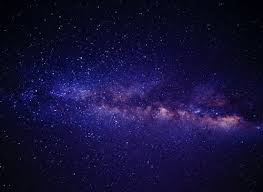
\includegraphics[scale=1]{Figures/universe}	
	\caption{Sample picture of universe }
	\label{fig:universe}
\end{figure}

These guidelines are provided to formally expose you to the various ethical and technical issues involved in writing up your work and the format you are required to adhere to while submitting your project report.
\end{comment}

\section[Motivation]{\textbf{Motivation}}
%% BEGIN CONTENT HERE
The motivation behind choosing this project stems from two persistent and interrelated challenges in the field of machine learning hardware: the need for energy-efficient, real-time ML execution platforms suitable for edge devices, and the growing importance of performing architectural exploration of FPGA platforms using established frameworks such as the widely adopted VTR toolchain, particularly in the context of ML-centric workloads.

As ML becomes increasingly embedded into devices like drones, sensors, wearables, and autonomous systems, the demand for compact, low-power hardware accelerators has intensified. General-purpose processors fall short due to their serial execution model, while GPUs — though powerful — are often unsuitable for power-sensitive environments. This made the case for exploring FPGAs, which offer flexibility and energy efficiency. However, the choice of FPGA internal architecture significantly impacts ML performance. The first part of the project involved evaluating existing FPGA architectures using the VTR toolchain. Architectures were assessed using adder tree and FIR filter benchmarks, which are representative of machine learning workloads due to their reliance on fundamental operations like addition and multiplication.

Simultaneously, in academic and applied research, Principal Component Analysis (PCA) remains a cornerstone of dimensionality reduction in ML and signal processing. Yet, very few hardware implementations efficiently support PCA operations like covariance matrix computation and eigendecomposition. This motivated the second part of the project — designing Manojavam, a domain-specific accelerator that performs PCA using custom RTL logic.

The idea of combining architectural benchmarking with the design of a complete hardware accelerator emerged as a powerful way to bridge theory and application. It allowed for deep exploration of both low-level FPGA features and high-level ML operations, and aligned well with current trends in edge AI and domain-specific hardware design.

\begin{comment}
Brief the motivation of selecting your project title. You can elaborate the challenges in the specific area, relevance and importance of the chosen topic. 
\end{comment}

\section[Problem statement]{\textbf{Problem statement}}
%% BEGIN CONTENT HERE
General-purpose processors are inherently inefficient for machine learning (ML) workloads due to their limited parallelism, sequential instruction execution, and high power consumption, while GPUs, though better suited for compute-intensive tasks, suffer from excessive energy usage and memory bandwidth constraints. Although FPGAs offer a promising balance of configurability, parallelism, and energy efficiency, current FPGA architectures are not optimized for ML tasks, particularly those involving low-precision arithmetic or approximate computing. At the same time, domain-specific accelerators capable of performing foundational ML algorithms like Principal Component Analysis (PCA) in an efficient and scalable manner are largely absent in RTL-level research and development. This project aims to address these challenges by conducting an architectural exploration of FPGA fabrics for ML workloads and designing a custom PCA accelerator, Manojavam, capable of efficient covariance matrix computation and eigendecomposition using systolic arrays and RTL-based optimization.

\begin{comment}
	Define the problem statement in this section, in one paragraph.
\end{comment}

\section[Objectives]{\textbf{Objectives}}
%% BEGIN TEXT HERE
The objectives of the project are-
\begin{enumerate}
	\item To explore and evaluate FPGA architectural features, specifically carry chain-based designs versus DSP block-based architectures, for their suitability in machine learning workloads using the VTR toolchain.
	\item To design and implement a domain-specific hardware accelerator named Manojavam for Principal Component Analysis (PCA), featuring matrix multiplication using systolic arrays and eigendecomposition using a custom Jacobian Unit.
	\item To synthesize, simulate, and validate the proposed accelerator on both FPGA and ASIC flows, and compare its performance with conventional CPU/GPU implementations as well as existing state-of-the-art PCA accelerators.
\end{enumerate}

\begin{comment}
The objectives of the project are
\begin{enumerate}
\item To design a pipelined ADC for audio frequency range
\item List all the objectives in the above format , starting with "To"
\item Limit the number of objectives to a maximum of three
\end{enumerate}
\end{comment}

\section[Literature Review]{\textbf{Literature Review}}
%% BEGIN CONTENT HERE
\subsection{Related Work on FPGA Architectural Exploration for ML Workloads}
Over the past three decades, the architecture of Field-Programmable Gate Arrays (FPGAs) has undergone extensive evolution, driven by the increasing complexity of target applications and advances in process technologies. A core objective of FPGA architecture research has been to balance flexibility with performance, area efficiency, and power consumption.

Initial FPGA designs employed basic logic elements (BLEs) consisting of small look-up tables (LUTs) and flip-flops. These BLEs were clustered into larger logic blocks with local interconnect to enhance packing efficiency and reduce inter-block routing delay. Ahmed and Rose\cite{ahmed2000effect} empirically studied the area-delay trade-offs of different LUT sizes and BLE clusterings, concluding that 4–6 input LUTs and cluster sizes of 3–10 BLEs provide an optimal area-delay product. Fracturable LUTs were introduced in Altera’s Stratix II\cite{stratix2007stratix} and Xilinx’s Virtex-5\cite{xilinxvirtex} to mitigate underutilization in large LUTs. These allowed a single 6-LUT to be decomposed into two 5-LUTs, improving logic density and enabling more effective packing of smaller functions.

Arithmetic operations—especially additions and multiplications—are central to many FPGA applications, from DSP to machine learning. Initially, such operations were implemented using LUTs, but this approach suffered from excessive logic utilization and long critical paths. To address this, modern FPGAs integrate hardened carry chains within their logic elements. Murray et al\cite{boutros2019math} found that 22\% of the logic elements in typical FPGA workloads implement arithmetic, justifying the need for specialized support. Their study shows that hardening carry chains improves performance by 75\% for arithmetic microbenchmarks and 15\% for general workloads.

The latest Intel Agilex devices\cite{intel_agilex_2020} and Xilinx Versal architecture\cite{xilinx_versal_trm_2021} further advance this trend by implementing carry-skip and carry-lookahead adders, respectively. The Agilex architecture hardens 2-bit carry-skip adders per logic element, enabling dense and high-speed arithmetic, while Versal enables 1-bit per logic element with advanced carry logic. Stratix devices also use fracturable 6-LUTs that support 2-bit arithmetic per adaptive logic module (ALM), achieving both compact area and high arithmetic throughput.

Proposals to enhance arithmetic density include logic elements with 4-bit carry chains arranged in single or dual configurations\cite{boutros2019math}\cite{boutros2021fpga}. These studies demonstrated that dual-chain configurations improve multiply-accumulate (MAC) operation density by up to 17\% and reduce area by 8\%, showing promise for arithmetic-intensive ML and DSP workloads.

A critical aspect of FPGA architecture research is evaluating trade-offs across area, timing, and power. The typical methodology involves defining an architecture model, selecting benchmark circuits, and utilizing a CAD toolchain to simulate implementation results\cite{boutros2021fpga}. The Verilog-to-Routing (VTR) tool\cite{rose2012vtr} is a widely used open-source CAD framework for this purpose. It allows researchers to model custom FPGA architectures through descriptive XML files, map benchmark designs, perform placement and routing, and obtain post-routing metrics. This methodology underpins much of the academic work in architecture exploration and was adopted in the present study for fair evaluation of different carry chain designs.

Benchmarking traditionally relied on the MCNC suite\cite{yang1991logic}, which includes small logic-centric designs. However, these are no longer representative of modern FPGA applications. The Titan benchmark suite\cite{rose2012vtr}, derived from industrial designs, provides larger and more realistic circuits and has become a standard in architecture evaluation. Other works have emphasized the need for emerging benchmark suites that better reflect ML and signal-processing-heavy workloads.

Modern commercial FPGAs have embraced increasing heterogeneity, incorporating DSP blocks, embedded memories, and even hardened interconnect pipelining. For example, Intel’s Stratix 10 integrates optional pipeline registers within routing drivers using configurable pulse latches\cite{intel_stratix10_2019}, while Xilinx Versal includes input-side block registers to reduce long interconnect delay\cite{xilinx_versal_trm_2021}. These additions aim to mitigate timing bottlenecks associated with deeper pipelining in high-performance workloads.

Additionally, attempts to repurpose the logic fabric for low-precision ML tasks, such as implementing 8-bit MACs using LUTs and carry chains\cite{boutros2021fpga}, have driven research into logic elements that better support partial product reduction and carry-propagation efficiency. Carry chains have proven useful in implementing tree-based multipliers and accumulators, underscoring their utility beyond addition.

\subsection{Related Work on PCA and SVD Accelerators}
There have been attempts to overcome computational challenges associated with Principal Component Analysis (PCA) and Singular Value Decomposition (SVD). As PCA and SVD are inherently related to each other, the below sections highlight the state of art approaches to accelerate both PCA and SVD workloads on high performance computing hardware. 

%%% All PCA Architecture Surveys
%\subsection{Principal Component Analysis (PCA) : Approaches and Architectures}

In \cite{pca_architecture-1}, the authors implement a full fledged accelerator for Principal Component Analysis, where the architecture solves both the learning and mapping phases. They implement eigenvalue decomposition using QR factorization with Givens CORDIC rotation on the computed covariance matrix. The accelerator works at an operational frequency of 183 MHz, and consumes 56\% of LUTs, 19\% of memory and 88\% of the DSP blocks, on a Xilinx Virtex-7 FPGA. However, the design does not scale well for large matrices and operates better than an Nvidia GPU and Intel processors for small matrices, with a maximum tested dimension of 16×30. The authors employ a parallel vector based matrix multiplication approach. 

A reconfigurable PCA accelerator was proposed in \cite{pca_architecture-2}, where the accelerator was employed to preprocess data from satellites to the ground in low bandwidth scenarios, saving them cost. The authors implemented an EVD engine, and used a DMA module with prefetching to hide latencies associated with memory bottlenecks. The architecture employs 67\% of the available FPGA resources, and shows a performance improvement of 10x and 12x on the AVIRIS Cuprite and Jasper datasets respectively. However, the chip does not accelerate matrix multiplication, and the authors claim that it consumes too much overhead, and works faster on software. Moreover, the key microarchitectural details about the Jacobi algorithm are not revealed. 

A full-fledged PCA accelerator was proposed in \cite{pca_architecture-3}, implementing both learning and mapping phases, designed entirely using High-Level Synthesis (HLS). The primary application of the accelerator is hyperspectral imaging, where it computes the covariance matrix of the input dataset using a Covariance Unit and performs Eigenanalysis through an SVD unit. However, the paper does not disclose specific microarchitectural details of these units. The design was implemented on two FPGA platforms: the Zynq-7000 XC7Z020CLG484-1 and the Virtex-7 XC7VX690TFFG1761-2, with reported power consumption of 2.376W and 9.786W, respectively. A notable drawback of the design is its reliance on HLS, which, while simplifying hardware development, abstracts away low-level optimizations that could improve efficiency and performance. 

An outlier detection scheme for Network Intrusion Detection Systems (NIDS) is proposed in \cite{pca_architecture-4}, leveraging Principal Component Analysis for anomaly detection after an initial Feature Extraction Module (FEM) processes the network traffic. The PCA framework follows a two phase approach : an offline PCA phase, where the principal components are obtained from a training dataset, and the online PCA phase, where the incoming data is projected onto these principal components to detect outliers in real time. The authors note that while PCA significantly reduces the computational complexity, eigenvector calculations and sorting remain sequential and difficult to parallelize, making them less suited for FPGA based acceleration. However, the principal component score calculations, which involve matrix to vector computations, are efficiently parallelized in hardware. 

A dynamic on-the-fly reconfigurable PCA accelerator was proposed in \cite{pca_architecture-5}, where the accelerator dynamically reconfigures itself during different stages of the PCA algorithm. The implementation was developed on the ML605 FPGA board, which is based on 40 nm CMOS technology and features a Xilinx Virtex-6 (XC6VLX240T-FF1156) FPGA, MicroBlaze soft processors, 2MB of on-chip BRAM, and 512MB of DDR3-SDRAM for large-scale data storage. The design was implemented using a mix of Verilog and VHDL and operates at a maximum clock frequency of 100 MHz. The authors employed a Covariance Unit to compute the covariance matrix efficiently and used QR factorization for Eigenvalue Decomposition (EVD). However, the paper does not provide microarchitectural details of these units. While dynamic reconfiguration led to a 71\% area savings, it introduced significant reconfiguration overheads in the order of milliseconds, which could degrade overall performance. Additionally, the authors note that while the cyclic Jacobi method is effective for small matrices, alternative methods such as QR or Householder decomposition may be better suited for larger matrices.

%%% All SVD Architecture Surveys
%\subsection{Singular Value Decomposition (SVD) : Approaches and Architectures}

The work in \cite{svd_architecture-1} proposes an FPGA accelerator for Singular Value Decomposition employing fixed point arithmetic, using the Hestenes-Jacobi algorithm and CORDIC. The accelerator works at an operational frequency of 250 MHz on a Xilinx Kintex-7 XC7K325T FPGA. It achieves a speedup between 8.5× and 15.3× over MATLAB and between 2.1× and 6.3× over GPU implementations. However, the design is not scalable to very large matrices due to block RAM limitations, and the authors suggest that an array of FPGAs may be needed for handling larger matrices beyond 128×128. 

An FPGA based accelerator for both Singular Value Decomposition and Eigenvalue Decomposition is proposed in \cite{svd_architecture-2}, where the accelerator is optimized for real time performance. The accelerator is based on the Jacobi algorithm, employing the Brent-Luk systolic array to efficiently compute SVD, and using CORDIC based algorithm for EVD. The design, when dumped on the Xilinx Virtex-5 FPGA, operates at a frequency of 130 MHz, and shows a performance improvement of 4x compared to a 2.53 GHz Intel processor, and an improvement of 2x for EVD when compared to the previous FPGA based designs. The hardware utilization for an 8×8 matrix reaches 98\%, but while this demonstrates high efficiency, the increasing resource demand for larger matrices may impact scalability. 

The work in \cite{svd_architecture-3} proposes an SVD engine, designed on 90nm CMOS technology, wth an operational frequency of 101.2 MHz and a power of 125 mW, for very high throughput MIMO-OFDM systems. The authors implemented an adaptive SVD engine, which would dynamically modify the output eigenvectors and values with changes in inputs. An Orthogonal Reconstruction (OR) scheme is also implemented to correct errors due to fixed point arithmetic, ensuring very high accuracy. However, the SVD engine primarily relies on a sequential execution model, particularly in Jacobi-based updates and CORDIC-based rotations, which may limit scalability for larger matrices beyond 4×4. 

The work in \cite{svd_architecture-4} compares and contrasts the execution of the Jacobi algorithm on the CPU, GPU, and FPGA, revealing that the GPU suffers from performance degradation due to unstructured global memory access patterns. To address this, the paper proposes three enhanced memory access patterns—Modified Access (MA), Symmetric Access (SA), and Maximum Coalesced Access (MCA)—which significantly improve GPU performance. The study highlights the critical role of memory access optimization in accelerating the Jacobi algorithm, particularly for GPU implementations, while also confirming that FPGA outperforms both GPU and CPU in overall efficiency for eigenanalysis. 

The work in \cite{svd_architecture-5} proposes a parallel fast-converging Jacobi algorithm designed for larger matrices, improving upon traditional Jacobi-based methods. Instead of processing elements in a fixed order, the algorithm selects N/2 of the largest off-diagonal elements in each iteration while maintaining row-column exclusivity. This reduces the number of Jacobi sweeps required and accelerates convergence. The design employs CORDIC-based rotations for efficient computation of trigonometric functions and is implemented on the Xilinx Virtex-6 XCVLX365T FPGA. Although the engine introduces an optimized Jacobi approach, it does not include a dedicated matrix multiplication accelerator to enhance intermediate transformations within the algorithm. As a result, row and column updates rely solely on DSP-based multipliers, which may introduce computational bottlenecks for larger matrices. Integrating a matrix multiplication accelerator (such as a systolic array or TPU-like cores) could further improve the throughput and scalability of the SVD core, especially for matrices beyond 32×32. 

A Hestenes-Jacobi processor for SVD was developed in \cite{svd_architecture-6}, which computed SVD for arbitrary size matrices in IEEE-754 double precision floating point format. The architecture comprised three dedicated units : the Hestenes Preprocessor, Jacobi Rotation unit and the Update unit. The authors do not employ a systolic array for matrix multiplication, noting that traditional systolic architectures are optimized for square matrices. However, the paper neither explores nor considers alternative approaches such as block-streaming systolic architectures, which could potentially improve efficiency in rectangular matrix multiplications. The design was dumped on a Xilinx Virtex-5 XC5VLX330 FPGA, operating on 150 MHz, consuming 89\% LUTs, 91\% BRAMs and 53\% DSPs. Matrices of dimension in the order of 1024 were tested successfully. However, they employ Xilinx Coregen IPs in their design, consuming 9, 14, 57 and 57 clock cycles for multiplier, adder-subtractor, divider and square root blocks respectively. 


\begin{comment}
A literature review is a text of a scholarly paper, which includes the current knowledge including substantive findings, as well as theoretical and methodological contributions to a particular topic. Literature reviews are secondary sources, and do not report new or original experimental work. Most often associated with academic-oriented literature, such reviews are found in academic journals, and are not to be confused with book reviews that may also appear in the same publication. Literature reviews are a basis for research in nearly every academic field . A narrow-scope literature review may be included as part of a peer-reviewed journal article presenting new research, serving to situate the current study within the body of the relevant literature and to provide context for the reader. In such a case, the review usually precedes the methodology and results sections of the work.

\subsection{Sample}
The main types of literature reviews are: evaluative, exploratory, and instrumental. A fourth type, the systematic review, is often classified separately, but is essentially a literature review focused on a research question, trying to identify, appraise, select and synthesize all high-quality research evidence and arguments relevant to that question. A meta-analysis is typically a systematic review using statistical methods to effectively combine the data used on all selected studies to produce a more reliable result.
\subsubsection[Review types]{\textbf{Review types}}

The main types of literature reviews are: evaluative, exploratory, and instrumental. A fourth type, the systematic review, is often classified separately, but is essentially a literature review focused on a research question, trying to identify, appraise, select and synthesize all high-quality research evidence and arguments relevant to that question. A meta-analysis is typically a systematic review using statistical methods to effectively combine the data used on all selected studies to produce a more reliable result.


\subsubsection[Process and product]{\textbf{Process and product}}

Distinguish between the process of reviewing the literature and a finished work or product known as a literature review. The process of reviewing the literature is often ongoing and informs many aspects of the empirical research project. All of the latest literature should inform a research project. Scholars need to be scanning the literature long after a formal literature review product appears to be completed.

\subsubsection{\textbf{Page limitation}}

A careful literature review is usually 15 to 30 pages and could be longer. The process of reviewing the literature requires different kinds of activities and ways of thinking and link the activities of doing a literature review with Benjamin Bloom’s revised taxonomy of the cognitive domain (ways of thinking: remembering, understanding, applying, analysing, evaluating, and creating).

This section should contain the review of the literature in the past.You should review a minimum of 10 papers from standard reference journals. Kindly avoid local conference papers and papers from predatory journals. Kindly consult with your guide and finalize papers to be considered for review before adding in this section.Report the major observations and findings from each paper in one paragraph in the format given below.

 proposed various techniques for adders and multipliers.Add the reference papers to the bibliography section using Jabref and cite it here using the instructions given in further chapters.


\subsubsection{\textbf{Plagiarism}}

To use someone else's exact words without quotation marks and appropriate credit, or to use the unique ideas of someone else without acknowledgement, is known as plagiarism. In publishing, plagiarism is illegal; in other circumstances, it is, at the least, unethical. You may quote or paraphrase the words or ideas of another if you document your source. Although you need not enclose the paraphrased material in quotation marks, you must document the source. 

Paraphrased ideas are taken from someone else whether or not the words are identical. Paraphrasing a passage without citing the source is permissible only when the information paraphrased is common knowledge in a field. (Common knowledge refers to historical, scientific, geographical, technical, and other type of information on a topic readily available in handbooks, manuals, atlases and other references). 

\subsubsection{How to add Reference}
Use \texttt{Jabref} which will help in adding the reference in a separate file, from which one can use \verb|\citep\{\}| command to add reference. A sample, referring to a textbook would look something like this,\cite{Razavi2000}.
\end{comment}

\section[Brief Methodology of the project]{\textbf{Brief Methodology of the project}}
%% BEGIN CONTENT HERE
The methodology followed in this project combines architectural benchmarking and accelerator design to address both the evaluation and implementation aspects of efficient ML hardware. The workflow begins with the selection of benchmark circuits relevant to ML workloads — such as adder trees and FIR filters — which are then mapped onto different FPGA fabric configurations using the VTR toolchain. These include single and double carry chain-based architectures and DSP-centric designs. Performance metrics such as delay, logic utilization, and power are recorded to identify trends and architectural advantages. Fig.\ref{fig:vtr_methodology} outlines the methodology of the FPGA architectural exploration.

\begin{figure}[htbp]
	\centering
	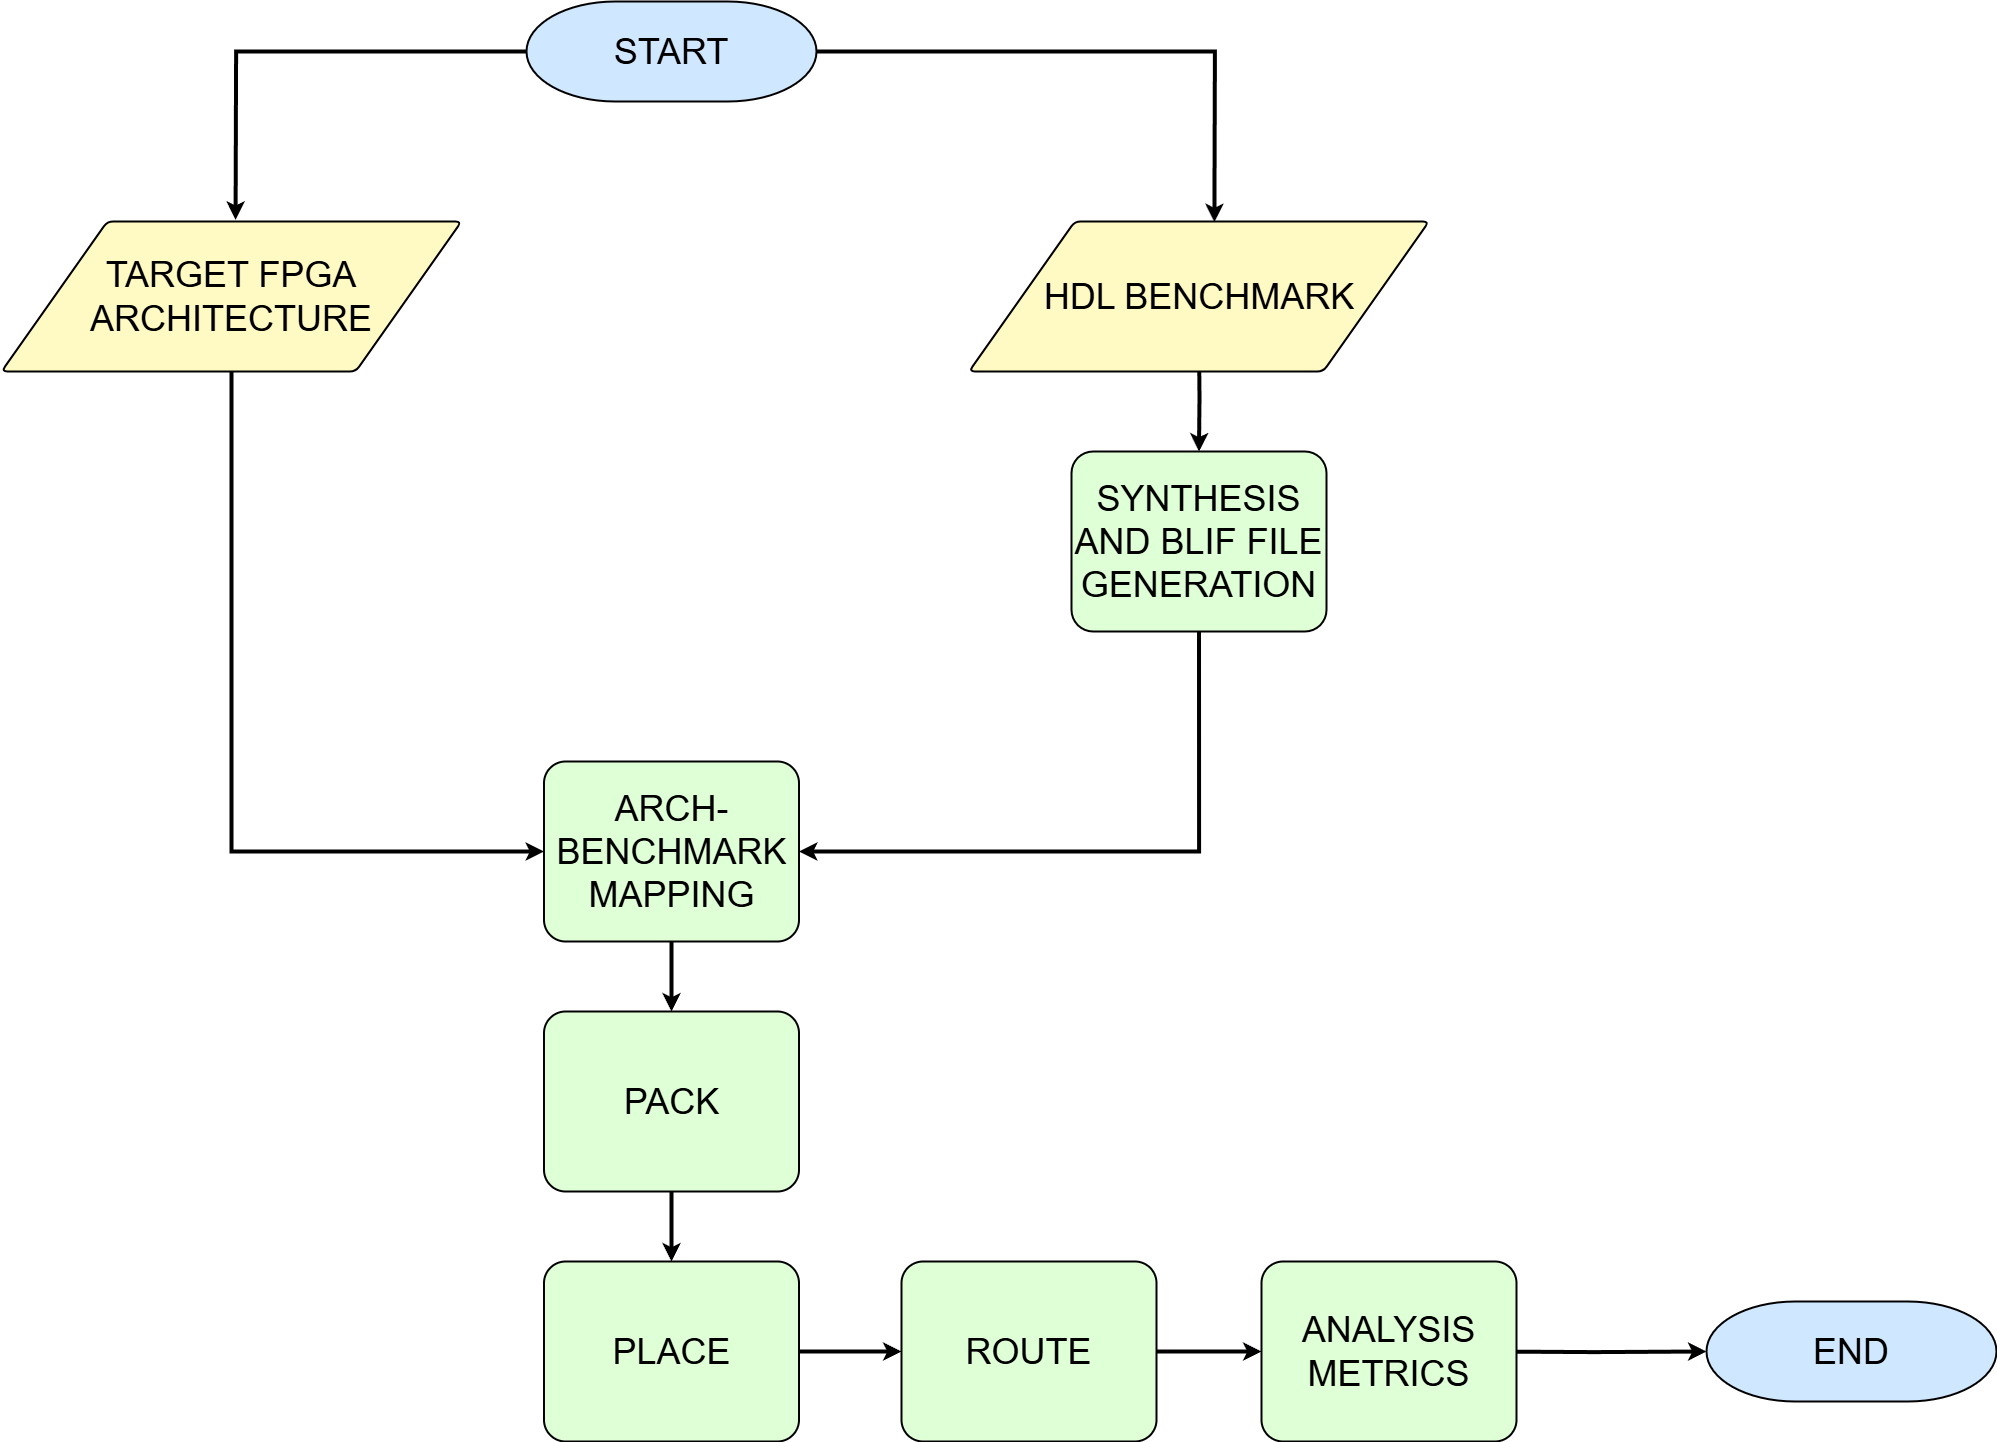
\includegraphics[scale=0.225]{Figures/VTR_Methodology_v2.png}	
	\caption{Methodology of FPGA Architectural Exploration}
	\label{fig:vtr_methodology}
\end{figure}

Parallelly, a domain-specific accelerator named Manojavam is developed using a modular RTL design. It comprises 8 systolic arrays for matrix multiplication, a novel Jacobian Unit for SVD-based eigendecomposition, and a structured cache system. RTL design and simulation are performed using Vivado for FPGA flow, while ASIC design is carried out using the OpenLane toolchain. Floorplanning, timing closure, and power analysis are conducted to validate the feasibility of deployment. The performance of Manojavam is then compared against CPU, GPU, and existing PCA accelerator implementations using a custom-built simulator and various matrix input sizes. The methodology for the design of Manojavam is highlighted in Fig.\ref{fig:manojavam_methodology}.

\begin{figure}[htbp]
	\centering
	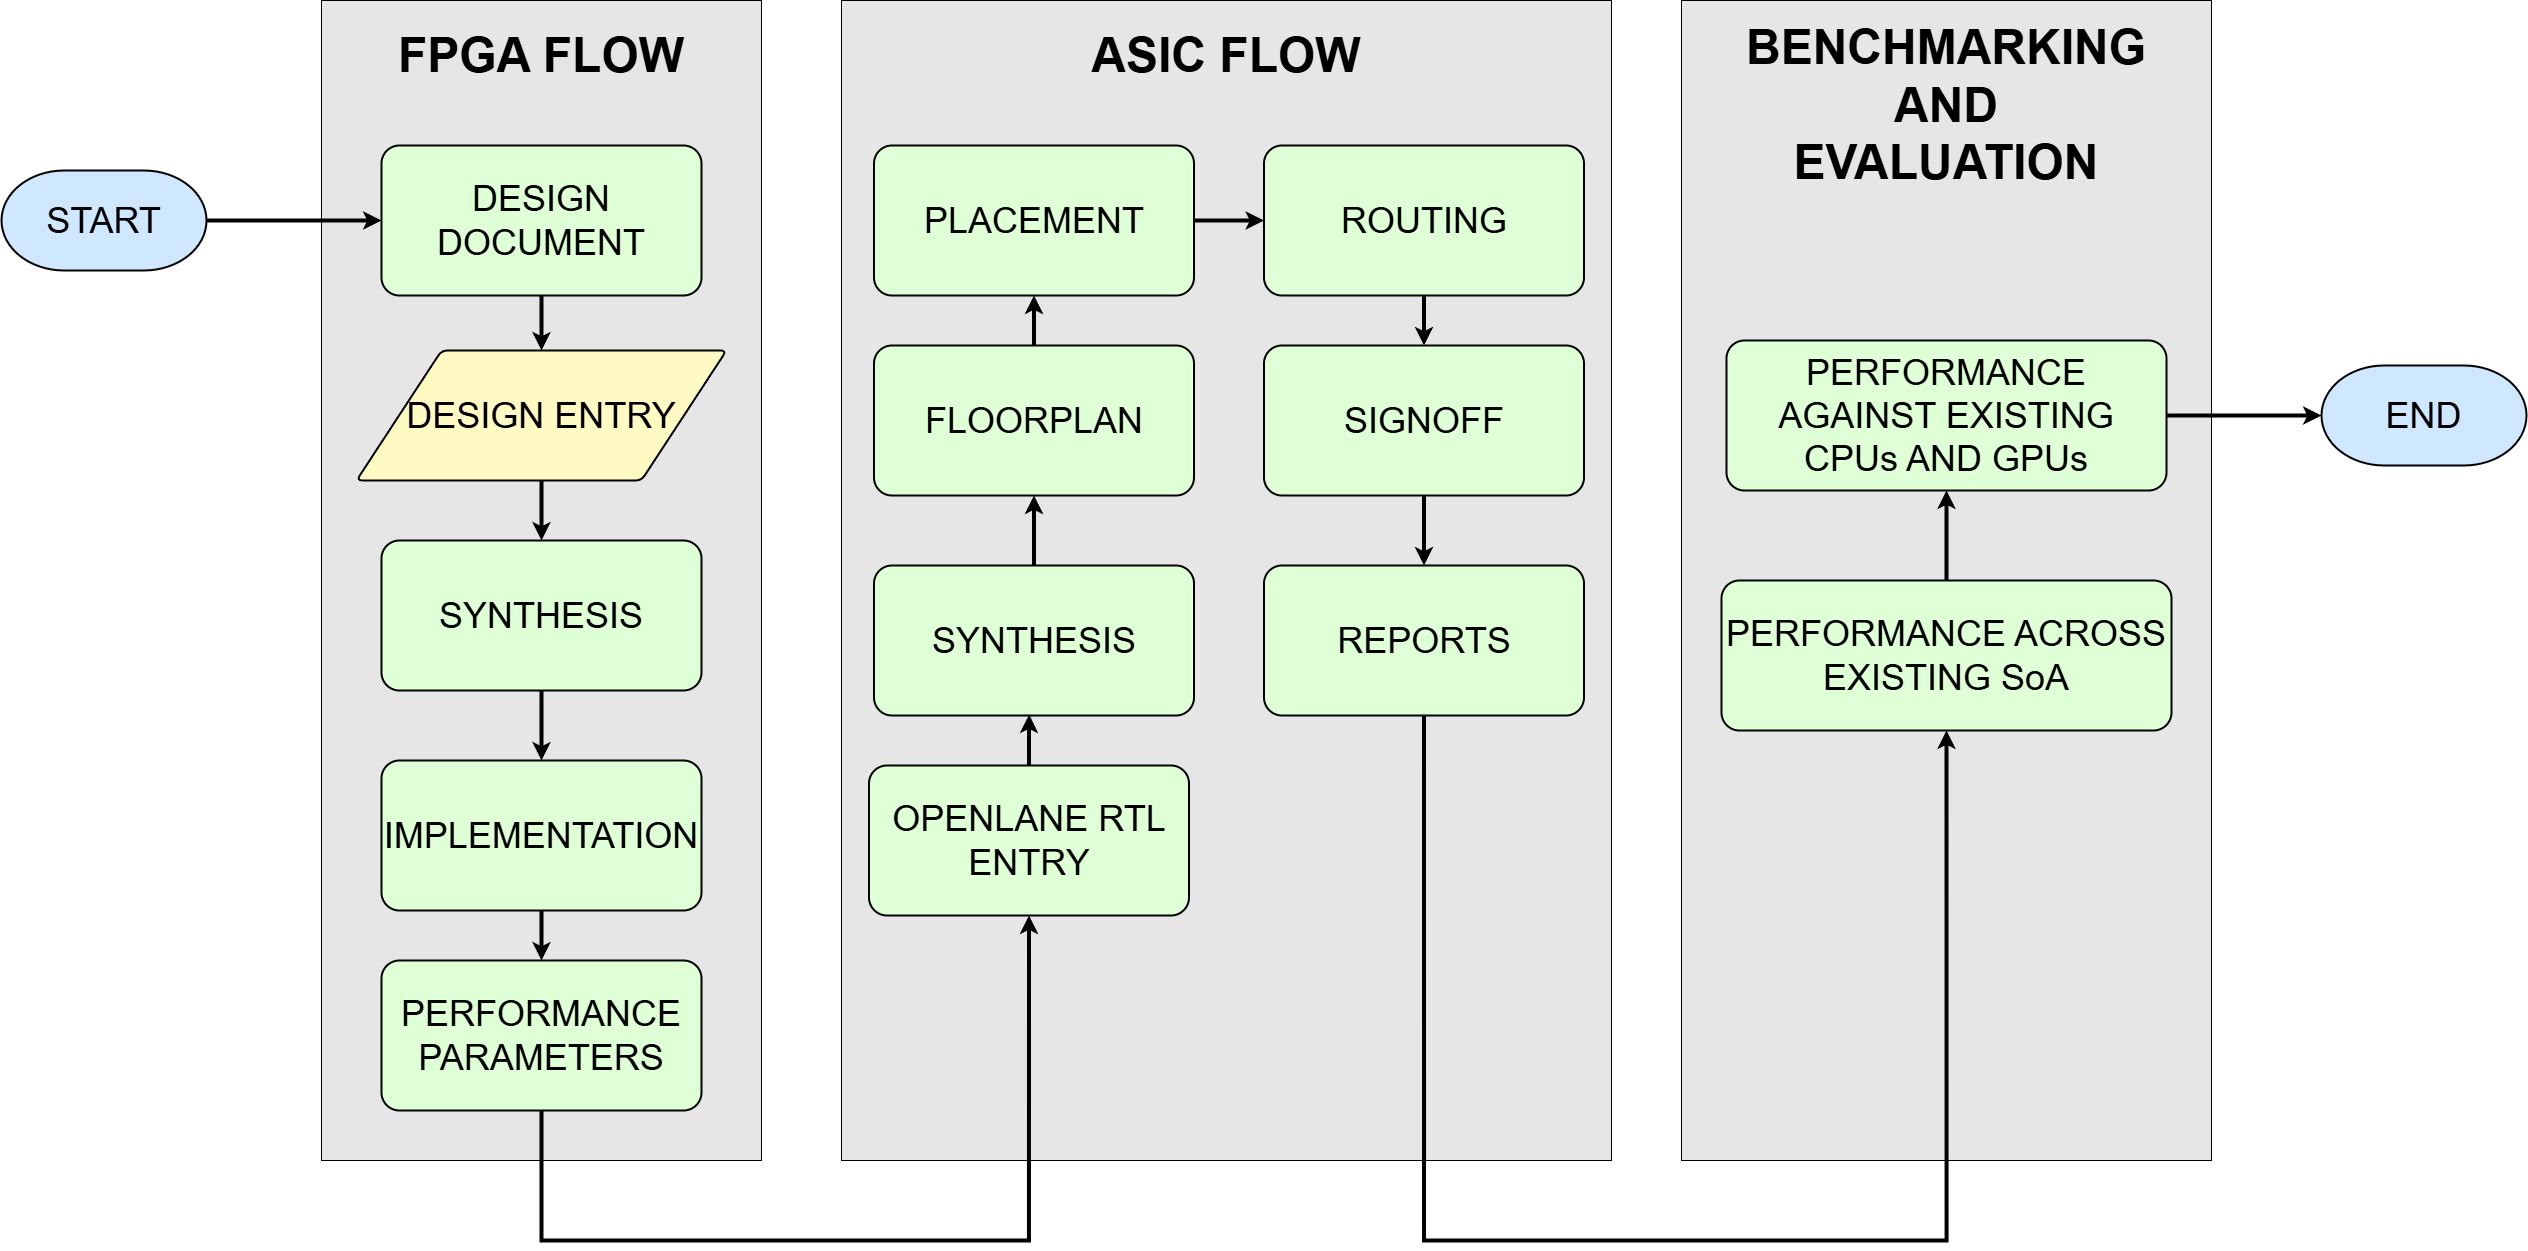
\includegraphics[scale=0.195]{Figures/manojavam_methodology_v2.png}
	\caption{Methodology for Manojavam Accelerator Development}
	\label{fig:manojavam_methodology}
\end{figure}

\begin{comment}
Discuss about the methodology you identified to execute the objectives of your project in brief. Methodology is a system of practices, techniques, procedures, and rules used to execute a particular project. You can elaborate the methodology in a later chapter. Here you can present in the form of a flow diagram and explain the methodology in a paragraph.
\end{comment}

\begin{comment}
\section[Assumptions made / Constraints of the project]{\textbf{Assumptions made / Constraints of the project}}

List the assumptions made for the execution of the project in this section. You can also elaborate on the major constraints of the project. This section should clearly state under what conditions your project is valid. It is mandatory to have this section in your project report.
\end{comment}

\section[Organization of the report]{\textbf{Organization of the report}}

This report is organized as follows. 
\begin{itemize}
\item Chapter 2 discusses the fundamentals and foundational knowledge of FPGA architectures and domain specific acceleration.
\item Chapter 3 discusses the design methodology.
\item Chapter 4 discusses the implementation strategies of both projects.
\item Chapter 5 discusses the results and discussions.
\item Chapter 6 discusses the conclusions and future scope of work.
\end{itemize}

.

%Chapter 2
\chapter{Theoretical Foundations and Technical Prerequisites}
%% BEGIN CONTENT HERE
An in-depth understanding of architectural design principles, matrix operations, and toolchains is essential for developing high-performance ML hardware. This chapter outlines the foundational concepts required to carry out FPGA architectural exploration using the VTR toolchain and to design the domain-specific PCA accelerator, Manojavam. It begins by covering FPGA architecture types relevant to ML applications, followed by essential matrix computation techniques and PCA formulations. The chapter also introduces key tools such as VTR, Vivado, OpenLane, and CACTI, which were instrumental in modeling, implementing, and evaluating the proposed designs.


\begin{comment}
From Chapter 2 onwards, every chapter should start with an introduction paragraph. This paragraph should brief about the flow of the chapter. This introduction can be limited within 4 to 5 sentences. The chapter heading should be appropriately modified (a sample heading is shown for this chapter).But don't start the introduction paragraph in the chapters 2 to end with "This chapter deals with....". Instead you should bring in the highlights of the chapter in the introduction paragraph.
\end{comment}
%% START OF THE SECTION - FUNDAMENTALS OF FPGA ARCHITECTURE %%
\section{Fundamentals of FPGA Architecture}
%% BEGIN CONTENT HERE
Field-Programmable Gate Arrays (FPGAs) are a class of integrated circuits that provide post-fabrication reconfigurability at the hardware level. Unlike fixed-function ASICs (Application-Specific Integrated Circuits), FPGAs can be programmed to implement any digital logic circuit by configuring a rich array of programmable logic blocks, interconnects, and embedded hard blocks. This section provides an in-depth exploration of the foundational architecture of FPGAs, with a focus on the key structural elements and their evolution. Fig.\ref{fig:fpga architecture} highlights the early v/s modern style FPGA blocks that integrate many hardblocks on the fabric.

\begin{figure}
	\centerline{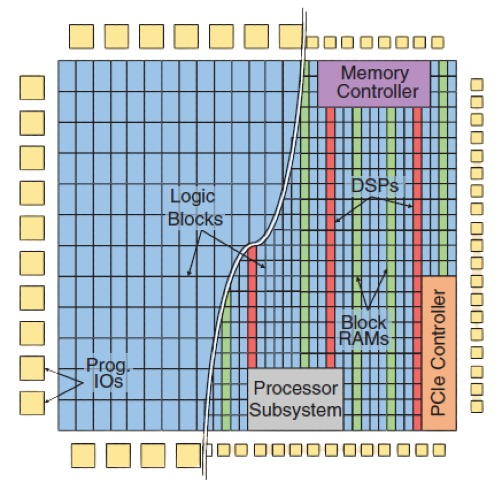
\includegraphics[scale = 0.6]{Figures/fpga_architecture.jpg}}
	\caption{FPGA Architecture Overview : Early v/s Modern\cite{boutros2021fpga}}
	\label{fig:fpga architecture}
\end{figure}

\subsection{Configurable Logic and Logic Clusters}
The smallest unit of computation in an FPGA is the Basic Logic Element (BLE), which typically comprises a K-input Lookup Table (K-LUT), a flip-flop (FF), and multiplexers to select between combinational and registered outputs. The K-LUT is a truth table stored in SRAM that can implement any K-input Boolean function. For example, a 6-LUT can encode any 6-input logic by programming 64 SRAM bits. Fig.\ref{fig:4-lut transistor} depicts the implementation of a 4-LUT at a transistor level.

\begin{figure}
	\centerline{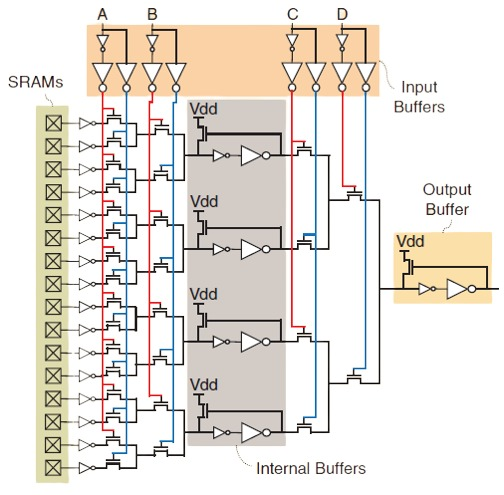
\includegraphics[scale = 0.6]{Figures/4-LUT-Transistor.jpg}}
	\caption{Transistor Implementation of a 4-LUT\cite{boutros2021fpga}}
	\label{fig:4-lut transistor}
\end{figure}

Modern BLEs implement fracturable logic to increase logic packing efficiency\cite{funda-fpga-arch-1}. A fracturable 6-LUT can operate as either a single 6-input LUT or two 5-input LUTs sharing inputs\cite{stratix2007stratix}. This flexibility reduces unused logic and enables higher performance. Intel's Adaptive Logic Modules (ALMs) and Xilinx's slice-based architectures exemplify this trend, enabling efficient use of logic resources.

BLEs are grouped into larger clusters called Logic Array Blocks (LABs) or Configurable Logic Blocks (CLBs). Each LAB may contain 8 to 32 BLEs and includes a local interconnect network for intra-block communication. This local interconnect is typically implemented using multiplexers arranged as full or partial crossbars\cite{funda-fpga-arch-2}\cite{funda-fpga-arch-3}. As the number of BLEs per LAB increases, more signal routing can be localized, reducing pressure on global routing resources and improving performance. The internal architecture of the LAB is given in Fig.\ref{fig:lab internal architecture}.

\begin{figure}
	\centerline{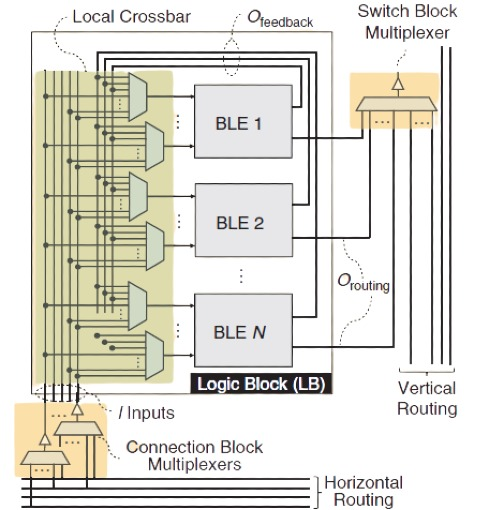
\includegraphics[scale = 0.6]{Figures/LAB-architecture.jpg}}
	\caption{LAB Internal Architecture\cite{boutros2021fpga}}
	\label{fig:lab internal architecture}
\end{figure}

The design trade-off in LAB size lies between logic utilization, routing efficiency, and critical path delay. Larger LABs reduce inter-block communication but increase complexity in placement and delay modeling.

\subsection{Programmable Routing Architecture}
The dominant routing style in modern FPGAs is the island-style architecture. In this topology, logic blocks (LABs) are arranged in a 2D grid and are surrounded by horizontal and vertical routing channels. These channels consist of wire segments of varying lengths and programmable switches.

Three main elements define the island-style routing fabric:
\begin{enumerate}
	\item \textbf{Connection Blocks:} Interface logic block I/Os to routing channels.
	\item \textbf{Switch Blocks:} Enable programmable interconnection between horizontal and vertical wires.
	\item \textbf{Wire Segments:} Allow signal propagation across the chip, often spanning 1, 4, or 16 logic blocks.
\end{enumerate}

Efficient switch block designs (e.g., Wilton pattern) and wire-length tuning reduce signal delay and area overhead\cite{funda-fpga-arch-4}. To address long-distance routing delays, modern FPGAs also employ hierarchical wiring and segment-bypassing strategies. The most popular routing style architecture, the island style routing architecture, is depicted in Fig.\ref{fig:island style routing architecture}. This style of routing is employed in the test architectures employed in the study, which we will see in the following sections.

\begin{figure}[H]
	\centerline{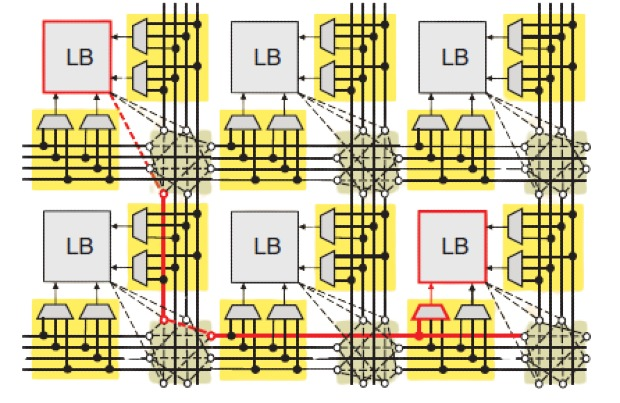
\includegraphics[scale = 0.6]{Figures/island_style_routing-removebg-preview.jpg}}
	\caption{Island Style Programmable Routing Architecture\cite{boutros2021fpga}}
	\label{fig:island style routing architecture}
\end{figure}

Programmable switches form the core of reconfigurable routing. Early designs used simple pass transistors, but these incur high resistance and delay\cite{funda-fpga-arch-5}. Buffered multiplexers are now preferred, where multiple pass transistors feed a buffer, improving speed and electrical isolation\cite{funda-fpga-arch-6}\cite{funda-fpga-arch-7}. This design limits signal injection points but significantly enhances signal integrity and performance.

\subsection{Embedded Arithmetic and Carry Chains}
Arithmetic operations such as addition and multiplication are common in FPGA workloads. Although they can be implemented with LUTs, this approach is inefficient. Instead, modern FPGAs integrate hardened arithmetic logic like carry chains directly within BLEs.

Carry chains enable fast ripple-carry and carry-skip adders. They allow the carry-out of one BLE to directly feed the carry-in of the next without passing through the general routing fabric, minimizing delay. Xilinx FPGAs use carry look-ahead logic in Versal devices, whereas Intel’s Agilex architecture implements two-bit arithmetic per logic element. These dedicated structures are optimized for speed and minimize logic usage for arithmetic-heavy workloads.

Advanced carry-chain structures like carry-skip and carry-lookahead adders are hardened to further accelerate arithmetic paths. Carry logic is commonly coupled with sum and propagate generation logic inside LUTs, and is tightly integrated into the physical layout to reduce interconnect delay. These carry networks are also exploited to accelerate custom DSP-style operators and are essential for low-precision multiply-accumulate (MAC) implementations.

These features are especially beneficial for domains requiring high arithmetic intensity, such as digital signal processing, image processing, and machine learning accelerators.

\subsection{On Chip Memory: BRAM and LUT-RAM}
To address diverse memory needs, FPGAs embed Block RAMs (BRAMs) with configurable size, depth, and access ports\cite{funda-fpga-arch-8}\cite{funda-fpga-arch-9}. A typical dual-port BRAM includes row/column decoders, sense amplifiers, and output multiplexers. Capacities range from 2Kb to 20Kb, with typical configurations supporting 1R/1W or 2R/W modes.

Peripheral logic allows BRAMs to operate in various data widths and depths (e.g., 32x64-bit or 64x32-bit)\cite{funda-fpga-arch-10}\cite{funda-fpga-arch-11}. Input/output ports are pipelined to ease timing closure, and routing interfaces are carefully optimized to reduce area and delay.

In addition to BRAMs, FPGA vendors allow LUTs to function as small distributed RAMs. By configuring LUT truth tables and adding minimal write logic, logic blocks can operate as single or dual-port LUT-RAMs (e.g., 64x10-bit). This memory is ideal for register files and coefficient storage. However, only a subset of logic blocks typically supports LUT-RAM to balance area cost\cite{funda-fpga-arch-12}.

\subsection{DSP Hard Blocks}
FPGAs embed hardened Digital Signal Processing (DSP) slices to accelerate multiply-accumulate (MAC) operations. These slices support pre-adders, multipliers, accumulators, and configurable pipelining\cite{funda-fpga-arch-13}. MACs can be cascaded to implement dot products, convolution, and matrix multiplications efficiently.

DSP slices reduce logic utilization and boost performance for compute-intensive tasks such as deep learning inference, FFTs, and image processing. 

\subsection{Programmable IO Blocks}
IOBs are specialized blocks that manage communication between the FPGA core and external devices. They support a wide range of electrical standards (e.g., LVCMOS, SSTL, LVDS) and features like:
\begin{enumerate}
	\item Programmable drive strength and slew rate
	\item On-die termination
	\item Programmable delay lines
	\item Differential signaling and serial transceivers
\end{enumerate}

Advanced IOs integrate DDR memory controllers and serial links (e.g., PCIe, Ethernet) with hardened logic. FPGA IOs are grouped into banks, each operating at configurable voltages. These features make FPGAs ideal for communication-heavy applications.

%% END OF THE SECTION - FUNDAMENTALS OF FPGA ARCHITECTURE %%

%% START OF THE SECTION - TARGET FPGA ARCHITECTURES USED IN THE STUDY %%
\section{Target FPGA Architectures Used in the Study}
This study explores and benchmarks three FPGA target architectures, each modeled using VTR (Verilog-to-Routing) XML architecture description files. These include: (1) an Intel Stratix-10-like architecture that serves as a high-performance, industry-grade baseline, and two custom arithmetic-optimized variants, namely (2) a 4-bit Single Carry Chain architecture and (3) a 4-bit Double Carry Chain architecture. Each design showcases unique internal arithmetic structures and carry chain implementations aimed at evaluating low-precision arithmetic performance, relevant to domains such as deep learning inference.

\subsection{Intel Stratix-10-like Architecture}
The Stratix-10-like architecture models a high-end commercial FPGA design. The logic fabric consists of Logic Array Blocks (LABs), each comprising 10 Adaptive Logic Modules (ALMs). Every ALM contains a 6-input Lookup Table (6-LUT) that is fracturable into two 5-LUTs, supporting rich logic packing. Each ALM exposes 8 input pins and 4 output pins, which may be optionally registered using internal flip-flops\cite{target-arch-1}. Fig.\ref{fig:stratix-10 block diagram} highlights the block diagram of Intel's Stratix-10 high level block diagram.

\begin{comment}
\begin{figure}[H]
	\centerline{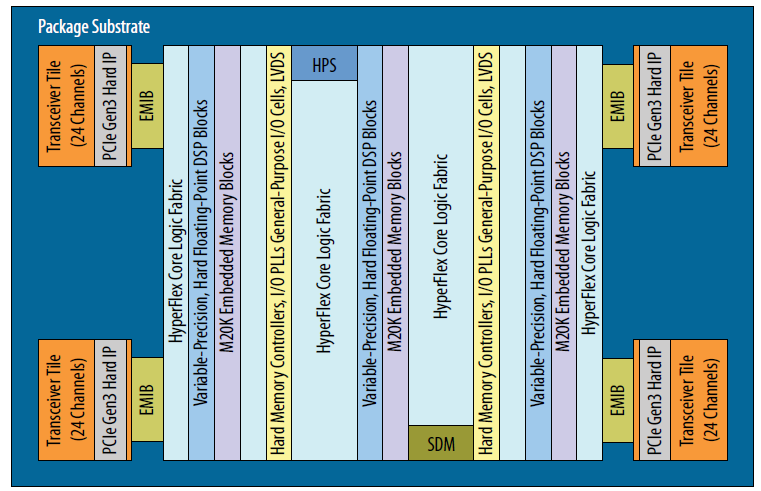
\includegraphics[scale = 0.60]{Figures/stratix_10_blockdiagram.png}}
	\caption{Intel's Stratix-10 Block Diagram}
	\label{fig:stratix-10 block diagram}
\end{figure}
\end{comment}

The key features of the Intel Stratix-10 like architecture are-
\begin{enumerate}
	\item \textbf{Arithmetic Mode Support:} Each 5-LUT can be fractured into two 4-LUTs, enabling two bits of addition per ALM in arithmetic mode. Thus, a LAB can support 20 bits of addition in a single carry chain across 10 ALMs.
	\item \textbf{Single Carry Chain:} The carry chain is linear, spanning the 10 ALMs within a LAB. The carry-out ($cout$) of one ALM feeds directly into the carry-in ($cin$) of the next, enabling fast arithmetic accumulation. 
	\item \textbf{Direct Connections:} ALM outputs feed both into neighboring LABs (left and right) and back into the LAB’s own input ports. This enhances localized reuse and dataflow.
	\item \textbf{Memory Support:} Each LAB can interface with a 20 Kb embedded RAM block, configurable in multiple true and simple dual-port modes.
	\item \textbf{DSP Integration:} A 27x27 DSP block (fracturable into 18x19 blocks) is embedded within the tile grid to support high-throughput MAC operations.
\end{enumerate}

This architecture balances general-purpose logic density with specialized arithmetic acceleration, making it suitable as a benchmark for more customized variants.

\subsection{4-bit Single Carry Chain Architecture}
This custom architecture builds on the Stratix-10 baseline but modifies the arithmetic capabilities for enhanced support of low-precision adders. It retains the same LAB structure—10 ALMs per LAB, 6-LUTs fracturable into two 5-LUTs—but introduces further fracturing into 3-LUTs\cite{target-arch-2}.

Key features of this architecture include-
\begin{enumerate}
	\item \textbf{Enhanced Arithmetic Fracturing:} In half the ALMs (ALM[0] to ALM[4]), each 5-LUT can be split into two 4-LUTs, and each 4-LUT further into two 3-LUTs. This yields 8 effective 3-LUTs per ALM, supporting 4-bit adders per ALM.
	\item \textbf{Single Carry Chain:} A single carry chain spans only the first 5 ALMs (ALM[0] to ALM[4]), providing a total of 20 bits of low-precision addition per LAB.
	\item \textbf{Optimized for Compact Arithmetic:} This configuration allows dense packing of small adders using minimal resources, reducing delay and improving energy efficiency for small-scale DSP and ML operations.
\end{enumerate}

This design evaluates how resource utilization and delay scale when packing narrow adders and embedding a shallow carry propagation chain.

\subsection{4-bit Double Carry Chain Architecture}
Expanding upon the single-chain variant, this architecture introduces a dual carry chain structure to exploit parallelism in arithmetic computation\cite{target-arch-2}.

Key features of this architecture include-
\begin{enumerate}
	\item \textbf{Double Carry Chains:} The LAB is split into two independent carry chains:
	\begin{itemize}
		\item Chain 1 spans ALM[0] to ALM[4]
		\item Chain 2 spans ALM[5] to ALM[9]
	\end{itemize}
	\item Each chain operates independently, with separate $cin$ and $cout$ ports, enabling concurrent execution of two 4-bit addition operations.
	\item \textbf{Full Arithmetic Fracturing:} Similar to the single chain, each ALM supports decomposition into eight 3-LUTs, enabling 4-bit addition within a compact area.
	\item \textbf{Routing Considerations:} The architecture includes direct interconnects between the carry-out of one LAB and the carry-in of the LAB below for each chain, supporting vertical propagation of arithmetic results.
\end{enumerate}

This configuration is ideal for evaluating parallelism vs. resource duplication trade-offs, particularly in scenarios where low-precision arithmetic operations can be concurrently dispatched, such as SIMD-style ML workloads.

\subsection{Summary of Architectural Differences}
Table.\ref{tab:fpga architectural differences between test architectures} summarizes the architectural differences between the Intel Stratix-10-like, 4-bit single carry chain and 4-bit double carry chain architectures.
% TABLE TO PRESENT THE ARCHITECTURAL DIFFERENCES
\begin{comment}
\begin{table}[ht]
	\centering
	\fontsize{10}{12}\selectfont
	\caption{FPGA Architectural Differences between Test Architectures}
	\scalebox{0.65}{
		\begin{tabular}{|c|c|c|c|}
			\hline
			\textbf{Feature} & \textbf{Stratix-10-like} & \textbf{4-Bit Single Chain} & \textbf{4-Bit Double Chain}\\
			\hline
			%\hline
			ALMs per LAB & 10 & 10 & 10 \\
			\hline
			Fracturable LUT Structure & 6-LUT to 5-LUT to 4-LUT & 6-5-4-3 LUT (half ALMs) & 6-5-4-3 LUT (all ALMs) \\
			\hline
			Carry Chains & 1 full LAB wide & 1 in ALM[0] to ALM[4] & 2 (ALM[0-4] and ALM[5-9]) \\
			\hline
			Arithmetic Parallelism & Sequentual & Narrow Serial (5 ALMs) & Dual Parallel Chains \\
			\hline
			Target Use-Case & General Logic and DSP & Low Precision MACs & Parallelized Arithmetic \\
			\hline
	\end{tabular}}
	
	%\label{tab:fpga architectural differences between test architectures}
\end{table}
\end{comment}

\begin{table}[htb]
	\fontsize{10}{12}\selectfont
	\caption{FPGA Architectural Differences between Test Architectures}
	\label{tab:fpga architectural differences between test architectures}
	\begin{tabular}{|p{3cm}|c|c|c|}
		%\hline
		%\multicolumn{4}{|c|}{Country List} \\
		\hline
		\textbf{Feature}& \textbf {Stratix-10-Like} & \textbf {4-Bit Single Chain} & \textbf{4-Bit Double Chain}\\
		\hline
		ALMs per LAB & 10 & 10 & 10\\\hline
		Fracturable LUT Structure & 6-LUT to 5-LUT to 4-LUT & 6-5-4-3 LUT (half ALMs) & 6-5-4-3 LUT (all ALMs) \\\hline
		Carry Chains & 1 full LAB wide & 1 in ALM[0] to ALM[4] & 2 (ALM[0-4] and ALM[5-9]) \\\hline
		Arithmetic Parallelism & Sequentual & Narrow Serial (5 ALMs) & Dual Parallel Chains \\\hline
		Target Use-Case & General Logic and DSP & Low Precision MACs & Parallelized Arithmetic \\\hline
	\end{tabular}
\end{table}

These architectures provide a valuable testbed for understanding how architectural customization affects logic packing, delay, and arithmetic throughput in FPGA-based computation.

%% END OF THE SECTION - TARGET FPGA ARCHITECTURES USED IN THE STUDY %%

%% START OF THE SECTION - HDL BENCHMARKS EMPLOYED IN THE STUDY %%
\section{HDL Benchmarks Employed in the Study}
This study utilizes a series of parameterized Verilog benchmarks to evaluate the synthesis, placement, routing, and delay characteristics of different FPGA architectures under arithmetic and signal processing workloads. These benchmarks are representative of typical low-level compute patterns found in many machine learning and digital signal processing (DSP) applications. Each benchmark is crafted to stress particular architectural resources such as carry chains, routing networks, and DSP blocks. The categories are described below.

\subsection{2-Level Adder Trees}
The 2-level adder tree benchmark represents a fundamental building block for arithmetic reductions and accumulation operations. It takes eight parallel inputs, grouped in binary pairs, and recursively sums them in a two-level hierarchy using combinational adders. The structure implements three layers:
\begin{enumerate}
	\item \textbf{Level 3:} Performs four pairwise additions of the eight inputs.
	\item \textbf{Level 2:} Aggregates the four intermediate results into two partial sums.
	\item \textbf{Level 1:} Produces the final result from the two intermediate sums. 	
\end{enumerate}

Each addition stage is implemented using a generic adder-tree-branch module with a configurable EXTRA-BITS parameter to accommodate bit growth through each level of the hierarchy. The bit-width of inputs is configurable, enabling stress-testing across low- to medium-precision operand sizes.

This design serves as an effective benchmark for:
\begin{enumerate}
	\item \textbf{Carry chain utilization:} As each addition requires ripple or look-ahead carry logic.
	\item \textbf{Critical path analysis:} Timing accumulates from multiple levels of combinational logic.
	\item \textbf{Area-delay tradeoffs:} Bit growth and tree depth impact routing congestion and synthesis area.
\end{enumerate}

The register stages at the input ensure timing closure under a pipelined regime, and the configuration can be toggled to emulate either 2-level or 3-level adder behavior, providing flexibility in benchmarking deeper vs. shallower arithmetic pipelines.

\subsection{3-Level Adder Trees}
The 3-level adder tree benchmark extends the arithmetic hierarchy of the 2-level design, implementing a complete three-stage binary reduction to compute the sum of eight input operands. Each operand is of configurable bit-width, allowing this benchmark to target multiple datapath sizes typically encountered in hardware accelerators, such as in digital signal processing (DSP) or MAC (multiply-accumulate) structures in ML workloads.

The benchmark operates in the following sequence:
\begin{enumerate}
	\item \textbf{Level 3:} Computes four pairwise sums from the eight input signals.
	\item \textbf{Level 2:} Takes the four L3 results and reduces them to two partial sums.
	\item \textbf{Level 1:} Produces the final output by summing the two L2 outputs.
\end{enumerate}

Each stage employs a parameterized adder-tree-branch that accounts for bit growth due to binary addition. This is controlled via the EXTRA-BITS parameter, which increases by one bit per level to prevent overflow and maintain accuracy.

Notable features of the 3-level adder trees include:
\begin{enumerate}
	\item \textbf{Fully Combinational Addition Path:} Unlike pipelined designs, this benchmark computes the final output purely through combinational logic from the input stage to the output in a single cycle, stressing the critical path delay.
	\item \textbf{Stress on Carry Chains:} The deeper hierarchy increases the load on carry propagation networks, allowing accurate benchmarking of architectures with varying carry chain optimizations (e.g., single vs. double chain).
	\item \textbf{Bit-Width Scalability:} The design is generic across operand sizes (e.g., 4-bit, 8-bit, 16-bit) and models how delay and logic utilization scale with increasing precision.
\end{enumerate}

The 3-level tree structure is representative of workloads requiring high fan-in reductions, such as in deep learning accumulators, dot product units, and reduction phases of sum-pooling layers. It also provides insight into how FPGA routing and LUT utilization scale with deeper arithmetic pipelines, and how carry propagation affects synthesis timing.

\subsection{Unpipelined FIR Filter with Hardblock Multipliers}
This benchmark models a classic Finite Impulse Response (FIR) filter implemented in an unpipelined configuration using dedicated DSP hardblocks for multiplication. It emulates a 10-tap symmetric FIR filter, which leverages the property of coefficient symmetry to reduce computational redundancy by only requiring five unique coefficients. The architecture processes a sliding window of ten input samples, pairing symmetric inputs and summing them in a series of five initial additions. These pairwise sums are subsequently multiplied by the respective filter coefficients using multiplier units, assumed to map directly to FPGA DSP slices (e.g., 18×18 or 27×18 multipliers).

The multiplication outputs are then passed through a multi-level adder tree, where they are combined using a series of registered addition modules to produce the final output. Although input and output registers are present for signal stability and timing, the computation pipeline itself remains unpipelined. As such, the entire multiply-accumulate (MAC) computation occurs in a combinational path with sequential output capture, stressing the design's critical path and highlighting the FPGA architecture's ability to meet timing without deeper pipelining. Control flow is managed using a valid-signal propagation pipeline to ensure data consistency across the input and output stages.

This benchmark is essential for evaluating how an FPGA architecture handles computationally intensive DSP workloads without the benefits of pipelining. It is particularly useful for analyzing critical path delays, synthesis area, logic and DSP block utilization, and the efficiency of routing under MAC-dominated loads. Moreover, the benchmark provides a reference point for comparing with pipelined implementations in terms of latency, throughput, and resource efficiency, especially in applications where minimizing dynamic power or leveraging dedicated multipliers is a key design goal.

\subsection{Pipelined FIR Filter with Hardblock Multipliers}
The pipelined FIR filter benchmark builds upon the foundational structure of its unpipelined counterpart but introduces staged computation through register insertion, enabling improved throughput and deeper timing closure. This design also implements a symmetric 10-tap FIR filter with five unique coefficients and exploits coefficient symmetry to minimize the number of multiplications required. Input samples are processed through a shift register pipeline, from which symmetric pairs are summed and then multiplied with corresponding coefficients using dedicated hardware multipliers that align with DSP blocks typically available in commercial FPGA fabrics.

What distinguishes this version from the unpipelined design is the strategic placement of registers between every major computational stage—after the symmetric additions, after each multiplication, and throughout the reduction adder tree. These pipelining registers help shorten critical paths and allow the design to run at higher clock frequencies, making it more suitable for high-throughput applications such as real-time signal processing or embedded ML inference. Each computation level performs only a small segment of the total work per clock cycle, resulting in reduced combinational delay and improved timing characteristics.

The control pipeline tracks data validity using a dedicated valid signal shift register, which aligns output generation with the pipeline depth. This structured staging increases latency slightly due to the additional cycles required for data propagation through each stage, but it greatly enhances throughput as new inputs can be accepted every clock cycle. This benchmark is ideal for evaluating how well an FPGA architecture supports pipelined arithmetic workloads, especially in terms of logic utilization, DSP block efficiency, and register overhead. Moreover, it demonstrates how architectural pipelining can be leveraged to scale MAC-intensive operations while maintaining high operating frequencies.

\subsection{Unpipelined FIR Filter with Carry Chains}
This variant of the unpipelined FIR filter is structurally identical to its hardblock-based counterpart but replaces dedicated multipliers with synthesized Wallace tree multipliers constructed entirely from single-bit adders. By decomposing the multiplication operation into a series of partial product generations and reductions, this design shifts the computational burden from DSP blocks to the FPGA's general-purpose logic fabric—specifically the carry chains. The benchmark still implements a symmetric 10-tap FIR filter using five unique coefficients, with input samples processed through a sliding window and summed in symmetric pairs. However, each multiplication is replaced by an 18-bit Wallace tree multiplier composed of carry-optimized addition layers.

This architectural substitution significantly alters the behavior of the design with respect to synthesis and timing. Instead of mapping to dedicated DSP slices, the design now stresses the carry propagation network and LUT fabric, especially in architectures optimized for low-precision arithmetic via enhanced carry chain logic. Without pipelining, all levels of the multiply-accumulate (MAC) computation execute within a single clock cycle. As a result, the critical path is dominated by the depth of the Wallace tree multiplier and subsequent adder stages, providing a valuable stress test for logic delay and routing complexity in FPGA fabrics.

This benchmark is particularly useful for evaluating how well an FPGA architecture supports synthesized arithmetic under carry-intensive workloads. It reveals the relative efficiency of different carry chain implementations—such as single vs. double carry chains—and the extent to which these optimizations impact timing closure and logic density. Moreover, by replicating a DSP workload using general logic resources, this test exposes trade-offs between logic usage and DSP conservation, especially in scenarios where hardblocks are limited or reserved for higher-precision operations.

\subsection{Pipelined FIR Filter on Carry Chains}
This FIR benchmark extends the carry chain-based multiplier implementation by introducing a fully pipelined computation structure, enabling higher clock frequencies and improved throughput. As in the unpipelined version, the core multiplication operations are synthesized using Wallace tree multipliers built from single-bit adders, rather than utilizing dedicated DSP hardblocks. These multipliers rely on layers of carry chain-accelerated adders to construct 18-bit multiplication results through partial product accumulation and reduction. The FIR filter retains a 10-tap symmetric structure with five unique coefficients, and input samples are processed through a series of shift registers that maintain a sliding window of data.

Each stage of the computation—from the symmetric additions and Wallace tree multipliers to the reduction adder tree—is separated by clocked register stages, creating a deeply pipelined data path. This staged computation reduces the depth of combinational logic per cycle and enables the design to meet tighter timing constraints on FPGA fabrics. The use of carry chain-based Wallace multipliers allows the design to test the efficiency of FPGA logic structures in scenarios where DSP blocks are not available or are reserved for other purposes. The output valid signal is aligned with the data path using a pipelined control register, ensuring synchronized streaming of results.

This benchmark is highly illustrative of how FPGAs can be leveraged to perform DSP-style operations purely using general-purpose logic and carry chains. It stresses not only the FPGA's carry propagation infrastructure but also its ability to maintain high throughput under deep pipelining. The design is particularly relevant for evaluating low-precision arithmetic acceleration strategies, where resource efficiency and carry chain utilization directly impact performance and power efficiency.

The pipelined FIR filter benchmark builds upon the foundational structure of its unpipelined counterpart but introduces staged computation through register insertion, enabling improved throughput and deeper timing closure. This design also implements a symmetric 10-tap FIR filter with five unique coefficients and exploits coefficient symmetry to minimize the number of multiplications required. Input samples are processed through a shift register pipeline, from which symmetric pairs are summed and then multiplied with corresponding coefficients using dedicated hardware multipliers that align with DSP blocks typically available in commercial FPGA fabrics.

What distinguishes this version from the unpipelined design is the strategic placement of registers between every major computational stage—after the symmetric additions, after each multiplication, and throughout the reduction adder tree. These pipelining registers help shorten critical paths and allow the design to run at higher clock frequencies, making it more suitable for high-throughput applications such as real-time signal processing or embedded ML inference. Each computation level performs only a small segment of the total work per clock cycle, resulting in reduced combinational delay and improved timing characteristics.

The control pipeline tracks data validity using a dedicated valid signal shift register, which aligns output generation with the pipeline depth. This structured staging increases latency slightly due to the additional cycles required for data propagation through each stage, but it greatly enhances throughput as new inputs can be accepted every clock cycle. This benchmark is ideal for evaluating how well an FPGA architecture supports pipelined arithmetic workloads, especially in terms of logic utilization, DSP block efficiency, and register overhead. Moreover, it demonstrates how architectural pipelining can be leveraged to scale MAC-intensive operations while maintaining high operating frequencies.

%% END OF THE SECTION - HDL BENCHMARKS EMPLOYED IN THE STUDY %%

%% START OF THE SECTION - ARCHITECTURE-BENCHMARK EVALUATIION METRICS %%
\section{Architecture-Benchmark Evaluation Metrics}
To evaluate the effectiveness of each FPGA architecture under study, a set of quantitative metrics were employed to characterize the performance and resource efficiency of the HDL benchmarks mapped onto them. The primary metrics considered are operational frequency, area (in Minimum Width Transistor Area or MWTA units), and critical path delay. These parameters provide a holistic view of architectural efficiency in supporting arithmetic and signal-processing-dominated hardware designs.

Operational Frequency denotes the maximum clock speed at which the synthesized design can function reliably. It is influenced by logic depth, routing congestion, and architectural support for pipelining and carry propagation. A higher operational frequency typically reflects better timing closure, which is crucial for real-time ML inference and high-throughput data processing.

Area in MWTA units represents the physical resource cost of implementing the benchmark design on the FPGA fabric\cite{arch-benchmark-metrics-1}. It quantifies the required logic, routing, and hard block utilization in terms of minimum-width transistor area equivalents, providing a normalized view of silicon efficiency. Area optimization is especially relevant in ML accelerators where packing more compute units per chip can dramatically improve inference throughput.

Critical Path Delay, measured in nanoseconds, refers to the longest propagation delay between input and output in the combinational logic path\cite{arch-benchmark-metrics-2}. It directly impacts the achievable clock frequency and therefore the latency of computations. Designs with deep carry chains, long adder trees, or complex multiplier logic tend to have higher critical path delays. Reducing this delay is crucial for supporting low-latency ML tasks, such as real-time vision or audio processing.

Collectively, these metrics allow for meaningful comparisons between FPGA architectures with varying logic organization, carry chain capabilities, and hard block integration. In the context of machine learning hardware, where latency, throughput, and energy efficiency are paramount, these metrics help identify architectural features that offer superior trade-offs for different classes of ML workloads.

%% END OF THE SECTION - ARCHITECTURE-BENCHMARK EVALUATIION METRICS %%

%% START OF THE SECTION - VTR TOOLCHAIN %%
\section{VTR Toolchain}
The Verilog-to-Routing (VTR) toolchain is an open-source CAD framework developed to explore FPGA architecture, CAD algorithms, and mapping strategies through end-to-end synthesis and implementation. Its modular and customizable structure makes it a powerful platform for academic and experimental research into FPGA logic structures, placement and routing techniques, and architecture-aware optimizations\cite{vtr-toolchain-1}\cite{target-arch-2}.

The motivation behind VTR is to bridge the gap between Verilog-based digital design and physical FPGA layout analysis. It enables rapid prototyping and benchmarking of custom FPGA architectures without relying on proprietary tools, allowing researchers to test architectural modifications such as specialized carry chains, fracturable LUTs, or heterogeneous hard block integration.

The VTR CAD flow, as shown in Fig.\ref{fig:vtr cad flow} begins with Verilog input and proceeds through synthesis, logic optimization, technology mapping, packing, placement, routing, and final analysis. This sequence emulates a full CAD flow while offering hooks for architectural experimentation at each stage.

\begin{figure}
	\centerline{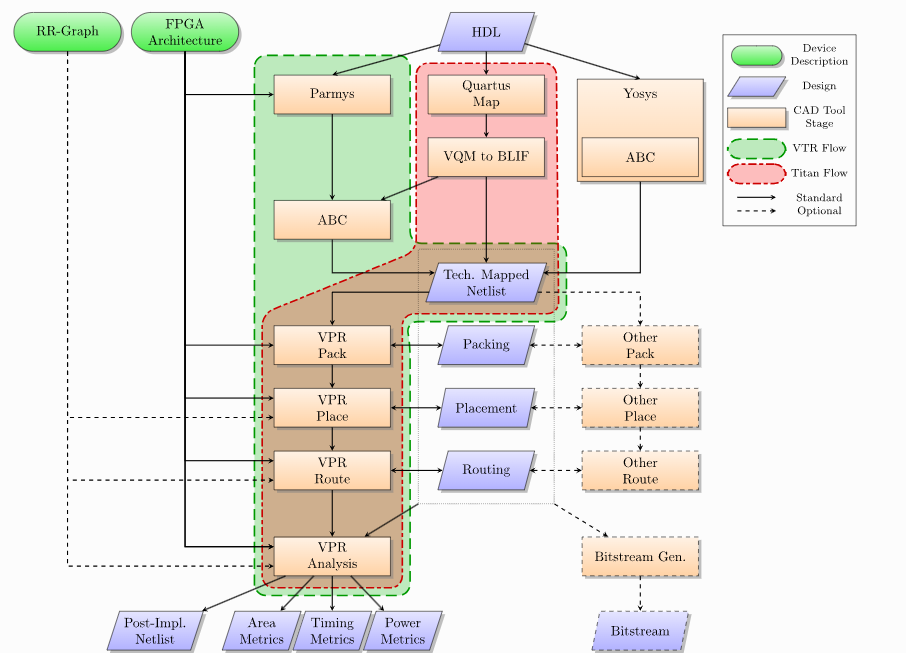
\includegraphics[scale = 0.8125]{Figures/vtr_cad_flow.png}}
	\caption{VTR CAD Flow\cite{vtr-toolchain-1}}
	\label{fig:vtr cad flow}
\end{figure}

The flow begins with Yosys, an open-source Verilog synthesis suite\cite{vtr-toolchain-2}. Yosys parses the Verilog HDL, performs initial optimizations, and generates a structural netlist in BLIF (Berkeley Logic Interchange Format), a textual format that represents gate-level designs. BLIF is widely used as a standard intermediate format in logic synthesis and academic CAD tools.

The generated BLIF netlist is then passed to ABC, a logic optimization and technology mapping tool developed at UC Berkeley\cite{vtr-toolchain-3}. ABC performs logic restructuring and maps logic functions onto basic gate primitives compatible with FPGA LUTs\cite{vtr-toolchain-4}. It also reduces logic depth and performs retiming optimizations where applicable. The output of ABC is a further optimized BLIF file used by VTR's core tools.

Next, the VPR (Versatile Place and Route) engine takes over. VPR performs three major tasks:
\begin{enumerate}
	\item \textbf{Packing:} Groups logic elements (e.g., LUTs, FFs) into logic clusters (CLBs or LABs) based on FPGA architecture constraints.
	\item \textbf{Placement:} Assigns packed logic clusters to specific physical locations in the FPGA grid.
	\item \textbf{Routing:} Connects placed logic blocks using the programmable interconnect and switch boxes, while adhering to the routing architecture defined in the FPGA model.
\end{enumerate}

VPR concludes with analysis, reporting timing, area (in MWTA), and power estimates. These results form the basis for comparative benchmarking of various architecture configurations\cite{vtr-toolchain-5}.

One of VTR’s most powerful features is its architecture description framework. Custom FPGA architectures are described using XML files that specify logic block structures, interconnect topologies, routing switch types, I/O standards, timing models, and cluster configurations. These XML descriptions are parsed and interpreted by VPR, enabling researchers to design and evaluate unconventional architectures—such as carry-chain-enhanced FPGAs, multi-CLB tiles, or DSP-rich fabrics—without modifying the underlying toolchain source code.

Overall, the VTR toolchain provides a complete, transparent, and configurable flow that is essential for academic research and architectural benchmarking. Its integration of synthesis, logic mapping, placement, and routing, combined with custom architecture support, makes it an indispensable framework for the exploration and evaluation of FPGA designs tailored for emerging compute workloads like machine learning.

%% END OF THE SECTION - VTR TOOLCHAIN %%

%% START OF THE SECTION - FUNDAMENTALS OF PRINCIPAL COMPONENT ANALYSIS
\section{Principal Component Analysis (PCA)}
\subsection{Introduction and Evaluation Metrics}
Principal Component Analysis (PCA) is a statistical method used to transform a set of correlated variables into a new set of uncorrelated variables known as principal components. These components are linear combinations of the original variables, arranged in order of decreasing variance. The primary goal of PCA is to identify the most significant patterns within the data while reducing its dimensionality, which is particularly useful in scenarios where data interpretation, visualization, and computational efficiency are essential. The essence of PCA lies in projecting high-dimensional data onto a new coordinate system where the dimensions are ranked based on their contribution to the dataset's overall variance\cite{pca-1}\cite{pca-2}.

PCA is an unsupervised learning technique widely used in machine learning, computer vision, and scientific computing. It is especially valuable in dealing with datasets where multicollinearity exists, meaning that features are highly correlated. By identifying a new set of orthogonal basis vectors, PCA effectively removes redundancy and ensures that each principal component captures distinct, non-overlapping information about the dataset\cite{pca-3}. This is particularly beneficial in applications such as image compression, where PCA enables a significant reduction in the number of pixels required to reconstruct an image while preserving its essential structure, and in finance, where it helps identify latent factors influencing asset prices.

Consider a multi-feature dataset comprising M records and N features. Then, the PCA algorithm begins by standardizing the dataset to ensure that each feature contributes equally to the analysis. This involves subtracting the mean of each feature and dividing by its standard deviation, thereby transforming the data into a zero-mean, unit-variance form. Next, the covariance matrix, an NxN symmetric matrix capturing the pairwise relationships between features, is computed. This matrix provides insight into how different features vary with respect to one another. Following this, the eigenvalues and eigenvectors of the covariance matrix are determined through eigenvalue decomposition or Singular Value Decomposition (SVD). The eigenvectors represent the principal components—orthogonal directions in feature space along which data exhibits maximum variance—while the corresponding eigenvalues indicate the amount of variance captured by each component. The eigenvalues are then sorted in descending order, and the top k eigenvectors (corresponding to the largest eigenvalues) are selected to form a reduced k-dimensional subspace. Finally, the original dataset is projected onto these principal components, yielding a transformed representation where the most significant variance is retained while reducing the overall dimensionality.

The algorithm for PCA is given below-
\begin{enumerate}
	\item \textbf{Input:} Input dataset D with M rows and N features
	\item Center the dataset : For every feature, subtract the mean of the feature from each point to center the dataset about the mean
	\( x_{i} \longleftarrow x_{i} - \frac{1}{N}\sum x_{k} \)
	\item Compute the covariance matrix of the scaled down dataset
	\( C = X^{T}X \), where \( X^{T} \) is the transpose of the input dataset and Xis the input dataset
	\item Perform Singular Value Decomposition (SVD) on the covariance matrix C to procure the eigenvalues and eigenvectors of the covariance matrix \( C = VD^{2}V^{T} \), where V is the matrix whose columns are the eigenvectors of the covariance matrix and D is the diagonal matrix whose elements are the square of the eigenvalues
	\item Multiplying X and V would result in the principal components, and the eigenvectors of the top k eigenvalues are selected as the principal components
	\item \textbf{Output: } Required Principal Components from the Input dataset
\end{enumerate}

Once the eigenvalues and their corresponding eigenvectors have been computed, the next crucial step in PCA is selecting the appropriate number of principal components, k, that will effectively reduce the dimensionality while preserving most of the data's variance. There are two widely used methods for determining k: the variance contribution ratio and the cumulative variance contribution ratio\cite{pca-4}.

The variance contribution ratio (VCR) is a measure of how much variance each principal component explains relative to the total variance in the data. Given that PCA aims to retain the most significant patterns in the dataset, components with higher variance contributions are more valuable. The variance contribution ratio for the \( i^{th} \) principal component is given by:

\begin{equation}
	\label{eq:equation_1}
	P_i = \frac{\lambda_i}{\sum_{k = 1}^N\lambda_k}
\end{equation}

where \( i \) is the eigenvalue associated with the \( i^{th} \) principal component, and \( \sum_{k = 1}^N\lambda_k \) is the sum of all eigenvalues, which is directly proportional to the total variance of the dataset. By sorting the eigenvalues in descending order, the first few principal components will have the highest variance contribution ratios. Typically, a threshold is set, and only the components with a variance contribution above this threshold are retained. For instance, if the first three components have variance contributions of 40\%, 30\%, and 15\%, a common heuristic might be to select the first two or three components since they contribute the most to the total variance.

Instead of analyzing individual variance contributions, the cumulative variance contribution ratio (CVCR) provides a more holistic criterion for choosing k. It sums the variance contributions of the top k principal components to ensure that a sufficient proportion of the total variance is preserved. The cumulative variance contribution ratio for the top k components is given by:

\begin{equation}
	\label{eq:equation_3}
	CP_i = \frac{\sum_{k = 1}^i \lambda_k}{\sum_{k = 1}^N \lambda_k}
\end{equation}

The goal is to select k such that $CVCR_{k}$ exceeds a predefined threshold, typically 95\% or 99\%. This ensures that the selected principal components retain most of the dataset's variance while reducing dimensionality.

For example, suppose the cumulative variance contribution for the first four principal components is 85\%, 92\%, 97\%, and 99\%. If an application requires at least 95\% variance retention, selecting the first three components would be sufficient.

In real-world scenarios, a scree plot (a plot of eigenvalues versus component index) is often used to visualize variance contributions. The "elbow point" of this plot, where eigenvalues begin to level off, serves as an intuitive indicator of an appropriate k. Alternatively, domain-specific constraints, computational efficiency considerations, and the trade-off between information preservation and dimensionality reduction influence the final choice of k.

\subsection{Case Study on Principal Component Analysis}
As an example, consider the wine dataset from the University of California-Irvine’s ML repository\cite{pca-5}. The Wine Recognition dataset from the UCI Machine Learning Repository is a classic classification dataset used to distinguish between three varieties of wine grown in the same region of Italy. Based on the results of chemical analysis, each sample represents a wine derived from one of the three cultivars. The dataset aims to evaluate how well different physicochemical characteristics can be used to identify the grape variety. The dataset comprises of the below feature set, as shown in Table.\ref{tab:summary of original features}.

\begin{table}[h]
	\centering
	\fontsize{10}{12}\selectfont
	\caption{Summary-Original Features}
	\label{summary of original features}
	\begin{tabular}{|p{3cm}|c|c|l|}
		\hline
		\textbf{S.No} & \textbf{Feature Index} & \textbf{Feature}\\
		\hline
		%\hline
		1 & F1 & Alcohol\\
		\hline
		2 & F2 & Malic Acid\\
		\hline
		3 & F3 & Ash\\
		\hline
		4 & F4 & Alcalinity of Ash\\
		\hline
		5 & F5 & Magnesium\\
		\hline
		6 & F6 & Total Phenols\\
		\hline
		7 & F7 & Flavanoids\\
		\hline
		8 & F8 & Non flavanoid phenols\\
		\hline
		9 & F9 & Proanthocyanins\\
		\hline
		10 & F10 & Color Intensity\\
		\hline
		11 & F11 & Hue\\
		\hline
		12 & F12 & OD280 / OD315 for diluted wines\\
		\hline
		13 & F13 & Proline\\
		\hline
	\end{tabular}
	
	\label{tab:summary of original features}
\end{table}

Then, the covariance matrix of the dataset, providing an overview on the inter dependencies between the different features in the dataset, is shown in the Figure \ref{the covariance matrix}
% Covariance Matrix Image
\begin{figure}[H]
	\centerline{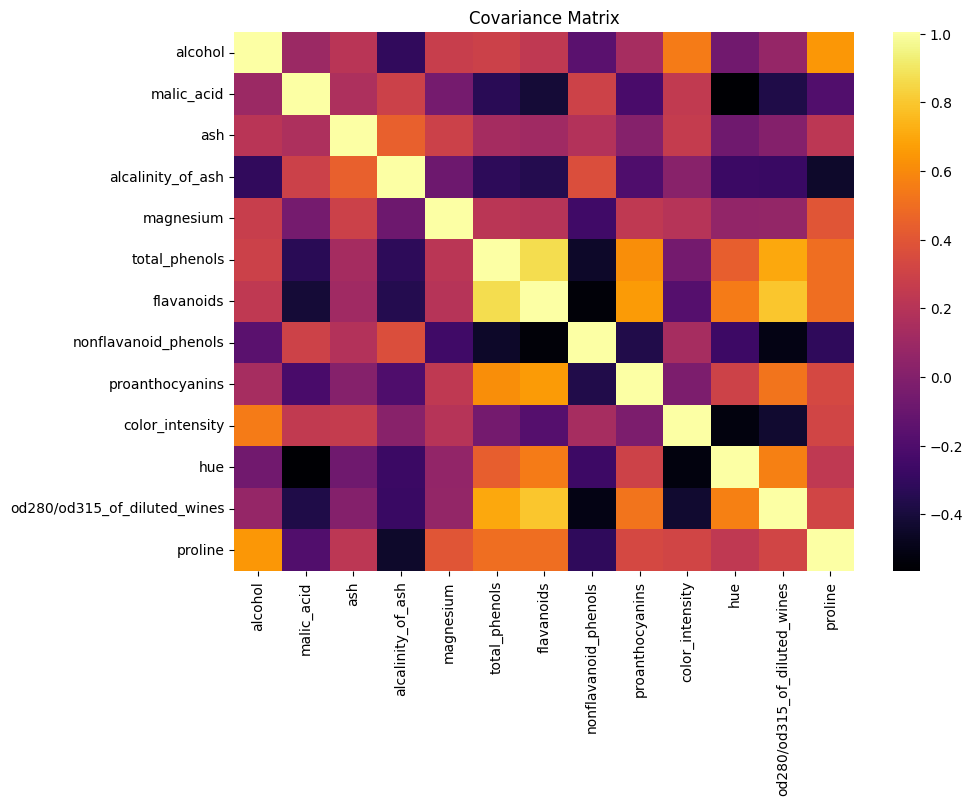
\includegraphics[scale = 0.8125]{Figures/covariance_matrix.png}}
	\caption{Covariance Matrix}
	\label{the covariance matrix}
\end{figure}

Further, the covariance matrix is decomposed into its eigenvalues and eigenvectors using Singular Value Decomposition, and the EVCR and CVCR across all the eigenvalues are calculated after arranging them in the descending order of their magnitude. Analysis of the variance contribution and cumulative variance contribution plots yield that the first 6 principal components would suffice and explain 80\% of the variance of the dataset.

The eigenvalues of the covariance matrix are computed and displayed in Table \ref{tab:eigenvalues of covariance matrix}. The eigenvectors corresponding to the top \textit{k} eigenvalues are obtained. The choice of \textit{k} will depend on the plot of explained variance ratio v/s the number of principal components chosen as shown in Figure \ref{pca ratio plot}

\begin{table}[h]
	\centering
	\fontsize{10}{12}\selectfont
	\caption{Eigenvalues of Covariance Matrix}
	\label{tab:eigenvalues of covariance matrix}
	\begin{tabular}{|p{3cm}|c|}
		\hline
		\textbf{PC\textsubscript{i}} & \textbf{Eigenvalue} \\
		\hline
		%\hline
		PC1 & 4.706\\
		\hline
		PC2 & 2.497\\
		\hline
		PC3 & 1.446\\
		\hline
		PC4 & 0.919\\
		\hline
		PC5 & 0.853\\
		\hline
		PC6 & 0.642\\
		\hline
		PC7 & 0.551\\
		\hline
		PC8 & 0.348\\
		\hline
		PC9 & 0.289\\
		\hline
		PC10 & 0.251\\
		\hline
		PC11 & 0.226\\
		\hline
		PC12 & 0.169\\
		\hline
		PC13 & 0.103\\
		\hline
	\end{tabular}
	
	\label{table:3}
\end{table}

The variance contribution ratio and the cumulative variance contribution ratio are calculated and displayed in Table \ref{variance contribution ratio of the principal components}. The line in Figure \ref{pca ratio plot} represents the principal component variance contribution ratio v/s the number of principal components chosen while the bars highlight the cumulative variance contribution ratio v/s the number of components chosen. It is seen that both the plots tend to saturate at higher principal components. Thus, it can be concluded that the first few principal components explain the majority of the data-set while the contribution of variance explained by the higher principal components is very less.

\begin{table}[h]
	\centering
	\fontsize{10}{12}\selectfont
	\caption{Variance and cumulative ratios}
	\label{table:4}
	\label{variance contribution ratio of the principal components}
	\begin{tabular}{|p{3cm}|c|c|}
		\hline
		\textbf{PC\textsubscript{i}} & \textbf{P\textsubscript{i}} & \textbf{CP\textsubscript{i}} \\
		\hline
		%\hline
		PC1 & 0.362 & 0.362\\
		\hline
		PC2 & 0.192 & 0.554\\
		\hline
		PC3 & 0.111 & 0.665\\
		\hline
		PC4 & 0.071 & 0.736\\
		\hline
		PC5 & 0.066 & 0.802\\
		\hline
		PC6 & 0.049 & 0.851\\
		\hline
		PC7 & 0.042 & 0.893\\
		\hline
		PC8 & 0.027 & 0.920\\
		\hline
		PC9 & 0.022 & 0.942\\
		\hline
		PC10 & 0.020 & 0.962\\
		\hline
		PC11 & 0.017 & 0.979\\
		\hline
		PC12 & 0.013 & 0.992\\
		\hline
		PC13 & 0.008 & 1\\
		\hline
	\end{tabular}
\end{table}

% INSERT VARIANCE CONTRIBUTION PLOTS FIGURE HERE
\begin{figure}[H]
	\centerline{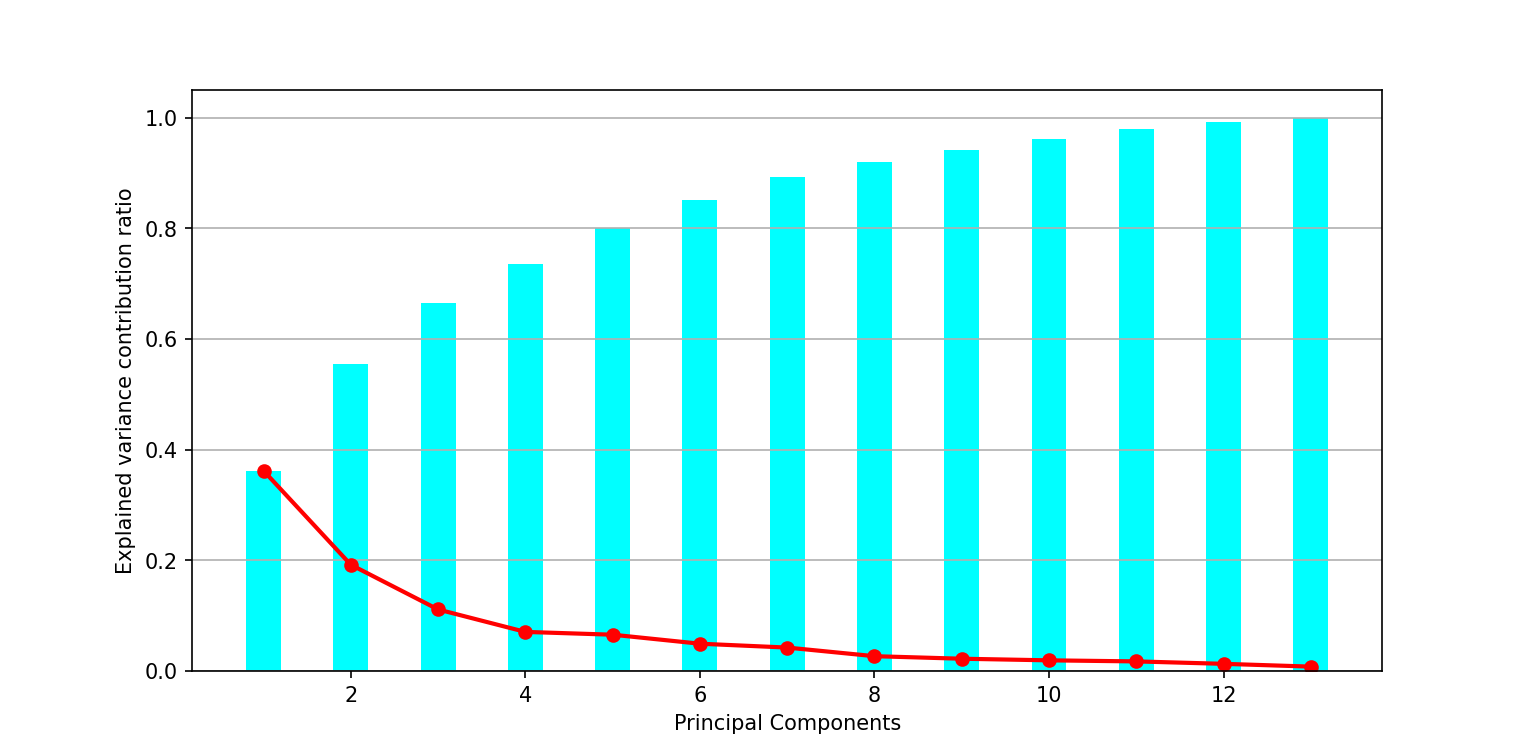
\includegraphics[scale = 0.75]{Figures/variance graph 2.png}}
	\caption{PCA Ratio Plot}
	\label{pca ratio plot}
\end{figure}

As 80\% of the variance can be captured from the first 5 principal components, the processed dataset with the first 5 principal components can be displayed in Table \ref{table:3}.

\begin{table}[h]
	\centering
	\caption{PCA Processed Table : First 5 records}
	\begin{tabular}{|p{3cm}|c|c|c|c|c|}
		\hline
		\fontsize{10}{12}\selectfont
		\textbf{S.No} & \textbf{PC1} & \textbf{PC2} & \textbf{PC3} & \textbf{PC4} & \textbf{PC5}\\
		\hline
		%\hline
		1 & 3.316751 & -1.443463 & -0.165739 & -0.215631 & 0.693043\\
		\hline
		2 & 2.209465 & 0.333393 & -2.026457 & -0.291358 & -0.257665\\
		\hline
		3 & 2.516740 & -1.031151 & 0.982819 & 0.724902 & -0.251033\\
		\hline
		4 & 3.757066 & -2.756372 & -0.176192 & 0.567983 & -0.311842\\
		\hline
		5 & 1.008908 & -0.869831 & 2.026688 & -0.409766 & 0.298458\\
		\hline
	\end{tabular}
	
	\label{table:5}
\end{table}


%% END OF THE SECTION - FUNDAMENTALS OF PRINCIPAL COMPONENT ANALYSIS %%


\begin{comment}
This chapter should discuss about the prerequisite learnings before the execution of the project. Organise and elaborate the theory and necessary fundamentals required for the execution of the project. You can use \verb|\subsections| and \verb|subsubsections| in this chapter.
\section{Contents of this chapter}
If a specific programming language is required for the project, a section can be allotted in this chapter to discuss it. 
\section{Contents of this chapter}
Tools used could be another possible section to discuss about the software tools used in the work. 
\section{Contents of this chapter}
The details in this chapter can be added in consultation with the project guide. For an internship based projects, subsections can be modified accordingly. 
\end{comment}

%% START OF THE SECTION - MATRIX MULTIPLICATION TECHNIQUES ON HARDWARE %%

\section{Matrix Multiplication Techniques on Hardware}
Matrix multiplication represents one of the most computationally intensive operations in linear algebra, imposing significant challenges for hardware implementations due to its high arithmetic complexity and substantial memory bandwidth requirements. The conventional matrix multiplication algorithm for two matrices exhibits a computational complexity of, necessitating multiply-accumulate (MAC) operations. On general-purpose processors, optimization strategies such as parallelization, cache tiling, and vectorized instructions are employed to enhance performance\cite{mm-technique-1}. However, as matrix dimensions increase, memory access patterns become a critical bottleneck, leading to inefficient execution on both central processing units (CPUs) and graphics processing units (GPUs), where frequent memory transactions constrain performance\cite{svd_architecture-4}.

Several algorithmic techniques have been proposed to mitigate the computational burden of matrix multiplication, including recursive methods such as Strassen’s algorithm and the Coppersmith-Winograd algorithm. Strassen’s method reduces computational complexity from to approximately by recursively decomposing matrices into smaller subproblems using a divide-and-conquer approach\cite{mm-techniques-2}. The Coppersmith-Winograd algorithm\cite{mm-techniques-3} further refines the complexity to . However, despite their theoretical efficiency, these recursive methods introduce significant overhead due to increased memory access, intricate indexing schemes, and complex branching operations, making them suboptimal for hardware acceleration, particularly on field-programmable gate arrays (FPGAs) and application-specific integrated circuits (ASICs). These architectures favor structured and highly parallel execution patterns that reduce control flow complexity and enhance data locality.

A widely adopted approach in hardware implementations is the use of systolic arrays, which offer a structured and highly efficient paradigm for matrix multiplication\cite{mm-techniques-4}. A systolic array, as shown in Fig.\ref{fig:systolic-array} consists of a regular arrangement of processing elements (PEs) that propagate data rhythmically in a synchronized manner, significantly reducing memory access overhead by maintaining intermediate results within local registers. The primary advantage of systolic arrays lies in their symmetry and spatial locality, facilitating predictable data flow and minimizing the necessity for intricate control logic and external memory transactions. Each PE executes a simple MAC operation and transfers partial results to adjacent units, thereby enabling high-throughput and low-latency computation. Due to their efficiency, systolic arrays have been extensively deployed in specialized hardware accelerators, including Google’s first-generation Tensor Processing Unit (TPU), which employed a matrix multiplication unit to expedite deep learning workloads\cite{mm-techniques-5}. The inherent parallelism and structured data movement of systolic arrays render them highly suitable for hardware-accelerated principal component analysis (PCA), where large-scale matrix operations, such as covariance matrix computation and eigendecomposition, demand computational efficiency. By leveraging systolic arrays, hardware accelerators achieve substantial performance improvements over CPU- and GPU-based approaches, thereby enabling real-time and large-scale PCA computations in machine learning, computer vision, and scientific computing applications.

\begin{figure}
	\centerline{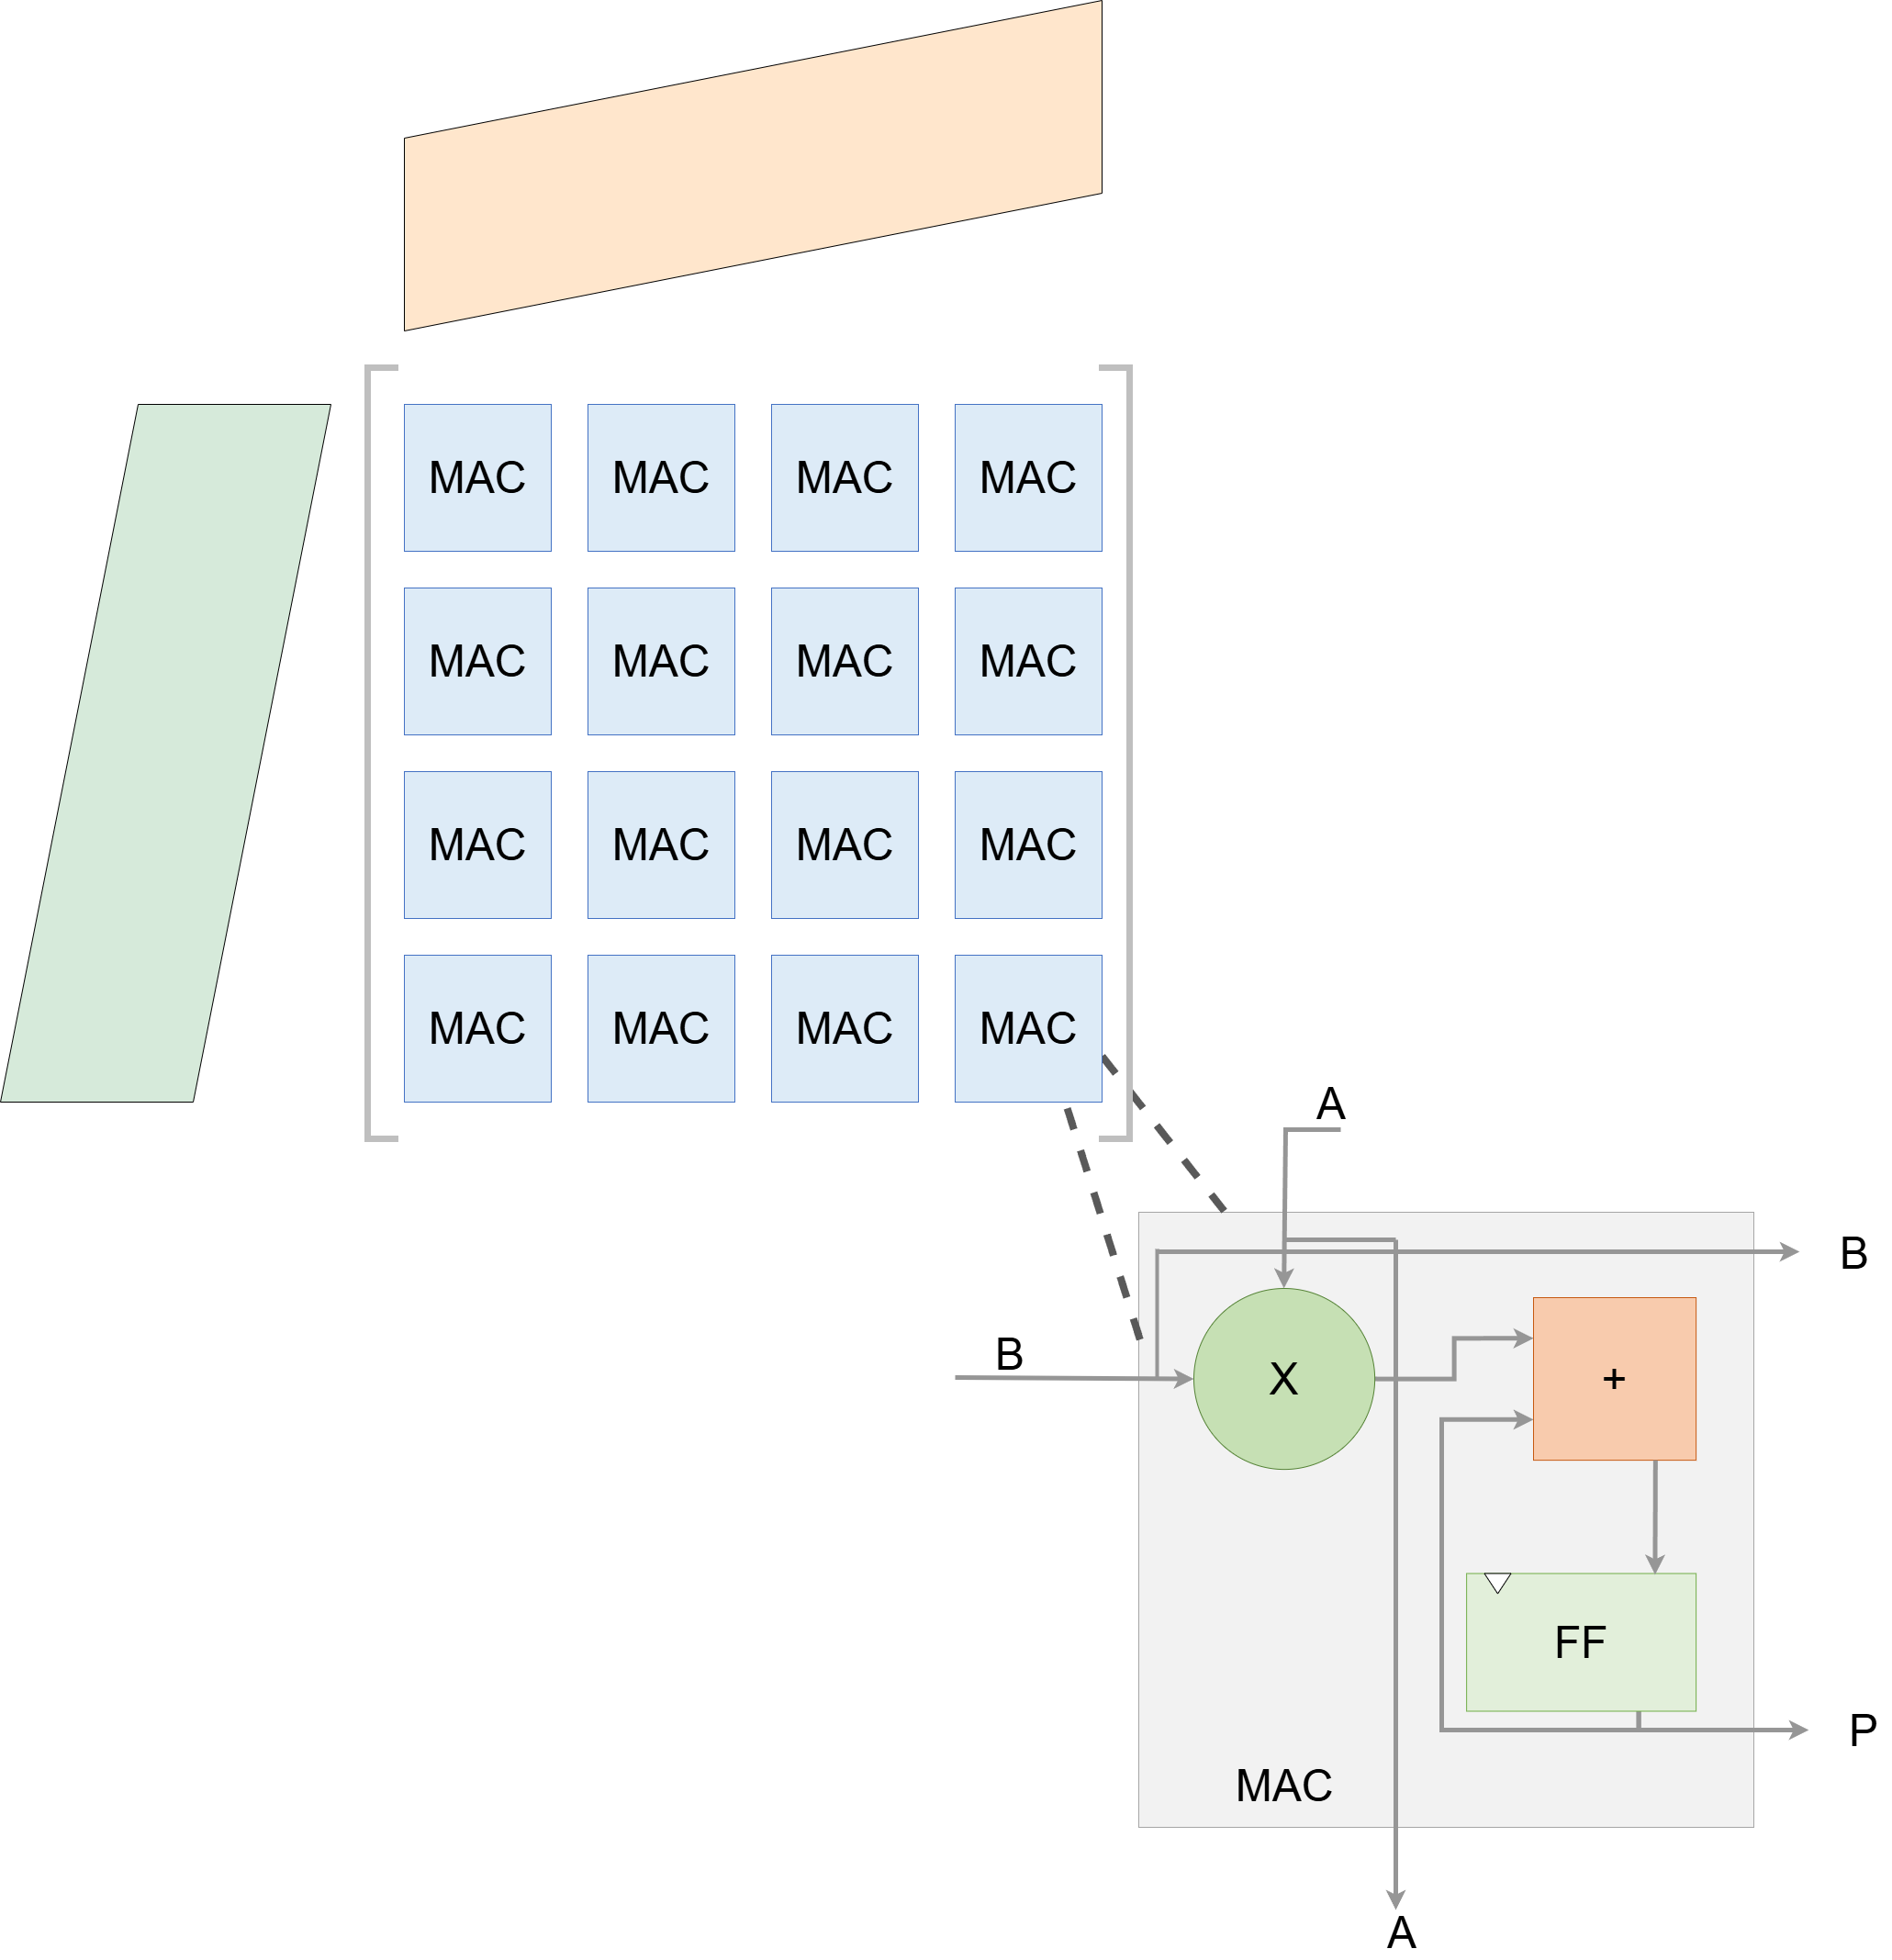
\includegraphics[scale = 0.15]{Figures/systolic_array_v2.png}}
	\caption{Systolic Array Architecture}
	\label{fig:systolic-array}
\end{figure}



%% END OF THE SECTION - MATRIX MULTIPLICATION TECHNIQUES ON HARDWARE %%

%% START OF THE SECTION - SINGULAR VALUE DECOMPOSITION ON HARDWARE %%
\section{Singular Value Decomposition on Hardware}
Singular value decomposition (SVD) is a fundamental operation in numerous scientific and engineering domains; however, its computational complexity poses substantial challenges, particularly for large-scale matrices. Two prominent approaches for computing SVD are the Jacobi algorithm and the Golub-Kahan algorithm, each possessing distinct computational characteristics and implications for hardware acceleration. The Jacobi algorithm, in both its one-sided and two-sided variants, iteratively applies Givens rotations to nullify off-diagonal elements, progressively transforming the matrix into diagonal form\cite{svd_architecture-6}. Singular values emerge along the diagonal, while the corresponding singular vectors are accumulated via successive orthogonal transformations. A notable advantage of the Jacobi method is its intrinsic parallelism, allowing Givens rotations to be applied independently to different matrix elements, thereby facilitating efficient concurrent execution. This parallel structure renders the Jacobi algorithm particularly well-suited for hardware acceleration on FPGAs, GPUs, and custom ASICs, where parallel computing resources can be fully utilized to expedite convergence.

Conversely, the Golub-Kahan algorithm employs a fundamentally different strategy by first reducing the matrix to a bidiagonal form via Householder reflections, followed by iterative QR decomposition to compute singular values\cite{svd-hardware-1}. An example of the Golub-Kahan algorithm was implemented in \cite{svd-hardware-2}, where the SVD was accelerated in Orthogonal Frequency Division Multiplexing (OFDM) for Multiple Signal Classification. This two-stage process introduces sequential dependencies that constrain parallelization. While the bidiagonalization phase ensures numerical stability, it involves substantial memory movement and matrix-vector multiplications, which present a bottleneck in hardware implementations. Furthermore, the QR iteration phase operates on the entire bidiagonal structure rather than individual matrix elements, leading to increased computational complexity and limited parallel execution capabilities. These inherent constraints make the Golub-Kahan algorithm less attractive for hardware implementations where efficiency and parallelism are paramount.

A key advantage of the Jacobi algorithm over Golub-Kahan is its superior numerical stability, particularly in handling ill-conditioned matrices. In numerical computations, ill-conditioned matrices exhibit small singular values that are highly sensitive to perturbations. The Jacobi method, leveraging iterative orthogonal transformations, ensures high precision in singular value computation while minimizing the accumulation of rounding errors. Each Givens rotation operates on a localized subset of matrix elements, thereby maintaining numerical accuracy throughout the transformation process. Conversely, the Golub-Kahan algorithm, particularly during its QR iteration phase, is susceptible to numerical instability due to repeated matrix factorizations, which amplify rounding errors over successive iterations. Consequently, the Jacobi approach is preferable for applications requiring high-precision singular value computations, including signal processing, control systems, and machine learning\cite{svd-hardware-3}.

From a hardware implementation perspective, the Jacobi algorithm aligns well with systolic array architectures, which are commonly employed for accelerating linear algebra computations. The ability to apply Givens rotations in parallel across multiple off-diagonal elements facilitates the design of highly efficient systolic arrays, where each processing unit performs localized transformations while maintaining communication with neighboring units. This distributed computation model significantly enhances throughput and reduces latency relative to sequential methodologies\cite{svd-hardware-4}. In contrast, the Golub-Kahan algorithm’s reliance on sequential bidiagonalization and QR factorization impedes efficient mapping onto systolic architectures, making it less desirable for FPGA and ASIC implementations.

Furthermore, the Jacobi algorithm’s reliance on element-wise transformations, rather than explicit matrix multiplications, leads to lower memory bandwidth requirements—a critical advantage in hardware accelerator design. Memory bandwidth often constitutes a limiting factor in high-performance computing applications, and minimizing data movement is essential for achieving energy efficiency and high-speed execution. The Golub-Kahan method, in contrast, involves multiple matrix-vector multiplications during the bidiagonalization process, exacerbating memory access demands and reducing suitability for low-power, high-efficiency hardware architectures.

Given these advantages, the Jacobi algorithm emerges as the preferred choice for hardware-accelerated SVD computation, particularly in FPGA- and ASIC-based systems. Its high parallelizability, superior numerical stability, efficient memory utilization, and compatibility with systolic architectures render it an optimal candidate for large-scale matrix computations in domains such as machine learning, image processing, and scientific computing. While the Golub-Kahan algorithm remains a robust option for general-purpose CPU-based implementations, its sequential constraints and elevated memory demands render it suboptimal for dedicated hardware acceleration scenarios.

\subsection{Jacobi Eigenvalue Decomposition}
The goal of PCA is to compute the eigenvalues and eigenvectors of the covariance matrix of a dataset. The Jacobi algorithm accomplishes this by iteratively applying orthogonal transformations to diagonalize the matrix.

The Jacobian Eigenvalue algorithm is presented below-
\begin{enumerate}
	\item \textbf{Input:} A symmetric covariance matrix \( C \) of dimension \( N \) x \( N \)
	\item Initialise the Eigenvector matrix \( V \) = \( I \). This matrix would accumulate the rotations
	\item Identify indices \( p \) and \( q \) such that  \( |c_{pq}| \) is the largest off diagonal element. The element would be reduced to zero in subsequent rotations
	\item Compute the rotation angle \( \theta \), that would zero out \( c_{pq} \). This is given by the equation \( 2\theta = \frac{2c_{pq}}{c_{pp} - c_{qq}} \)
	\item Calculate the value of \( cos(\theta) \) and \( sin(\theta) \)
	\item Construct an identity matrix \( R_{pq} \), and modify it such that \( R_{pp} = cos(\theta) \), \( R_{pq} = sin(\theta) \), \( R_{qp} = -sin(\theta) \), \( R_{qq} = cos(\theta) \)
	\item Apply the rotation as described by the equation \( C^{'} = R^{T}_{pq}CR_{pq} \)
	\item Update the Eigenvector Matrix \( V = VR \)
	\item The algorithm converges when all the off diagonal elements of \( C \) are below a specified tolerance \( \epsilon \)
	\item Columns of \( V \) are Eigenvectors
	\item \textbf{Output:} Return the Eigenvalue Decomposition of \( C \).
\end{enumerate}

Hence The Jacobian algorithm is the prefferred choice for hardware accelerator SVD computation. Particulary in FPGA and ASIC board systems\cite{svd-hardware-5}. Its highly parallelizable in nature superior numerical stability, efficient memory usage, and compatibility with systolic array architectures make it an ideal candidate for large - scale matrix computations in applications such as machine learning, image processing and scientific computing. 

%% END OF THE SECTION - SINGULAR VALUE DECOMPOSITION ON HARDWARE %%

%% START OF THE SECTION - INTRODUCTION TO CORDICs %%
\section{Introduction to CORDICs}
The Coordinate Rotation Digital Computer (CORDIC) algorithm is a highly efficient iterative method used for computing a variety of mathematical functions, including trigonometric, hyperbolic, logarithmic, and exponential functions. Developed by Jack Volder in 1959\cite{cordic-3} and later extended by Walther, CORDIC is particularly well-suited for hardware implementations such as Field Programmable Gate Arrays (FPGAs) and Application-Specific Integrated Circuits (ASICs) due to its ability to perform computations using only shift-and-add operations, avoiding the need for costly multipliers. This makes CORDIC an essential building block in digital signal processing (DSP), computer graphics, and scientific computing applications where real-time performance and efficient hardware utilization are critical. The algorithm operates by performing a sequence of iterative micro-rotations to approximate the desired function, making it particularly useful in FPGA-based architectures where hardware efficiency and low power consumption are crucial\cite{cordic-1}.

The CORDIC algorithm is based on the principle of vector rotation in a Cartesian coordinate system. Given an initial vector \( (x_{0}, y_{0}) \), the goal is to rotate it by an angle \( \theta \) to obtain a new vector \( (x^{'}, y^{'}) \) without using multiplication operations. This is accomplished by performing a series of micro-rotations of fixed angles that converge to the desired rotation. The core mathematical equations governing CORDIC in rotation mode are:
% CORDIC Equation-1
\begin{equation}
	\label{eq:equation_3}
	x_{i+1} = x_{i} - y_{i}d_{i}2^{-1}
\end{equation}

% CORDIC Equation-2
\begin{equation}
	\label{eq:equation_3}
	y_{i+1} = y_{i} + x_{i}d_{i}2^{-1}
\end{equation}

% CORDIC Equation-3
\begin{equation}
	\label{eq:equation_3}
	z_{i+1} = z_{i} - d_{i}tan^{-1}(2^{-1})
\end{equation}

where \( x_{i} \) and \( y_{i} \) are the coordinates of the vector in iteration \( i \), \( z_{i} \) is the angle that is progressively reduced to zero, \( d_{i} \) is the direction, determined as \( d_{i} = sign(z_{i}) \) ensuring that the angle is reduced in magnitude at each step. Here, \( 2^{-i} \) represents the micro-rotation scaling factor and \( tan^{-1}(2^{-i}) \) represents the precomputed constant for each iteration.

The iterative nature of the CORDIC algorithm means that each step rotates the vector by a smaller angle, refining the approximation with each iteration. Since multiplication by \( 2^{-i} \) is equivalent to a right bitwise shift, the entire computation involves only additions and shifts, making it extremely hardware-friendly.

CORDIC is particularly well-suited for FPGA-based hardware acceleration due to its shift-and-add architecture. Many FPGA vendors, including Xilinx and Intel, provide optimized CORDIC IP cores that can be easily integrated into hardware designs\cite{cordic-2}. The implementation consists of a series of iterative processing units, each responsible for executing one iteration of the algorithm. These units are pipelined to improve throughput, allowing multiple computations to be performed simultaneously.

% Cordic rotation angle Image
\begin{figure}[H]
	\centerline{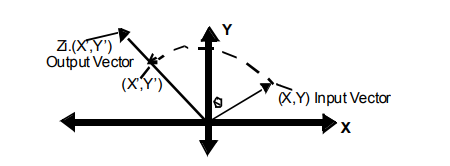
\includegraphics[scale = 0.80]{Figures/AMD_1.png}}
	\caption{CORDIC Rotation}
	\label{cordic rotation}
\end{figure}


%% END OF THE SECTION - INTRODUCTION TO CORDICs %%

%% START OF THE SECTION - CACHE ARCHITECTURE AND MODELING %%
\section{Cache Architecture and Modeling}
The performance of compute-bound and memory-bound applications, particularly in machine learning and signal processing accelerators, is significantly impacted by memory hierarchy efficiency. Cache design, including mapping strategies, write policies, and cache modeling techniques, plays a central role in improving data locality, reducing access latency, and optimizing energy use. This section explores foundational cache architectures, behavioral policies for write misses, real-world benchmarks used for cache modeling, and the use of CACTI for memory subsystem analysis.

\subsection{Direct Mapped Caches}
A direct-mapped cache, as shown in Fig.\ref{fig:direct-mapped-cache-arch}, represents the simplest form of address mapping in cache memory, where each block in main memory is mapped to exactly one location (or set) in the cache. Address decomposition in this cache type typically includes three fields: offset, index, and tag. The index field selects a unique cache line, and the tag is used to validate that the correct data is stored in that line. While this makes the design low-overhead and fast in lookup, it introduces potential issues with conflict misses, particularly if multiple memory addresses map to the same index\cite{cache-1}.

\begin{figure}
	\centerline{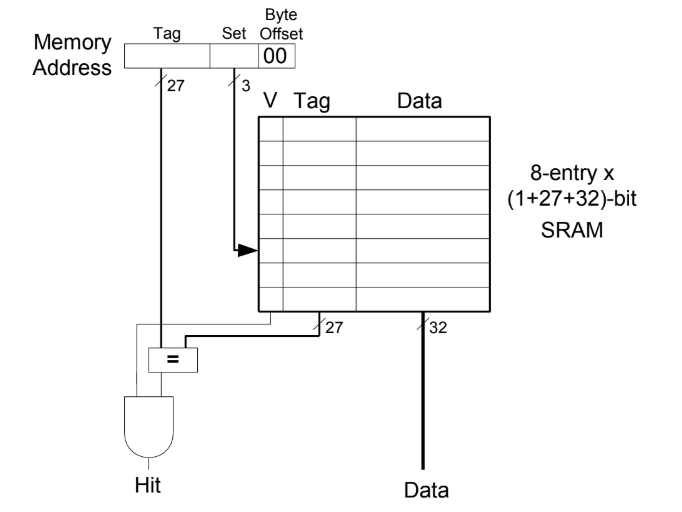
\includegraphics[scale = 0.6]{Figures/direct_mapped_cache_architecture.png}}
	\caption{Architecture of a Direct-Mapped Cache}
	\label{fig:direct-mapped-cache-arch}
\end{figure}

Despite their simplicity, direct-mapped caches can perform competitively when the access pattern exhibits high spatial locality and low contention. In FPGA-based accelerators, where deterministic timing is often more important than average-case throughput, direct-mapped caches offer predictable timing behavior and are easier to implement with minimal logic resources. However, for applications with large and irregular access footprints, such as matrix multiplication or sparse data reads, they may become a performance bottleneck due to frequent evictions.

\subsection{Cache Write Miss Policies}
\subsubsection{Write-Allocate Write-Miss Policy}
The write-allocate (also called fetch-on-write) policy dictates that when a write miss occurs, the block is first loaded from memory into the cache, and then the write is performed on the newly cached block. This policy assumes that the data being written is likely to be accessed again soon, benefiting from temporal locality. Write-allocate is usually combined with write-back, which reduces the number of memory write operations by deferring them until cache eviction.

In the context of FPGA accelerators for ML inference or training tasks, this policy is particularly useful when intermediate results — such as partial matrix products or activation values — are updated iteratively and accessed multiple times across computation cycles. By ensuring such values remain in the cache after being written, write-allocate reduces memory access latency and minimizes redundant memory transactions\cite{cache-3}.

Nonetheless, write-allocate incurs additional latency on write misses, as the cache line must first be fetched before the store can proceed. For latency-sensitive paths, this may create pipeline stalls or increase critical path pressure.

\subsubsection{Write-Around Write-Miss Policy}
In contrast, the write-around policy does not bring the missed data block into the cache. Instead, it bypasses the cache and writes directly to main memory. This is advantageous in workloads where written data is not expected to be reused, such as logging, streaming, or forward-only computations. By avoiding unnecessary cache fills, write-around reduces cache pollution, freeing up lines for data with higher reuse potential.

Write-around is often used alongside write-through caching, which ensures all writes update main memory immediately, preserving coherence across memory hierarchies. In FPGA accelerators like Manojavam, this policy is ideal for RHS matrix tiles in matrix multiplication, which are streamed in, used exactly once, and then discarded\cite{cache-3}.

However, write-around increases main memory bandwidth usage and may reduce energy efficiency if employed indiscriminately. It is best suited for write-once, read-never access patterns that dominate many preprocessing or forward-propagation stages in ML pipelines\cite{cache-4}.

\subsection{Cache Modeling Benchmarks}
Evaluating the effectiveness of cache policies requires realistic memory access patterns. Two well-established benchmark suites — LINPACK SAXPY and Livermore Loops — are used in this study to simulate cache behavior under practical conditions.

\subsubsection{LINPACK SAXPY Benchmark}
The SAXPY kernel (Single-Precision A·X Plus Y) is a Level-1 BLAS operation, represented by the equation:
\begin{equation}
	Y[i] = A.X[i] + B.Y[i]
\end{equation}

This pattern combines sequential reads from two input vectors with a write-back into one, making it ideal for testing read-write mixing, line reuse, and miss handling. In cache simulations, SAXPY reveals how well a system supports regular, linear memory access patterns with temporal locality\cite{cache-5}.

\subsubsection{Livermore Benchmark}
The Livermore Fortran Kernels (LFK) consist of 24 small programs, each designed to model a different class of scientific computation. These include operations like matrix multiplication, vector updates, numerical integration, and particle simulation. The Livermore benchmark of interest in this study, is given in the following equation-
\begin{equation}
	Z[i] = A.X[i] + B.Y[i]
\end{equation}

This equation involves multiple simultaneous memory reads, multiplication, and a final update, mimicking compute stages where multiple operands must be fetched concurrently. The reuse distance, line alignment, and miss rate behavior of this kernel provide deep insights into how the cache hierarchy responds to nested loops and indirect accesses.

Livermore Loops are especially useful for stress-testing multi-port caches, bank conflicts, and stride-sensitive performance — traits that become critical in loop-unrolled ML workloads\cite{cache-6}.

\subsection{CACTI Cache Modeler}
CACTI (Cache Access and Cycle Time Infrastructure) is a comprehensive tool for modeling cache and memory subsystems with respect to access latency, power consumption, and physical area. Originally developed by Hewlett-Packard Labs and later expanded by researchers at the University of Utah, CACTI has become a widely used framework for evaluating SRAM-based cache designs in both research and industrial contexts. It allows designers to explore how microarchitectural decisions — such as cache size, associativity, block size, number of ports, and banking — affect delay, energy, and silicon footprint\cite{cache-7}\cite{cache-8}.

At a high level, CACTI combines delay models for SRAM cells and peripheral logic with power and area estimators derived from accurate transistor-level characterizations. It simulates the read and write paths through the memory array, including precharge, sense amplification, wordline and bitline transitions, tag comparison, and output drivers. These computations are further refined by incorporating RC interconnect delay models for local and global wiring, providing timing estimates that closely reflect physical implementation constraints.

The tool accepts a range of parameters including total cache size, line size, associativity, number of banks and ports, and the target technology node. From this, it produces detailed reports on access latency, cycle time, dynamic and leakage power, and layout area. CACTI also supports different access modes — including sequential, fast, and normal — each modeling different levels of precharge and comparator overlap.

By enabling rapid design-space exploration across technology generations and architectural configurations, CACTI facilitates early-stage memory subsystem planning. It is particularly useful when evaluating trade-offs between latency, energy efficiency, and area — all of which are critical constraints in hardware accelerators, embedded processors, and SoC memory hierarchies. Its extensibility and compatibility with open-source flows make it an ideal modeling tool for cache-centric hardware research.

%% END OF THE SECTION - CACHE ARCHITECTURE AND MODELING %%

%% START OF THE SECTION - FPGA DESIGN FLOW %%
\section{FPGA Design Flow}
The FPGA design flow is a comprehensive process that transforms a high-level hardware description into a physical configuration bitstream, allowing the FPGA device to behave as the intended digital circuit. This multi-stage flow, as shown in Fig.\ref{fig:fpga-design-flow} is essential to ensure the design is functionally correct, meets timing requirements, and optimally utilizes hardware resources. Each stage builds upon the previous one, gradually refining the design until it is ready for deployment.

\begin{figure}[H]
	\centerline{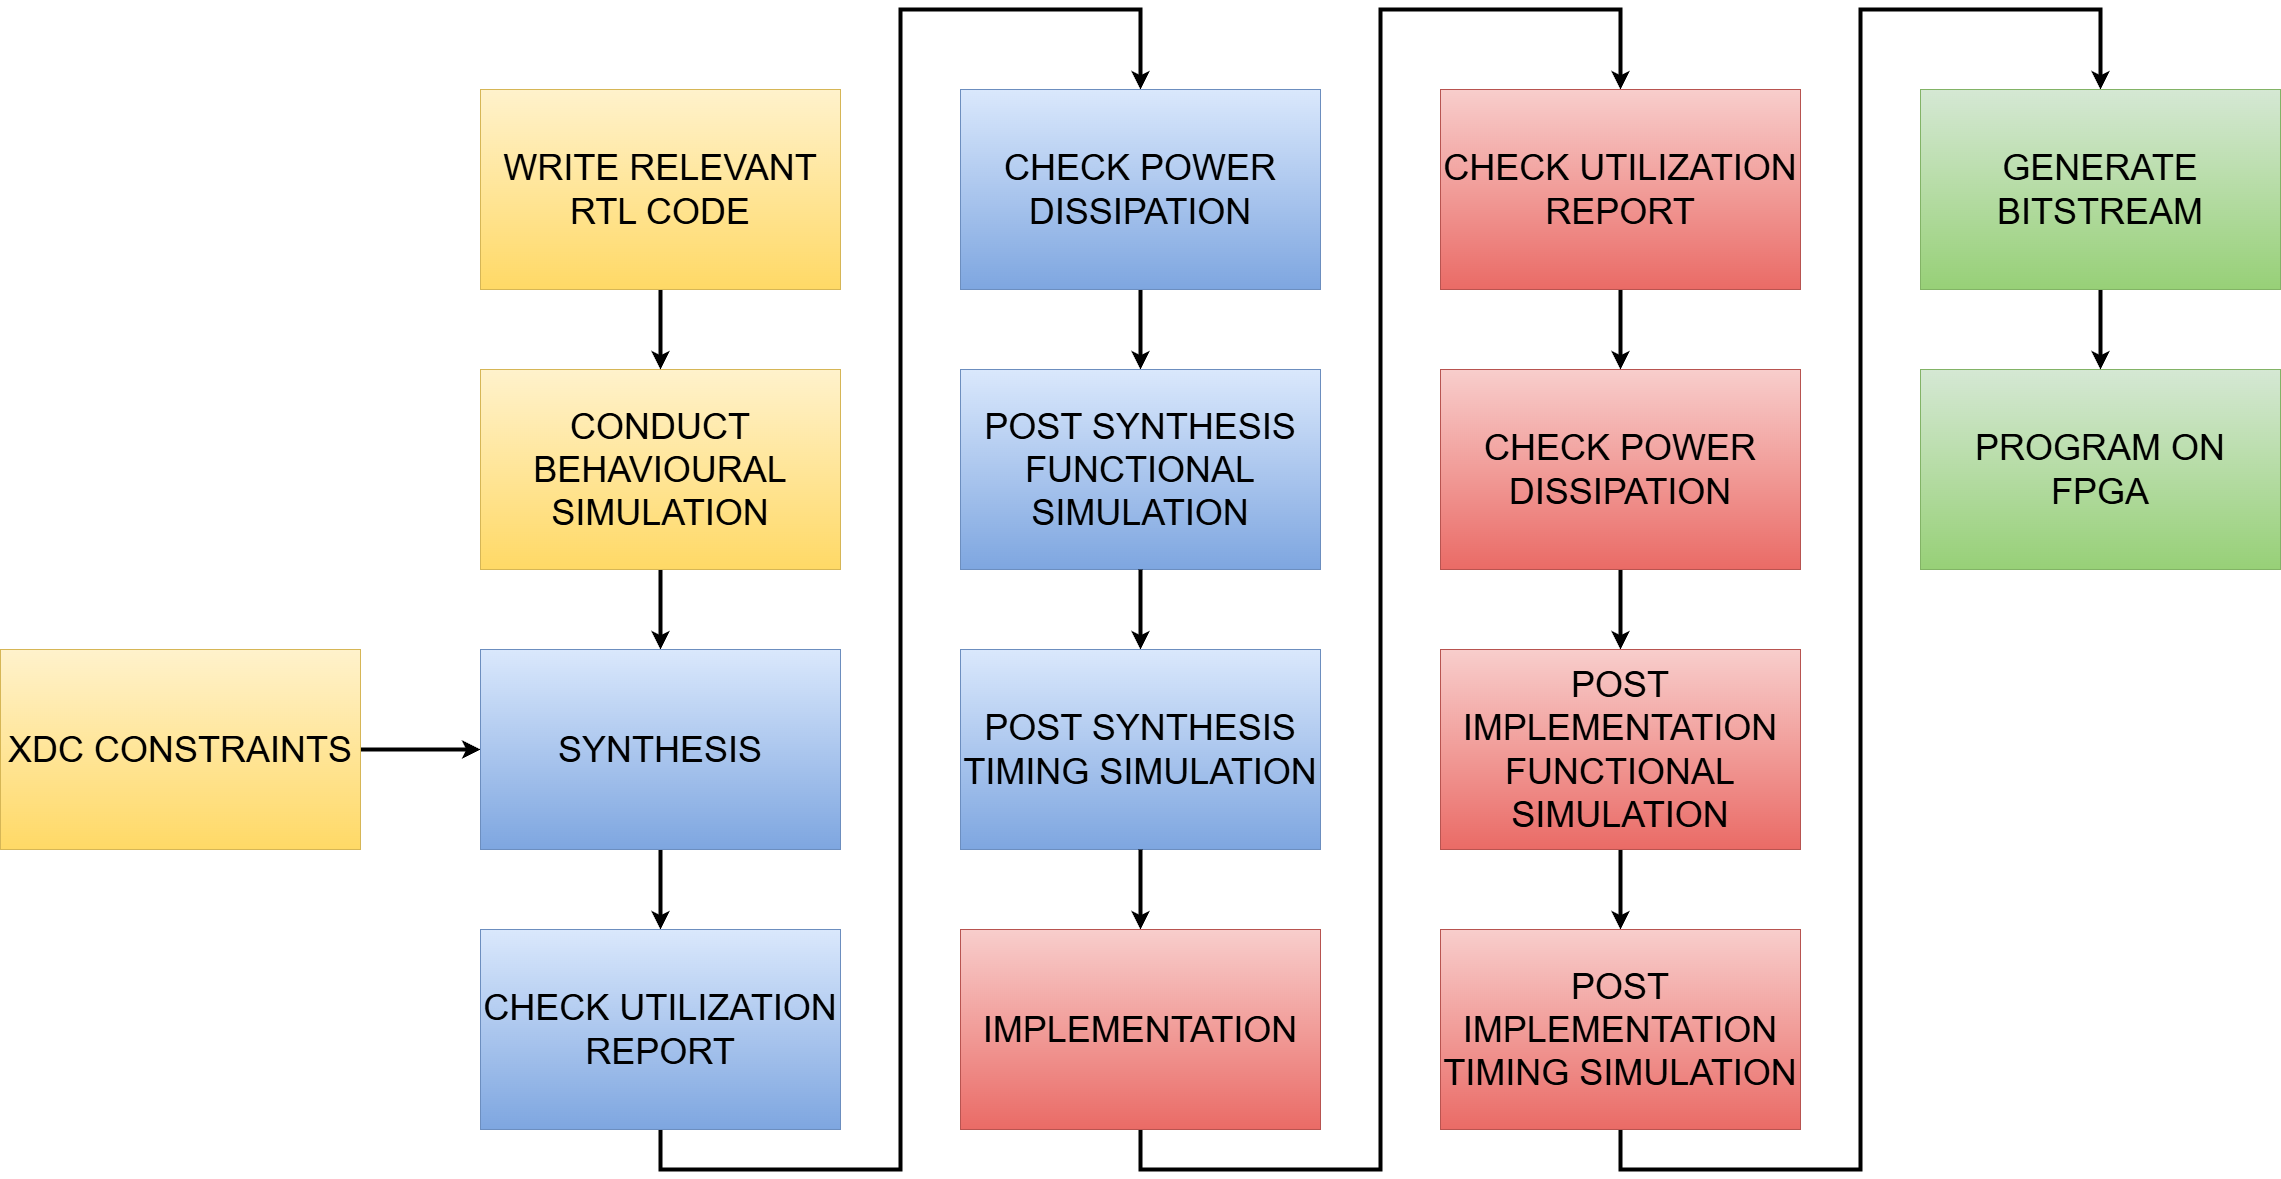
\includegraphics[scale = 0.2]{Figures/FPGA_design_flow_v2.png}}
	\caption{FPGA Design Flow}
	\label{fig:fpga-design-flow}
\end{figure}

\subsection{RTL Entry}
Register Transfer Level (RTL) entry represents the first and foundational step in the FPGA design process. Here, the digital system's behavior and structure are described using a hardware description language (HDL), most commonly Verilog or VHDL. The RTL abstraction focuses on the flow of data between registers and the operations performed on that data synchronized by clock signals.

Writing synthesizable RTL code requires deep understanding of digital logic design and coding guidelines to ensure that the code can be successfully transformed into hardware. Designers must focus on writing clean, modular, and reusable code with clear synchronous logic constructs, avoiding non-synthesizable constructs like delays or certain loops that can't be mapped to hardware. The RTL code typically includes the definition of combinational logic, synchronous state machines, arithmetic units, multiplexers, and register files.

This stage sets the design intent clearly and forms the basis for all subsequent synthesis and implementation steps. Good RTL design not only ensures functional correctness but also heavily influences the efficiency, speed, and area utilization of the final FPGA implementation.

\subsection{Behavioural Simulation}
Behavioral simulation is the process of verifying the RTL code at a functional level before any hardware synthesis or physical mapping. It is the first verification checkpoint, focused on confirming that the design logic behaves as expected under a wide range of input conditions without considering any timing delays.

In this phase, simulation testbenches are written to provide input stimuli and monitor outputs. Testbenches model realistic operating scenarios, edge cases, and corner conditions to verify the correctness of control paths, data paths, and overall system behavior. Common simulation environments include ModelSim, QuestaSim, and Vivado Simulator.

Behavioral simulation supports iterative debugging, allowing designers to detect and fix logic bugs early, thereby reducing the risk of expensive errors downstream. It also facilitates the validation of complex algorithms and state machine transitions before the design is locked for synthesis. This step is crucial to build confidence that the design will function correctly once synthesized and implemented.

\subsection{Synthesis}
Synthesis is a pivotal step where the RTL code is automatically translated into a gate-level representation compatible with the FPGA's architecture. This process converts abstract behavioral descriptions into an optimized network of logic gates, lookup tables (LUTs), flip-flops, multiplexers, and embedded blocks like DSP slices and block RAMs.

The synthesis tool, such as Xilinx Vivado or Synplify Pro, analyzes the RTL for logic equivalence, timing, and resource constraints, then performs optimizations including logic minimization, retiming, and resource sharing. The synthesis output is a Technology Mapped Netlist (TMNL) — a detailed description of the design using the primitives available in the target FPGA device.

The synthesis process also provides crucial reports indicating estimated resource utilization (LUTs, FFs, DSPs, BRAMs), maximum achievable clock frequency, and warnings or errors. Designers can tweak the RTL code or synthesis constraints to improve performance or reduce resource usage. A well-optimized synthesis directly influences the quality of results (QoR) of the overall design.

\subsection{Post Synthesis Simulation}
Once synthesis completes, post-synthesis simulation serves as the next verification stage to ensure that the synthesized netlist preserves the intended functionality of the RTL. Unlike behavioral simulation, this step uses the gate-level netlist and incorporates basic gate delays and timing models that reflect the synthesis tool’s understanding of the hardware implementation.

The simulation includes detailed signal propagation through logic gates and flip-flops, enabling detection of functional discrepancies introduced during synthesis optimization such as logic restructuring or resource sharing. Post-synthesis simulation helps verify that the design’s logical correctness remains intact and is crucial before committing to the implementation stage.

Additionally, this simulation helps designers spot issues related to glitches, race conditions, or unexpected logic behavior caused by gate-level transformations. It sets the foundation for accurate timing analysis and confirms that the design is ready for the more detailed physical implementation flow.

\subsection{Implementation}
Implementation is the stage where the synthesized netlist is physically mapped, placed, and routed onto the FPGA fabric. It consists of several intricate sub-steps that translate the logical design into a physical layout optimized for speed and resource utilization.
\begin{enumerate}
	\item \textbf{Translation:} Converts the synthesized netlist and constraints into a format suitable for implementation tools.
	\item \textbf{Mapping:} Assigns the synthesized logic elements like LUTs, flip-flops, DSP blocks, and BRAMs to the physical resources available on the FPGA device.
	\item \textbf{Placement:} Strategically determines the exact physical locations on the FPGA for each logic element, balancing the trade-offs between performance, congestion, and resource distribution. Placement algorithms aim to minimize critical path delays and interconnect complexity.
	\item \textbf{Routing:} Establishes physical connections between placed elements through the FPGA’s programmable routing fabric. Routing ensures that signals meet timing requirements and avoids routing congestion and cross-talk.
\end{enumerate}

This stage involves iterative optimization driven by timing constraints and resource availability specified in the constraints file. Modern FPGA tools use advanced heuristics and machine learning-based algorithms to find near-optimal placement and routing solutions.

Implementation generates detailed timing reports and resource utilization metrics. Achieving timing closure — meeting all timing constraints such as setup and hold times — is one of the most challenging aspects of the implementation phase.

\subsection{Post Implementation Simulation}
Post-implementation or timing simulation models the design’s behavior with full consideration of the detailed delays introduced by the actual physical placement and routing. This simulation uses the timing back-annotated netlist (SDF file) containing precise delay values for all interconnects and logic elements, reflecting the true operating conditions on the FPGA.

This stage verifies that the design meets timing constraints under worst-case delay scenarios and functions correctly with actual path delays, clock skews, jitter, and other physical effects. It helps identify timing violations, race conditions, and glitches that could lead to functional failures in silicon.

Post-implementation simulation is often the final functional verification step before generating the FPGA bitstream. Passing this simulation provides confidence that the design will operate reliably at the targeted clock frequency once programmed on the device.

\subsection{Xilinx Design Constraints}
The Xilinx Design Constraints (XDC) file is a vital input to synthesis and implementation tools, specifying the physical and timing requirements of the design. The XDC file uses the industry-standard Synopsys Design Constraints (SDC) syntax and allows precise control over various aspects of the FPGA implementation\cite{fpga-flow-1}.

Key components of an XDC file include:
\begin{enumerate}
	\item \textbf{Pin Assignments:} Mapping logical signals to specific FPGA I/O pins, ensuring correct electrical connections to external hardware interfaces such as sensors, memory modules, or communication lines.
	\item \textbf{Clock Definitions:} Specification of clock signals including frequency, duty cycle, waveform timing, and clock groups to guide timing analysis and optimization.
	\item \textbf{Timing Constraints:} Setup and hold time requirements, false path and multi-cycle path declarations, and exceptions that allow the tools to focus on critical timing paths.
	\item \textbf{Placement Constraints:} User directives for floorplanning, such as locking down specific logic blocks or I/O to fixed locations to optimize performance or meet design partitioning goals.
	\item \textbf{Physical Constraints:} Constraints related to voltage standards, slew rates, drive strengths, and other electrical characteristics. 
\end{enumerate}

Accurate and comprehensive constraints in the XDC file are essential for ensuring the design meets functional, timing, and interface specifications in the final FPGA implementation.

\subsection{Bitstream Generation}
Bitstream generation is the culminating step in the FPGA design flow, where the fully implemented design is converted into a binary configuration file that programs the FPGA device. This bitstream encodes all information regarding logic configurations, routing paths, clock setups, and I/O assignments, essentially ‘telling’ the FPGA how to physically realize the design.

The bitstream is generated by the FPGA vendor tools once timing closure is confirmed and the implementation results are satisfactory. The tool packages the design into a format compatible with the target FPGA device’s configuration memory, considering encryption, compression, and device-specific requirements.

After bitstream generation, the file is loaded onto the FPGA via programming interfaces such as JTAG, SPI, or Platform Cable USB. Once programmed, the FPGA starts operating as the designed digital system.

This final step is critical as any errors or timing violations detected after bitstream generation require returning to earlier design stages for correction. Successful bitstream generation signifies the completion of the FPGA design process and readiness for hardware testing and deployment.

%% END OF THE SECTION - FPGA DESIGN FLOW %%

%% START OF THE SECTION - ASIC DESIGN FLOW ON OPENLANE AND OPENRAM %%
\section{ASIC Design Flow on Openlane and OpenRAM}
ASIC design transforms RTL descriptions into manufacturable silicon layouts through a sequence of design stages. OpenLane, developed by the OpenROAD project\cite{asic-3}, is an open-source, fully automated ASIC backend flow that integrates various open-source EDA tools to streamline this process\cite{asic-1}. OpenRAM complements OpenLane by providing an open-source SRAM compiler, enabling automated generation of memory blocks essential for many ASIC designs\cite{asic-2}.

\subsection{Openlane Architecture and Flow}
OpenLane orchestrates the ASIC backend implementation starting from synthesized RTL and design constraints, producing a final verified layout. It integrates tools such as Yosys for synthesis, OpenDP for placement, TritonRoute for routing, and OpenSTA for timing analysis, all managed via Python scripts and containerized environments for reproducibility. The Openlane ASIC flow is depicted in Fig.\ref{fig:openlane-flow}.

\begin{figure}[H]
	\centerline{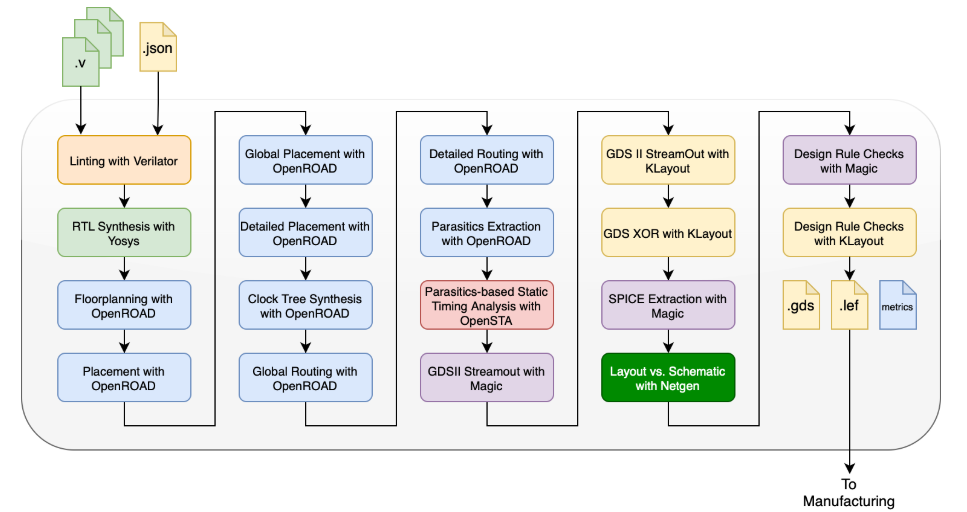
\includegraphics[scale = 0.75]{Figures/openlane_flow.png}}
	\caption{ASIC Openlane Flow\cite{asic-1}}
	\label{fig:openlane-flow}
\end{figure}

The key stages include-
\begin{enumerate}
	\item \textbf{Synthesis:} Converts RTL into a gate-level netlist optimized for the target technology.
	\item \textbf{Floorplanning:} Defines core area, I/O placement, and power grid setup.
	\item \textbf{Placement and Clock Tree Synthesis:} Assigns physical locations to cells and synthesizes the clock distribution network.
	\item \textbf{Routing:} Connects cells with metal layers while ensuring design rule compliance.
	\item \textbf{Verification:} Performs DRC, LVS, and static timing analysis.
	\item \textbf{GDSII Generation:} Creates the final layout file for fabrication.
\end{enumerate}

OpenLane uses YAML-based configuration files to customize design parameters such as technology libraries, floorplan dimensions, and clock frequencies, providing flexibility across different ASIC projects.

\subsection{OpenRAM Integration}
OpenRAM is a parameterizable, open-source SRAM compiler that automatically generates synthesizable RTL, physical layout, and timing models tailored to specified memory configurations like size, port count, and banking.

OpenRAM SRAM blocks integrate smoothly into the OpenLane flow by:
\begin{enumerate}
	\item Being instantiated directly in RTL or added post-synthesis as black-box macros.
	\item Undergoing placement and routing alongside standard cells during implementation.
	\item Providing accurate timing and power characterization models to assist timing closure and power estimation.
\end{enumerate}

This integration eliminates the need for manual SRAM design, accelerating ASIC development and improving design reliability.

%% END OF THE SECTION - ASIC DESIGN FLOW ON OPENLANE %%

\begin{comment}

\section{Use of Acronyms and Glossaries}
Acronyms are nothing but the short form of regular repeated word. Say for example, you have a repeat word "Integrated Circuits" and you want to use a short form for it as "IC". For which you have to first define the word and use it wherever you wanted to refer it.

First, let's look at the definition, which has to be entered in \texttt{Glossaries.tex} under \texttt{CoverPages} directory.
\begin{verbatim}
%\newacronym{<Ref>}{<Short-Form>}{<Expanded word>}
\newacronym{ic}{IC}{Integrated Circuits}
\end{verbatim}
In order to use the defined acronym, use the commands \verb|\gls{<Ref>}| as shown below

As an example, call the definition with \verb|\gls{ic}| and the outcome of it is reflected as, \gls{ic}.

Note: For the First time, the expanded form appears along with the Short-form definition inside parenthesis. But when the \verb|\gls{}| is repeated, only Short-form appears inside the parenthesis.

Now, let's look at the definition of symbols. Follow the syntax to define the symbol first, inside \texttt{Glossaries.tex} under \texttt{CoverPages} directory.
\begin{verbatim}
%\newglossaryentry{<Ref>}{name=<Symbol>, description={<description about the symbol>}, type=<List type>}
\newglossaryentry{rc}{name=$\tau$, description={Time constant}, type=symbolList}
\end{verbatim}

As an example, the rate of change is defined with \verb|\gls{rc}| and the outcome of it is reflected as, the rate of change is defined with \gls{rc}.

\vspace{0.75cm}

 \textbf{The chapters should not end with figures, instead bring the paragraph explaining about the figure at the end followed by a summary paragraph.}


After elaborating the various sections of the chapter (From Chapter 2 onwards), a summary paragraph should be written discussing the highlights of that particular chapter. This summary paragraph should not be numbered separately. This paragraph should connect the present chapter to the next chapter.
\end{comment}

This chapter outlined the essential theoretical and technical foundations supporting the two key aspects of the project: FPGA architectural exploration and the RTL-to-ASIC design of the Manojavam PCA accelerator. The FPGA section began by examining the internal structure of FPGAs, focusing on Configurable Logic Blocks (CLBs), lookup tables (LUTs), and routing elements such as switch boxes. It introduced the baseline Intel Stratix-10 architecture along with custom 4-bit Single and Double Carry Chain architectures optimized for low-precision arithmetic and parallel carry propagation. The importance of area, delay, and logic utilization as evaluation metrics was discussed in the context of machine learning hardware acceleration. The VTR toolchain was detailed, emphasizing the roles of Yosys (for Verilog synthesis), ABC (for logic optimization and technology mapping), and VPR (for packing, placement, routing, and analysis), along with the use of architecture description XML files for architectural specification.

The second part of the chapter focused on the Manojavam PCA accelerator, starting with matrix multiplication strategies that use 4×4 operand tiling and controller-driven tile streaming. It introduced systolic arrays based on TPU-style architectures and explained both weight-stationary and output-stationary dataflows to maximize throughput and regularity. The mathematical basis of PCA was discussed through covariance matrix formulation and the Jacobi method, highlighting the role of Givens rotations in eigendecomposition. Memory hierarchy design was explored through a block-streamed structure with private L1 and shared L2 caches, incorporating write-around and write-validate policies. The RTL design process was explained using Verilog and Vivado, covering simulation, synthesis, implementation, and power-timing analysis. The ASIC design flow was covered through OpenLane, detailing floorplanning, placement, routing, and GDSII generation, along with OpenRAM-based SRAM integration. Supporting tools such as CACTI and a custom simulator were used for cache modeling and compute latency analysis. Altogether, these foundations established the architectural, algorithmic, and tool-driven context necessary for the development and evaluation of the project's hardware systems.


%Chapter 3
\chapter{Design Methodology}

\begin{comment}
\indent\indent From Chapter 2 onwards, every chapter should start with an introduction paragraph. This paragraph should brief about the flow of the chapter. This introduction can be limited within 4 to 5 sentences. The chapter heading should be appropriately modified (a sample heading is shown for this chapter).But don't start the introduction paragraph in the chapters 2 to end with "This chapter deals with....". Instead you should bring in the highlights of the chapter in the introduction paragraph. 
\end{comment}

Designing efficient ML hardware requires a structured approach to both architectural modeling and accelerator development. This chapter outlines the methodology adopted for evaluating custom FPGA architectures using the VTR toolchain, with a focus on carry chain-based logic for arithmetic-heavy ML benchmarks. In parallel, it details the step-by-step design of the Manojavam PCA accelerator, including its systolic matrix engine, cache hierarchy, and controller structure. Key design decisions, supporting models, experimental workflows, and analytical formulations are also discussed, setting the foundation for implementation and result analysis in the subsequent chapters.

\section{Specifications of FPGA Architectural Exploration}
The motivation behind this architectural exploration stems from the need to understand how the internal composition of FPGA logic blocks — particularly the nature of carry propagation and the use (or absence) of hardened arithmetic units — influences the efficiency of mapping arithmetic-heavy workloads. In the context of machine learning (ML) applications, such as matrix multiplications, digital filters, and accumulation pipelines, the performance of the underlying hardware is highly sensitive to how well the architecture supports fast and compact arithmetic operations. While modern commercial FPGAs like Intel Stratix-10 or Xilinx Versal feature hardened DSP blocks to optimize multiply-accumulate operations, many research-grade or open-source FPGA fabrics, as well as ASIC-grade RTL flows, rely instead on carry chains composed of basic logic elements. Studying the tradeoffs between heterogeneous architectures (with DSP hard blocks) and homogeneous logic-only designs (with serial or parallel carry chains) offers insights into how arithmetic-dense applications behave across a broader architectural spectrum.

To facilitate this analysis, three target architectures were employed in the study, each described in the VTR architectural XML format. The first is a Stratix-10-like architecture, modeling hardened multipliers and adder trees to resemble a modern high-performance heterogeneous FPGA. The second is a homogeneous architecture featuring a 4-bit single carry chain, where carry propagation is strictly serial across four 1-bit full adders, emulating delay-intensive arithmetic behavior. The third is a 4-bit double carry chain architecture that introduces parallel carry propagation paths, allowing partial carries to resolve concurrently, thus improving throughput for wider additions. These three configurations allow us to explore the performance spectrum from hardened, low-latency arithmetic to logic-only, delay-sensitive arithmetic styles.

All three architectures were evaluated under a fixed routing and interconnect model — specifically, a standard island-style routing architecture as defined in VTR. Each architecture maintains the same routing switch box style, wire segmentation, and global resource availability. The only changes lie in the logic block definitions — namely, the composition of BLEs (basic logic elements), the presence or absence of carry chains, and how multipliers are realized (hardened vs. synthesized). This isolation of variables ensures that performance differences are directly attributable to logic architecture rather than routing artifacts or placement constraints.

To assess the practical implications of these architectural differences, a fixed set of HDL benchmarks were synthesized and mapped onto each architecture. These benchmarks consist of:
\begin{enumerate}
	\item \textbf{Adder Trees:} 2-level and 3-level summation trees for fixed-point operands, stressing chained addition performance.
	\item \textbf{FIR Filters:} Pipelined and unpipelined FIR structures with and without hard multipliers. For carry-based architectures, multipliers were implemented using Wallace-tree style adder networks, exercising the carry chain fabric intensively.
\end{enumerate}

Performance was quantified using three key metrics:
\begin{enumerate}
	\item \textbf{Operational Frequency (f)} — defined as the reciprocal of the longest delay path:
	\item \textbf{Critical Path Delay (D)} — the maximum timing delay (in nanoseconds) from any input to output in the post-place-and-route design.
	\item \textbf{Area (MWTA)}  — a weighted logic utilization model inspired by VTR
\end{enumerate}

This setup provides a controlled environment to understand how different logic architectures influence the performance of ML-relevant workloads, enabling data-driven decisions for future FPGA or domain-specific accelerator designs.

\section{FPGA Architectural Modeling in VTR}
To perform a rigorous architectural exploration, three FPGA fabric configurations were modeled using the Verilog-to-Routing (VTR) toolchain: (1) Intel Stratix-10-like heterogeneous FPGA with hardened DSP blocks, (2) a homogeneous FPGA with a 4-bit carry chain within each logic block (single chain), and (3) a variant with two parallel 4-bit carry chains (double chain). These configurations were described using VTR’s XML-based architecture specification language, with a focus on modeling complex logic blocks (CLBs), interconnects, and hard blocks like multipliers and memories.

\subsection{CLB Architecture and Carry Chain Design}
At the heart of each fabric lies its CLB (Configurable Logic Block) design. In the Stratix-10 model, the CLB closely mimics Intel’s Adaptive Logic Module (ALM), which includes 6-input fracturable LUTs and dedicated hardened carry logic. The carry chains here are tightly coupled with the LUT outputs, and propagate between logic elements using explicitly defined \textbf{direct} connections — one for incoming carry from the previous LAB and another for chaining between elements within a CLB. The structure supports efficient arithmetic mapping and pipelining in DSP-like workloads

The 4-bit single chain architecture departs from this by implementing a simplified carry chain that connects five logic elements linearly within a single chain per CLB. The XML model defines a chain pattern from \textbf{fle1[0].cout} to \textbf{fle1[1].cin}, and so on, terminating at \textbf{fle1[4]}. The carry-in for this chain originates from an external \textbf{cin} pin on the CLB, and the carry-out from the last element is routed to \textbf{cout}. This mimics the operation of older generation FPGAs or minimalist logic fabrics where a single chain is adequate for low-to-medium complexity arithmetic.

The double chain architecture enhances this further by including two parallel 4-bit chains, allowing for simultaneous arithmetic operations across two independent data paths. This is evident from how two sets of fle instances are used \textbf{(fle[0:4] and fle[5:9])}, each having its own \textbf{cin} and \textbf{cout} wiring paths. The interconnect model explicitly defines chaining within each set as well as the routing from the LAB to the CLB inputs and outputs, capturing parallelism in low-precision arithmetic mapping.

\subsection{Routing and Interconnects}
All three architectures share a uniform island-style routing structure characterized by segmented wires, programmable switch boxes, and connection blocks. The routing tracks are uniformly distributed across the horizontal (x) and vertical (y) directions with a peak utilization factor of 1.0. Wilton-style switch blocks were used \textbf{(fs=3)} to enable flexible connectivity and short detours around congested regions, and \textbf{ipin-cblock} switches were employed for linking routing wires to logic block inputs. This standardization ensures that any differences in performance metrics can be attributed primarily to the internal CLB and carry chain design rather than the routing infrastructure.

\subsection{Hardblocks and Memory Modeling}
Across all architectures, the multiplier logic is defined using a \textbf{pb-type} block for a 27×27-bit fracturable multiplier. Internally, this multiplier can operate in multiple modes: two 18×19-bit multipliers or one 27×27-bit unit, reflecting the flexibility of real-world DSP blocks. These modes enable trade-offs between precision and resource utilization. The internal delay characteristics are also modeled, with a delay of approximately 1.825 ns for each 18×19 multiplier, aligning with data from Intel Arria-10 chips fabricated in 22nm technology nodes.

Memory blocks, though not heavily emphasized in this study, are modeled as simple RAM blocks with fixed delays. These provide compatibility with workloads such as FIR filters and adder trees that may require coefficient or state storage.

In essence, this section formalizes the modeling of three FPGA architectural variants in VTR, emphasizing differences in CLB composition and carry chain capabilities. While the routing, memory, and multiplier subsystems were kept largely consistent, the varying styles of arithmetic support within the logic blocks allowed us to examine their influence on performance and area when mapped with arithmetic-heavy benchmarks. These architecture files served as the foundation for place-and-route trials, allowing us to extract meaningful comparisons across design metrics such as critical path delay, logic utilization, and peak operating frequency.

\section{Methodology for FPGA Architectural Exploration using VTR}
To evaluate how different FPGA architectures handle machine learning-oriented workloads, the Verilog-to-Routing (VTR) toolchain was employed as the core design exploration framework. This methodology aimed to systematically analyze architectural features—particularly carry chains and DSP-based blocks—and their effect on logic utilization, timing, and packing behavior across a series of ML-inspired benchmarks. The complete flow begins with Verilog-based HDL descriptions of the benchmark circuits, followed by synthesis, logic optimization, physical design using VPR, and ends with extraction and comparative analysis of key performance metrics.

The input to the flow consists of Verilog modules representing arithmetic-dominated circuits such as adder trees and FIR filters. These were either directly synthesized using ODIN-II, which is integrated into the VTR toolchain, or preprocessed using Yosys when finer control over synthesis was required—particularly in cases where multiplication operators were explicitly replaced with adder networks to force logic mapping onto carry chains. This preprocessing helped standardize the structure of the circuits, ensuring that architecture-dependent variations observed in later stages were genuine and not synthesis artifacts.

Post synthesis, the resulting intermediate logic network is passed through ABC, a logic optimization and technology mapping tool that is tightly integrated with VTR. ABC performs a series of transformations to simplify and balance the logic, minimize delay, and prepare the design for physical mapping. The output of this step is a BLIF (Berkeley Logic Interchange Format) file, which represents the optimized netlist and becomes the primary input to the placement and routing stages of the flow.

The next phase of the methodology involves running the BLIF file through the Versatile Place and Route (VPR) engine. VPR operates on a user-defined FPGA architecture specified via XML, which details the structure and interconnect of the logic blocks, switch boxes, routing channels, carry chains, and DSP blocks. In this project, three architecture files were used to model: (1) a baseline Intel Stratix-10–style architecture with hardened DSP blocks, (2) a 4-bit single carry chain architecture where each CLB is equipped with a single serial carry propagation path, and (3) a 4-bit double carry chain architecture that provides enhanced arithmetic throughput through dual carry paths.

The VPR engine performs packing, placement, and routing tailored to the architecture file. The packing stage clusters logic elements into configurable logic blocks (CLBs). For carry chain-based architectures, packing favors tight clustering of adders to exploit localized carry propagation paths, while in DSP-based designs, packing tends to consolidate multiplier-heavy logic into fixed-function DSP blocks. This difference leads to significant architectural trade-offs: carry chain-based designs often offer higher utilization efficiency and better support for low-precision arithmetic, whereas DSP-based architectures perform better for large-width multipliers but may suffer from resource underutilization. After packing, VPR places the clusters on the grid and performs routing to connect them, finally conducting timing analysis to evaluate path delays, clock frequency potential, and signal integrity.

At the conclusion of each run, VPR produces detailed reports that include critical path delay, logic block usage, routing channel widths, switch utilization, and cluster packing efficiency. These metrics serve as the basis for evaluating architectural performance. For example, in adder-dense benchmarks, the carry chain architectures often showed improvements in delay and area metrics due to efficient local routing and minimal use of global interconnects. In contrast, the Stratix-10–style DSP architecture displayed strengths in FIR filters with wide datapaths, though at the cost of higher power and underutilized multiplier blocks for narrower bit-widths.

Given the extensive number of architecture-benchmark combinations, the entire VTR flow was automated using shell scripts, allowing batch execution of synthesis, placement, routing, and report extraction across all benchmark-architecture pairs. This not only reduced manual intervention but also ensured consistency across evaluations, enabling a scalable and repeatable testing framework. In addition to this, a separate Python-based preprocessing pipeline was developed to transform Verilog benchmark designs. Specifically, FIR filter designs that originally used the multiplication \textbf{(*)} operator were programmatically converted into structurally described Wallace tree multipliers, facilitating accurate mapping to carry chain logic and enabling architecture-aware synthesis. This Python module acted as a custom Verilog code generator, automatically restructuring arithmetic-heavy blocks to reflect fine-grained logic suitable for low-bit-width architectures. These preprocessed designs, when passed through the VTR flow, provided insights into how architectural choices affect resource utilization and timing when optimized arithmetic representations are employed.

\section{FPGA Analysis Metrics Equations}
In order to quantitatively evaluate and compare the performance of different FPGA architectures for ML-relevant workloads, three primary metrics were employed in this study: Operational Frequency, Critical Path Delay, and Area in MWTA (Minimum Width Transistor Area). These metrics are derived from the post-routing reports generated by the VTR toolchain and offer insights into the timing performance and spatial efficiency of each architecture.

\subsection{Operational Frequency}
Operational frequency indicates the maximum clock rate at which the synthesized design can be reliably executed on the given FPGA architecture. It is the inverse of the critical path delay and is computed as:
\begin{equation}
	f_{op} = \frac{1}{T_{cp}}
	\label{eq:operational_Frequency_vtr}
\end{equation}

Where $T_{cp}$ is the critical path delay (in seconds), reported by VPR.

To express $f_{op}$ in MHz, the equation becomes:
\begin{equation}
	f_{op}(MHz) = \frac{10^{3}}{T_{cp}(ns)}
	\label{eq:operational_Frequency_vtr_mhz}
\end{equation}

Where the symbols retain their usual meaning.

\subsection{Critical Path Delay}
The critical path delay refers to the longest path delay through the combinational logic of the design, which determines the minimum possible clock period. This metric reflects the delay bottleneck of the circuit and is a direct output of the VPR timing analysis engine.

\begin{equation}
	T_{cp} = max(\sum_{i}d_{i})
\end{equation}

Where $d_{i}$ is the delay of each logic element and interconnect on a specific path. 

\subsection{Area in MWTA Units}
Area is measured in terms of Minimum Width Transistor Area (MWTA), a normalized metric used by VTR to estimate the silicon area occupied by the design on a theoretical FPGA fabric. MWTA is a technology-independent metric that allows fair comparison across architectures.

The Area in MWTA units is described in the equation below:
\begin{equation}
	A_{MWTA} = \sum_{i}(Area_{block_i}) + \sum_{j}(Area_{routing_j})
\end{equation}

Where $Area_{block_i}$ includes the area of logic blocks, flip-flops, and DSPs, and $Area_{routing_j}$ includes switch boxes, connection boxes, and wire segments.

This metric provides a coarse estimation of the physical footprint and is particularly useful in evaluating the area efficiency of logic structures such as carry chains versus DSP blocks.

Together, these metrics provide a comprehensive basis for analyzing architectural performance. While operational frequency and critical path delay capture timing behavior, the MWTA area metric enables hardware designers to assess the compactness and logic density achieved under each architecture configuration.

\section{Architecture of the Manojavam Accelerator}
The Manojavam PCA accelerator is a fully RTL-based hardware architecture designed to compute Principal Component Analysis in a power-efficient and scalable manner. PCA is a core operation in machine learning pipelines and involves two principal computational steps: covariance matrix computation and eigendecomposition via the Jacobi method. Manojavam is organized into three tightly coupled stages: the Covariance Matrix Computation Unit, the Jacobian Unit, and the Rotation Unit. Together, these components operate on streamed matrix tiles, allowing the accelerator to process large datasets efficiently. A defining characteristic of Manojavam is the reuse of datapaths between the covariance and rotation stages, enabling the architecture to optimize for both area and performance without duplicating compute logic. The complete design is implemented in Verilog HDL, simulated in Vivado, and validated through both FPGA and ASIC (OpenLane) flows. The high level architecture of Manojavam is as shown in Fig.\ref{fig:manojavam high level architecture}.

\begin{figure}
	\centerline{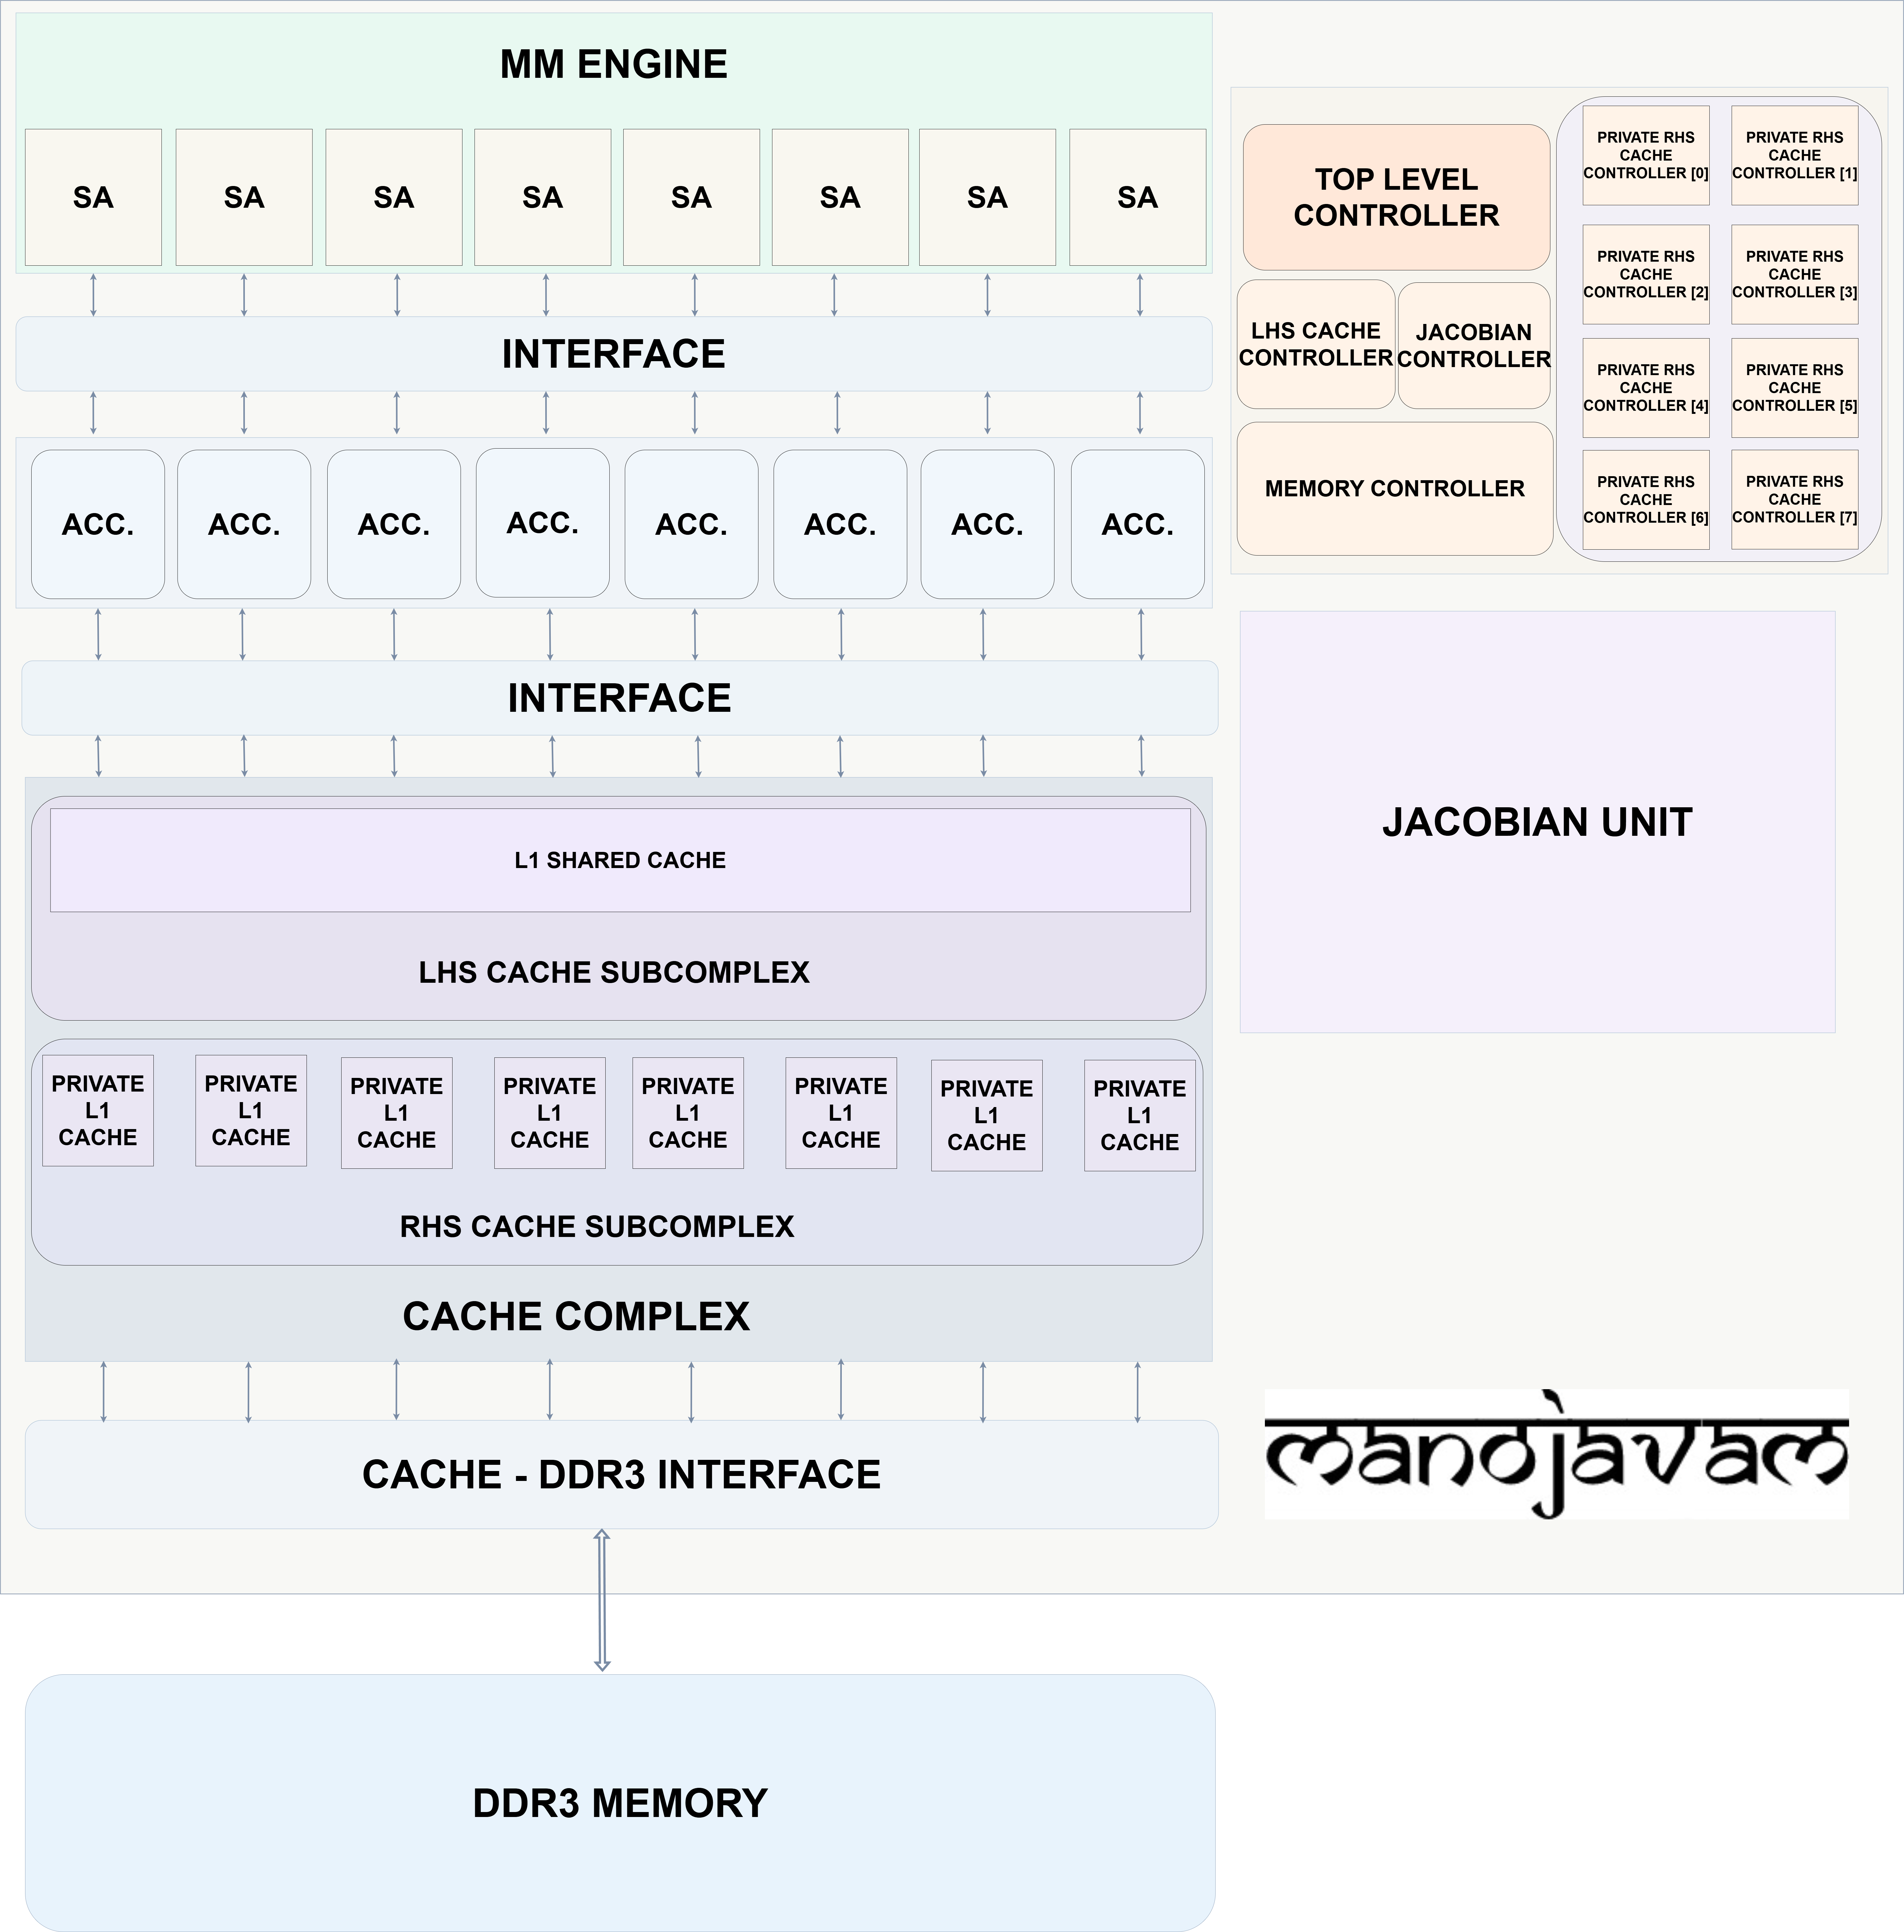
\includegraphics[scale = 0.05]{Figures/manojavam_architecture_v4.png}}
	\caption{High Level Architecture of Manojavam}
	\label{fig:manojavam high level architecture}
\end{figure}

\section{Matrix Multiplication Engine}
The Covariance Matrix Computation Unit is tasked with constructing the symmetric matrix $C = X^{T}X$ where $X$ is the input dataset matrix with mean-subtracted and standardized values. In PCA, this matrix encodes the pairwise correlations between input features and forms the foundation for identifying dominant eigenvectors. Due to the high dimensionality and streaming nature of ML datasets, direct computation of $X^{T}X$ is memory- and compute-intensive. Manojavam addresses this challenge using a tiled matrix multiplication approach, where the input matrix $X$ is divided into a series of smaller 4×4 operand tiles, allowing submatrix-level parallel processing and spatial data reuse.

These tiles are streamed into a Matrix Multiplication Engine (MM Engine) comprising eight independent 4×4 systolic arrays, each designed to operate in parallel on a different tile pair. Systolic arrays are chosen for their regular structure and pipelined data movement, which reduces control complexity and maximizes throughput. Each array follows a weight-stationary dataflow model, where one operand (typically $X^{T}$) is held stationary within the array registers, while the second operand (typically $X$) flows through the pipeline. This model enables each multiply-accumulate (MAC) unit to reuse its stored operand multiple times, significantly reducing memory bandwidth requirements and off-chip traffic\cite{chap3-2}.

Large-scale matrix multiplication poses a fundamental bottleneck in hardware accelerators due to limited on-chip memory and compute parallelism. Manojavam addresses this challenge through block streaming matrix multiplication, shown in Fig.\ref{fig:tiled-MM}. It is a technique that decomposes large input matrices into smaller, fixed-size tiles — typically matching the size of the systolic array (e.g., 4×4 blocks). These tiles are streamed sequentially through a systolic compute fabric, allowing partial products to be accumulated incrementally across time without requiring the full matrix to reside on-chip. This tiling approach drastically reduces memory bandwidth pressure and allows effective reuse of operands stored in local buffers\cite{chap3-1}. Moreover, by orchestrating tile loading and compute through a staged controller and cache hierarchy, Manojavam overlaps data transfer with computation, ensuring that the processing elements remain fully utilized. This technique enables the accelerator to scale to arbitrarily large matrices within the limited BRAM resources of the FPGA, thereby making high-dimensional covariance computations and PCA viable even under strict hardware constraints.

\begin{figure}
	\centerline{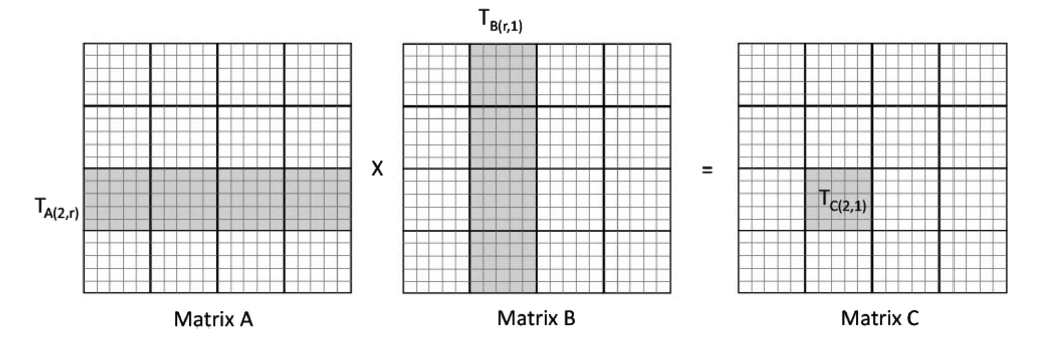
\includegraphics[scale = 0.75]{Figures/tiled_MM.png}}
	\caption{Illustration of Tiled Matrix Multiplication}
	\label{fig:tiled-MM}
\end{figure}

The systolic arrays process operand tile pairs in a wavefront pattern, where rows of $X^{T}$
and columns of $X$ are sequentially injected into the array, and intermediate products are propagated and summed through the grid of MAC units. The output of each array is a 4×4 partial product matrix corresponding to a block of the full covariance matrix. These partial products are not stored directly; instead, they are routed to a corresponding matrix accumulator, which collects and accumulates the results across multiple tile passes. Each accumulator is mapped one-to-one with a systolic array and implements a register or BRAM-based accumulation buffer, capable of holding intermediate values until all contributing tile products for that block have been processed.

Operand tiles are delivered to each systolic array through a structured input stream managed by Matrix Padding Units. These units take flattened 1D representations of the matrix stored in memory and reshape them into 2D tile structures, ensuring that operands are correctly aligned for the systolic pipeline. This is depicted in Fig.\ref{fig:systolic_array_setup}. Additionally, the padding units handle zero-padding for tiles at the matrix boundary when the input dimensions are not multiples of 4. This abstraction simplifies control logic and guarantees correctness across arbitrary input sizes.

\begin{figure}
	\centerline{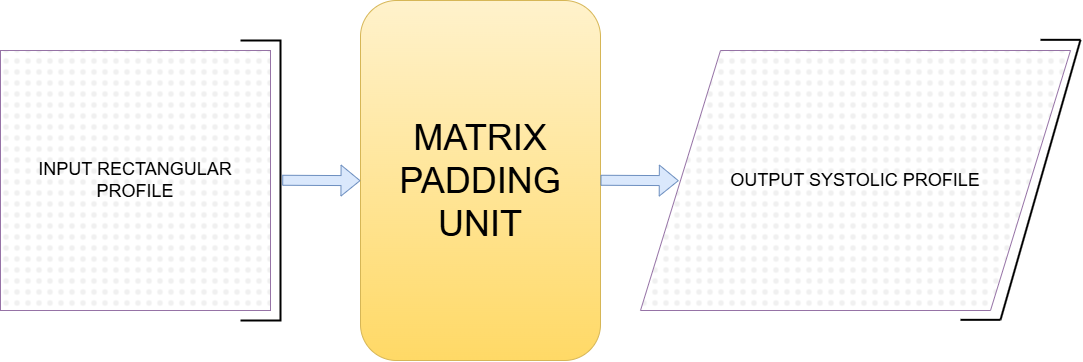
\includegraphics[scale = 0.35]{Figures/systolic_array_setup.png}}
	\caption{Systolic Operand Setup by Matrix Padding Units}
	\label{fig:systolic_array_setup}
\end{figure}

To further optimize resource usage, the systolic arrays are built using a hybrid MAC structure. Each 4×4 array contains both DSP-based MAC units, which offer high-speed multiplication, and LUT-based MAC units, which offer area efficiency and configurability. This hybrid approach provides flexibility for fine-grained performance tuning based on matrix size, input bit-widths, and target frequency constraints. For example, heavier matrix blocks can be assigned to DSP-enhanced arrays, while lighter or repetitive blocks can be processed using LUT-based arrays to conserve FPGA DSP slices.

The MM Engine is designed to be modular and scalable. Since the design partitions the full matrix computation into smaller tiles, larger matrices (e.g., 1024×1024 or 1000×4) can be processed iteratively by looping over tiles and summing partial results through the matrix accumulators. This design supports a streaming compute model, where the covariance matrix is constructed incrementally without the need to store the entire input matrix or intermediate products in memory. As a result, the engine is well-suited for machine learning workloads where datasets are large, memory access is costly, and hardware parallelism is critical for real-time performance.    

The Matrix Multiplication Engine (MM Engine) is not only central to covariance matrix computation but also serves a dual-purpose role in the broader architectural flow of Manojavam. A critical design feature of the accelerator is the datapath-level reuse of this MM Engine during the eigendecomposition phase of PCA, specifically for performing Givens rotations as part of the Jacobi method. Once the covariance matrix has been constructed, the rotation phase begins, requiring transformations of the form $C^{'} = R^{T}CR$ and $V=VR$, where $R$ is a Givens rotation matrix computed to zero out the selected off-diagonal element of the covariance matrix.

Rather than implementing a separate hardware unit for these matrix-matrix multiplications, the architecture repurposes the same systolic arrays used in the covariance computation phase. This reuse is made possible by the input tile streaming abstraction, where operand tiles—regardless of their mathematical meaning (dataset blocks, covariance matrix rows, or Givens rotation matrices)—can be streamed into the systolic arrays through the same input pipeline, formatted using the Matrix Padding Units. This modularity allows the MM Engine to operate seamlessly across different computation phases without any structural changes.

A single mode control signal, propagated from the top-level controller, dynamically configures the MM Engine to switch between covariance mode and rotation mode. In covariance mode, the engine performs $X^{T}X$ using input tiles of the dataset; in rotation mode, it processes either $R^{T}C$, $CR$ or $VR$ depending on the sweep step in the Jacobi iteration. The operand cache controllers and memory access paths are also adjusted according to the mode, ensuring that operand delivery, accumulation policies, and write-back paths remain consistent with the target operation.

This design approach—reusing the MM Engine across both the covariance computation and the Jacobi rotation stages—offers a practical solution to reducing hardware overhead and simplifying system integration. By utilizing the same systolic datapath for different phases of PCA, the design avoids redundant hardware instantiations, resulting in a more resource-conscious implementation. The ability to support both operations through common tile streaming and buffer management also helps in maintaining a uniform interface for operand delivery and accumulation. Mode-based reconfiguration of operand sources and control signals ensures functional flexibility without significantly increasing architectural complexity. Overall, the reuse of the MM Engine reflects a thoughtful design trade-off between generality and specialization, aligning with the broader goals of area efficiency and functional completeness in hardware accelerators intended for matrix-intensive workloads. 

\section{Jacobian Unit Architecture}
The Jacobian Unit in the Manojavam architecture, depicted in Fig.\ref{fig:jacobian unit architecture}, is responsible for orchestrating the core numerical operations in the Jacobi method for Singular Value Decomposition (SVD), which underpins the eigendecomposition phase of Principal Component Analysis (PCA). The unit enables iterative diagonalization of the symmetric covariance matrix by computing successive Givens rotations that eliminate off-diagonal terms. This hardware-accelerated unit is composed of three tightly coupled submodules — the Data Lookup Engine (DLE), CORDIC Kernels, and the Givens Engine — which together facilitate high-throughput, low-latency execution of the Jacobi algorithm without resorting to software-driven matrix traversal or off-chip computation.

\begin{figure}
	\centerline{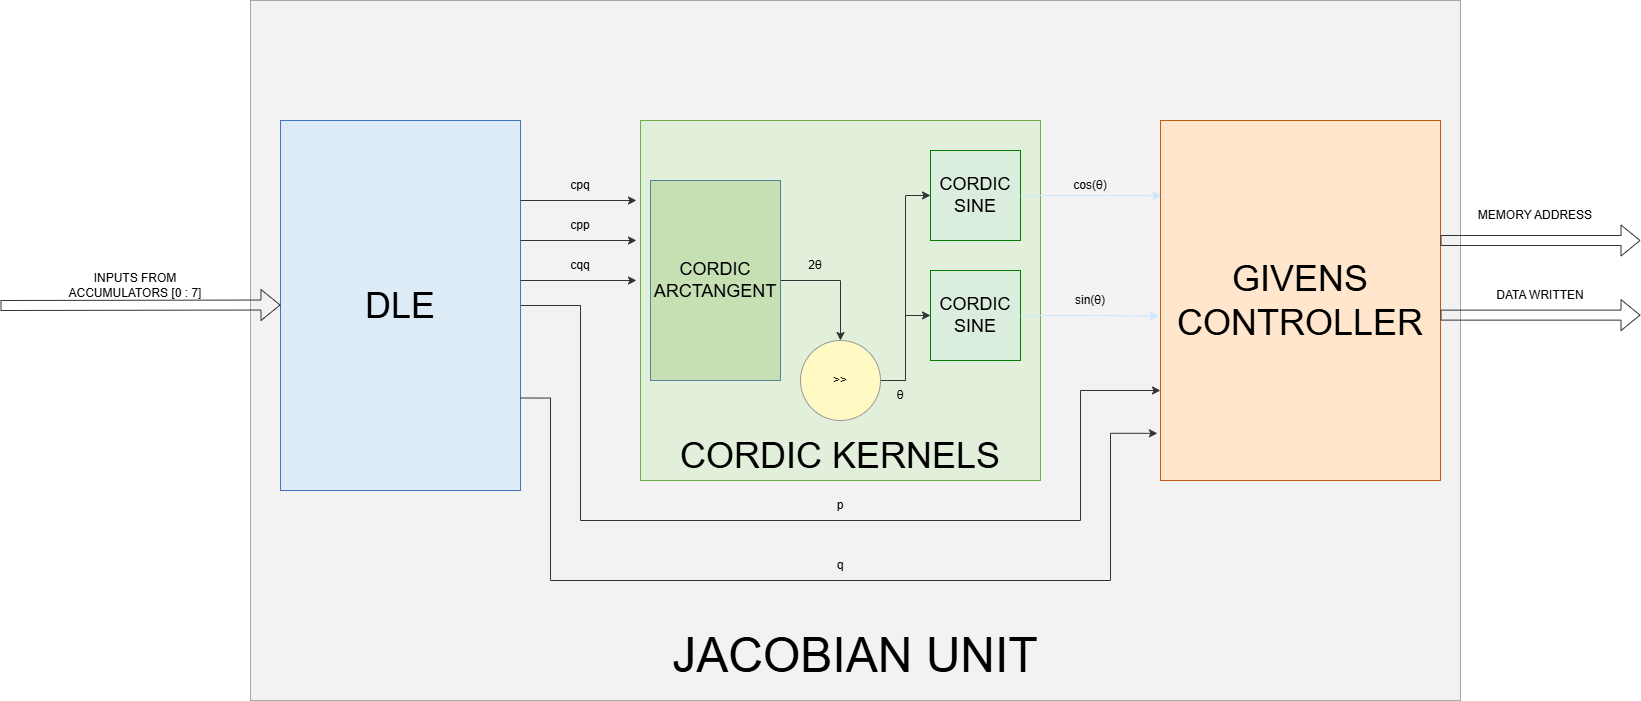
\includegraphics[scale = 0.3]{Figures/Jacobian Unit.png}}
	\caption{Jacobian Unit Architecture}
	\label{fig:jacobian unit architecture}
\end{figure}

\subsection{Data Lookup Engine (DLE)}
The Data Lookup Engine (DLE) is a unique architectural innovation in Manojavam, specifically designed to identify the largest off-diagonal entry in the symmetric covariance matrix $C$, which is the target of each Jacobi sweep. Unlike conventional designs that rely on off-chip memory or multiple on-chip reads to traverse the matrix and extract this value, the DLE operates in-line with the accumulation path of the matrix multiplication unit. As partial sums for each matrix tile are generated during block streaming multiplication, the DLE snoops into these intermediate values and selectively captures the relevant ones based on the row-block and column-block identifiers.

To ensure that only valid off-diagonal elements cpq are considered, the DLE incorporates logic to ignore diagonal entries ($c_{pp}$, $c_{qq}$) and focuses only on entries where $p \neq q$. For example, during the accumulation of row block $R_{0}$, only entries from accumulators corresponding to columns 1 through $N$ are considered, with accumulator 0 (holding $c_{pp}$) explicitly excluded. This dynamic filter is implemented using row-wise masking and loop counters governed by the Jacobian Controller.

The DLE maintains a running maximum register, which stores the current best candidate $c_{pq}$ and its associated diagonal elements $c_{pp}$, $c_{qq}$, as well as the corresponding indices $p$ and $q$. These values are updated if a newly received cpq is of greater absolute magnitude than the current maximum. Once a complete row sweep is done, the DLE asserts a ready flag and outputs the final triplet. This mechanism eliminates the need for matrix reads post-accumulation and tightly couples the matrix traversal logic with the systolic dataflow, making it highly efficient in both time and energy.

\subsection{CORDIC Kernels}
After the DLE has identified the indices $(p, q)$ and corresponding values $c_{pq}$, $c_{pp}$, and $c_{qq}$, the next stage involves computing the rotation angle $\theta$ required to construct the Givens rotation matrix $R$. This is done using the equation:

\begin{equation}
	\theta = \frac{1}{2}\arctan(\frac{2.c_{pq}}{c_{pp} - c_{qq}})
	\label{eq:rotation-angle-equation}
\end{equation}

This computation typically involves a floating-point division and arctangent operation, which are hardware-expensive. Instead, Manojavam employs CORDIC (Coordinate Rotation Digital Computer) kernels — a class of shift-and-add algorithms that efficiently compute trigonometric functions using only adders, shifters, and a lookup table.

The CORDIC engine is implemented as a 3-stage pipeline:
\begin{itemize}
	\item Stage 1 computes the arctangent of the normalized input.
	\item Stage 2 and 3 compute the sine and cosine of the resulting angle using vector rotation mode. 
\end{itemize}

These kernels work in fixed-point arithmetic, carefully scaled to match the datapath width of Manojavam while preserving numerical stability. Because of pipelining, a new angle can be fed into the CORDIC engine every few clock cycles, and once the latency is absorbed, the unit can achieve near-one-angle-per-cycle throughput. This design is ideal for iterative eigendecomposition, where hundreds of such angles may be computed across multiple Jacobi sweeps.

The $sin(\theta)$ and $cos(\theta)$ values are then forwarded to the Givens Engine, which uses them to construct the sparse rotation matrix.

\subsection{Givens Engine}
The Givens Engine is responsible for generating and storing the actual Givens rotation matrix $R$ using the rotation angle $\theta$. In the Jacobi method, the Givens matrix is an identity matrix with four modified elements at $[p][p]$, $[q][q]$, $[p][q]$, and $[q][p]$, which are set to:
\begin{enumerate}
	\item $R_{pp} = R_{qq} = cos(\theta)$
	\item $R_{pq} = sin(\theta)$
	\item $R_{qp} = -sin(\theta)$
\end{enumerate}

This localized modification is sufficient to apply a plane rotation in the $(p,q)$ subspace of the matrix, progressively zeroing out the off-diagonal term $c_{pq}$. The Givens Engine stores this matrix in a dual-port RAM, enabling simultaneous read and write operations during iterative construction and rotation phases. This storage structure is accessed by downstream matrix multiplication units for computing:
\begin{equation}
	C^{'} = R^{T}CR
\end{equation}

\begin{equation}
	V = VR
\end{equation}

The Givens Controller synchronizes matrix updates and triggers operand movement within the memory hierarchy. It generates select signals to update only relevant portions of the Givens matrix, thereby avoiding unnecessary re-initialization. Once the matrix is ready, a mode signal is broadcast to all computational units, switching the pipeline from covariance accumulation to rotation mode.

To minimize performance overhead, the engine also preloads the next Givens rotation during the computation of the current matrix transformation, enabling overlap of angle generation and matrix rotation — a technique analogous to prefetching in cache systems.

\section{Cache Subsystem}
Efficient memory access plays a critical role in sustaining the performance of high-throughput accelerators. In Manojavam, where multiple 4×4 systolic arrays operate in parallel, the design of the memory subsystem is crucial for maintaining computational flow without stalling. To support continuous and parallel tile streaming across compute stages, Manojavam implements a dual-tier cache hierarchy—consisting of L1 and L2 caches—architected specifically to match the operand reuse patterns that arise in block-wise matrix multiplication.

The left-hand side (LHS) operands, such as the rows of $X^{T}$ during covariance matrix computation or $R^{T}$ during rotations, are typically reused across multiple columns or matrix blocks. This temporal locality makes them good candidates for shared caching. Accordingly, all LHS operands are stored in a shared L1 cache, which is accessible to all eight systolic arrays through a broadcast-style access network. This shared architecture reduces memory footprint, eliminates unnecessary duplication of frequently used data, and simplifies coherency management for read-only accesses. The shared cache also includes address decoding and basic arbitration logic to allow synchronized reads from multiple consumers.

In contrast, the right-hand side (RHS) operands—including the columns of $X$, the evolving covariance matrix $C$, or the rotation matrix $R$—are typically unique to each systolic array during a particular compute cycle. These operands do not exhibit the same reuse pattern and are thus stored in private L1 caches, with each cache directly connected to one of the eight systolic arrays. This private caching scheme eliminates the need for read arbitration, enables concurrent data delivery, and supports tile-specific prefetching. Each private cache is configured to hold an entire 4×4 operand tile in a row-aligned format, enabling burst-mode reads to feed systolic inputs efficiently.

To optimize data delivery, the cache stores each operand tile in a row-major layout rather than as a raw matrix. This means each row of the 4×4 tile is stored contiguously, allowing the systolic array to receive an entire row of inputs in a single read cycle instead of multiple sequential accesses. By reducing the number of memory fetches from four to one per row, this approach significantly improves data throughput, reduces latency, and better aligns with the streaming nature of the systolic array’s pipeline.

All L1 caches—both shared and private—are backed by a common L2 memory pool, implemented as a dual-ported block RAM module or connected externally via a DDR3 memory interface. This L2 layer serves as the staging area for incoming operand tiles and also receives the accumulated results post-computation. A dedicated memory controller coordinates requests from the cache complex and enforces proper sequencing for tile fetch and write-back operations. To reduce memory bandwidth pressure and prevent redundant data movement, Manojavam employs selective cache write policies tailored to the two major computation phases.

During covariance matrix computation, a write-around policy is used for the RHS caches. In this policy, new tiles are written directly to memory without allocating space in the cache unless the data is expected to be reused. This minimizes cache pollution and allows each private cache to retain active working tiles without being overwritten by one-time-use data.

In the rotation phase, a write-validate policy is enforced, especially for matrix $C$ and the evolving eigenvector matrix $V$. This policy ensures that when matrix updates are written to memory, the corresponding cache entries are marked valid, but no fetch-on-write is triggered. This reduces unnecessary memory traffic while still maintaining coherency. The system relies on the fact that the MM Engine overwrites the same tile locations in a predictable schedule, making manual validation sufficient for correctness.

Tile streaming in this memory hierarchy is managed via a controller-driven tile scheduler, which issues operand fetch signals to the caches in a fixed loop structure. This streaming-friendly model avoids complex memory dependency tracking and supports pipeline-friendly operand delivery to the systolic arrays. Furthermore, by isolating frequently reused operands from ephemeral ones, the design achieves a balance between temporal locality exploitation and parallel access concurrency, both of which are critical in matrix-intensive computation.

The overall memory system is designed to scale with matrix size, supporting tile dimensions beyond the capacity of L1 caches by fetching on demand and buffering partial results for accumulation. It minimizes idle cycles in the datapath, maintains high utilization of the systolic arrays, and simplifies the scheduling logic by clearly separating cache responsibilities according to operand behavior. This architecture, while lightweight in its logic and buffering requirements, forms a central enabler of Manojavam’s streaming and reuse-aware compute strategy.   

\section{Controller Design and Hierarchy}
The efficient operation of the Manojavam PCA accelerator heavily relies on a well-structured controller hierarchy that orchestrates data flow, synchronization, and computation across multiple compute units and memory subsystems. The hierarchy is designed to modularize control responsibilities, simplify synchronization, and enable scalable management of parallel processing elements. The controller hierarchy consists of four primary levels:

\subsection{Top-Level Controller}
At the apex of the control architecture lies the Top-Level Controller, which functions as the master coordinator for the entire design. Its primary responsibility is to synchronize all subordinate controllers, ensuring smooth handshaking and timing alignment between the different units—namely, the shared LHS cache controller, the private RHS cache controller complex, and the Jacobian Unit controller. The top-level controller orchestrates the overall flow of computation phases, triggers operand fetch and store operations, and manages global start, stop, and reset signals. By maintaining a centralized state machine, this controller ensures that the system operates in a lockstep manner, preventing data hazards and ensuring consistent data availability across all compute pipelines.

\subsection{LHS Shared Cache Controller}
The LHS Shared Cache Controller is responsible for managing all operations related to the left-hand side (LHS) shared cache. This includes handling broadcast reads to multiple systolic arrays, address decoding, cache coherence management for read-only data, and arbitration for simultaneous access requests. Given that the LHS operands exhibit high temporal reuse and are shared across all eight systolic arrays, this controller plays a critical role in reducing redundant memory traffic and maintaining consistent operand delivery. It schedules tile fetches from the L2 memory into the shared cache and coordinates cache line validation to ensure the freshest data is available to the compute units.

\subsection{Private RHS Cache Controller Complex}
The Private RHS Cache Controller Complex comprises eight independent private cache controllers, each dedicated to managing one of the eight private RHS caches linked to the individual systolic arrays. Each private cache controller handles local operand prefetching, cache line allocation, and write-back policies tailored to the right-hand side (RHS) operands that are unique per systolic array during computation. This modular organization enables concurrent and conflict-free memory accesses, as each controller operates autonomously with minimal synchronization overhead. The complex also enforces the selective write-around and write-validate policies, optimizing cache utilization based on operand reuse characteristics in covariance and rotation phases.

\subsection{Jacobian Controller}
The Jacobian Controller oversees the operation of the Jacobian Unit, which is responsible for implementing the Jacobi eigendecomposition algorithm during the PCA process. This controller manages iterative sweep operations, controls rotation matrix generation via CORDIC engines, and coordinates data movement between the rotation unit and the matrix multiplication engine. It synchronizes the execution of Givens rotations and ensures correct sequencing of eigenvector updates. By tightly integrating with the top-level controller, the Jacobian Controller maintains coherent operation between the covariance computation phase and the rotation phase, enabling smooth pipeline transitions.

\begin{comment}
\section{Contents of this Chapter}
This chapter should contain the following sections and subsections in detail.
\begin{enumerate}
\item Specifications for the Design
\item Pre analysis work for the design or Models used
\item Design methodology in detail
\item Design Equations
\item Experimental techniques (if any)
\end{enumerate}
Apart from the aforementioned sections, you can add sections as per the requirements of the project in consultation with your guide.
\end{comment}

Chapter 3 presents the comprehensive design methodology and specifications that underpin both the FPGA Architectural Exploration and the development of the Manojavam PCA accelerator. It begins by detailing the specific design requirements and objectives for evaluating diverse FPGA architectures using the VTR toolchain, followed by the modeling approaches employed to accurately represent targeted FPGA configurations. The chapter outlines the systematic methodology adopted to perform architectural exploration, including synthesis, placement, and routing workflows, alongside the critical performance and area analysis metrics supported by relevant equations. The focus then shifts to the architectural design of the Manojavam accelerator, describing its core components in detail — the matrix multiplication engine, which leverages multiple 4×4 systolic arrays for high-throughput matrix operations; the Jacobian unit, responsible for eigendecomposition via Jacobi rotations; and the cache subsystem, architected to optimize operand reuse and data streaming. Finally, the controller hierarchy is elaborated, highlighting the modular control scheme that ensures synchronized operation and efficient data flow across the compute and memory units. Together, these sections form the foundation for both the FPGA exploration and accelerator implementation, linking theoretical design choices with practical hardware realization.

\begin{comment}
\section{Paraphrasing}
When you paraphrase a written passage, you rewrite it to state the essential ideas in your own words. Because you do not quote your source word for word when paraphrasing, it is unnecessary to enclose the paraphrased material in quotation marks. However, the paraphrased material must be properly referenced because the ideas are taken from someone else whether or not the words are identical. 

Ordinarily, the majority of the notes you take during the research phase of writing your report will paraphrase the original material. Paraphrase only the essential ideas. Strive to put original ideas into your own words without distorting them."

\section{Quotations}
When you have borrowed words, facts, or idea of any kind from someone else's work, acknowledge your debt by giving your source credit in footnote (or in running text as cited reference). Otherwise, you will be guilty of plagiarism. Also, be sure you have represented the original material honestly and accurately. Direct word to word quotations are enclosed in quotation marks."

\vspace{0.75cm}

 \textbf{The chapters should not end with figures, instead bring the paragraph explaining about the figure at the end followed by a summary paragraph.}
\end{comment}

\begin{comment}
After elaborating the various sections of the chapter (From Chapter 2 onwards), a summary paragraph should be written discussing the highlights of that particular chapter. This summary paragraph should not be numbered separately. This paragraph should connect the present chapter to the next chapter.  
\end{comment}

%Chapter 4
\chapter{Implementation}
Robust implementation frameworks form the foundation of both architectural exploration and hardware accelerator development. For the FPGA design exploration project, the Verilog-to-Routing (VTR) toolchain is deployed within a Docker-based environment to ensure reproducibility and consistency. Benchmark circuits are synthesized using Yosys and ABC, followed by placement, routing, and detailed metric analysis through VPR. In parallel, the Manojavam PCA accelerator is realized through a modular RTL design approach, incorporating optimized matrix multiplication engines, cache subsystems, and synchronized controller hierarchies. This chapter presents the systematic workflow and technical steps followed in translating both conceptual designs into functioning and analyzable implementations.

\begin{comment}
\indent\indent From Chapter 2 onwards, every chapter should start with an introduction paragraph. This paragraph should brief about the flow of the chapter. This introduction can be limited within 4 to 5 sentences. The chapter heading should be appropriately modified (a sample heading is shown for this chapter).But don't start the introduction paragraph in the chapters 2 to end with "This chapter deals with....". Instead you should bring in the highlights of the chapter in the introduction paragraph. 
\end{comment}

\section{Docker Container for VTR}
The Verilog-to-Routing (VTR) toolchain, which encompasses multiple complex software components including synthesis, technology mapping, packing, placement, and routing tools, requires a carefully configured software environment to function correctly. To simplify environment setup and ensure reproducibility, we leveraged a pre-built Docker container specifically designed for VTR execution. This approach abstracts away the challenges of dependency management, version compatibility, and operating system configurations, enabling a seamless and consistent platform for architectural exploration.

From an implementation perspective, the Docker container encapsulates the entire VTR toolchain along with all necessary dependencies, including required libraries, compilers, and scripts. By using Docker, the VTR environment becomes portable and can be deployed on any host system that supports Docker, whether it is a local workstation, a remote server, or a cloud-based instance. This containerized setup eliminates the need for manual installation or configuration of individual components, which can be error-prone and time-consuming.

To use the Docker container, we pulled the official or community-maintained VTR image from a Docker repository. The container was then instantiated on the target machine, providing an isolated and consistent execution environment. Input files such as architecture XML descriptions, benchmark Verilog files, and configuration scripts were mounted as volumes inside the container, allowing easy access and modification without rebuilding the image.

The container also facilitates batch automation by allowing execution of shell scripts and experiment workflows inside a controlled environment. This is particularly beneficial when running large-scale FPGA architectural explorations requiring multiple iterations of synthesis, packing, placement, and routing. Additionally, Docker’s resource management options enable allocation of CPU cores and memory to the container, ensuring predictable performance and efficient utilization of hardware resources.

Overall, using a Docker container for VTR significantly improved the reliability and reproducibility of our architectural exploration experiments. It simplified collaboration and sharing of the experimental setup with other researchers, and reduced the overhead of troubleshooting environment-related issues. This containerized approach aligns well with best practices in modern hardware research workflows, where toolchain consistency and portability are crucial.

\section{Architectural Description}
The Verilog-to-Routing (VTR) framework enables architectural exploration of FPGA designs through configurable XML-based architecture description files. These files define the fundamental components of the FPGA fabric—such as logic blocks, routing architecture, I/O configurations, and DSPs—and form the foundation for synthesis, placement, and routing experiments. For this project, three distinct FPGA architectures were selected and implemented: Intel Stratix-10 (as a representative of commercial high-performance FPGAs), a custom 4-bit Single Carry Chain architecture, and a 4-bit Double Carry Chain architecture. Each architecture was described in its respective XML file, guided by the syntax and schema provided in the VTR Architecture Reference Manual.

\subsection{Intel Stratix-10 Architecture}
The Stratix-10 architecture description was adapted from the official Stratix10 architecture XML file in the VTR repository. This model includes a wide range of hardened elements including DSP blocks, dual-port RAMs, and fracturable logic elements. The configurable logic blocks (CLBs) consist of Adaptive Logic Modules (ALMs), each capable of handling variable input widths and logic functions. The routing fabric is highly segmented and features diverse switch block patterns to mimic the physical routing complexities found in real Intel FPGAs. From an implementation perspective, this architecture provides a high-performance baseline for benchmarking, reflecting a production-grade FPGA with mature logic synthesis capabilities.

\subsection{4-Bit Single Carry Chain Architecture}
The single chain carry architecture models a lightweight, arithmetic-friendly FPGA optimized for small-bitwidth operations. Implemented in the 4bit-adder-single-chain-arch.xml file, this design features logic blocks with embedded 4-bit adders configured in a serial carry propagation style. Each logic block supports straightforward arithmetic operations and basic logic functions, with carry-in and carry-out ports connected in a linear fashion. The design focuses on compact resource allocation and favors applications involving low-precision neural network computations or signal processing tasks. This architecture prioritizes minimum delay in bit-serial arithmetic and efficient area usage.

\subsection{4-Bit Double Carry Chain Architecture}
Expanding upon the single chain model, the double chain carry architecture—described in 4bit-adder-double-chain-arch.xml—implements dual carry chains within each logic block. This allows parallel evaluation of two 4-bit additions or partial products, enhancing throughput for arithmetic-heavy workloads. Each logic element includes two cascaded carry propagation paths and supports conditional logic evaluation based on runtime selection of carry routes. This architecture is particularly well-suited for accelerating MAC (multiply-accumulate) operations, making it highly applicable for machine learning accelerators and DSP workloads. Routing resources were adjusted accordingly to support higher interconnect demand due to parallelism.

\section{Benchmark Creation}
To evaluate the performance and suitability of the target FPGA architectures modeled in VTR, a diverse set of Verilog-based benchmark circuits was created. These benchmarks were selected to stress arithmetic and logic capabilities, especially in the context of low-bitwidth machine learning primitives and digital signal processing (DSP) functions. The primary benchmark types include adder tree networks, FIR filters, and modified FIR filters with custom arithmetic structures.

\subsection{Adder Tree Benchmarks}
Adder tree benchmarks serve as fundamental arithmetic units and are frequently encountered in accumulation operations within MAC units, dot products, and tree-based summations. The benchmarks were implemented using combinational adder trees of varying depths and bit-widths. Each benchmark was unrolled into either 2-level or 3-level structures, consisting of multiple full adders arranged in a tree-like hierarchy. These benchmarks provided insights into carry propagation, logic packing efficiency, and routing overheads in each FPGA architecture.

\subsection{FIR Filter Benchmarks}
Finite Impulse Response (FIR) filters are core components in DSP workloads and provide a structured combination of multipliers and adders. Standard FIR benchmarks were written in Verilog to model a multiply-and-accumulate pipeline. Variants were created for different tap counts (e.g., 4-tap, 8-tap), and both pipelined and unpipelined versions were generated. Multiplications were performed using the standard \textbf{(*)} operator, which allowed synthesis tools to map them to either LUT-based or DSP-based implementations depending on the target architecture. These filters test both arithmetic depth and the interconnection complexity of logic blocks.

\subsection{Modified FIR Benchmarks with Wallace Tree Multipliers}
To emulate the structure of arithmetic accelerators and explore resource-level optimization, modified FIR benchmarks were created by replacing the built-in multiplication operator with an explicitly constructed Wallace Tree multiplier. The Wallace Tree multiplier was designed in Vivado using 1-bit multipliers and structured carry-save adder networks, enabling precise control over the hardware implementation.

A dedicated Python script was developed to automate the integration of this Wallace Tree design into all existing FIR filter benchmarks. This script scanned the original FIR Verilog files, identified the multiplication expressions, and replaced them with instances of the custom Wallace Tree module. It then generated new benchmark Verilog files with these modifications, which were placed in a separate directory for clarity and version control. Each modified benchmark preserved the original filter behavior but exhibited different synthesis and placement characteristics, allowing for a more nuanced comparison of how each target FPGA architecture handled complex arithmetic datapaths.

These benchmark variants—standard, pipelined, and Wallace Tree-based—were compiled into a unified test suite and systematically mapped to all three target architectures using automated flow scripts. This ensured consistent synthesis conditions and enabled direct performance comparisons across architectural designs.

\section{Shell Automation Scripts}
Mapping each benchmark design to the various FPGA architecture descriptions using the VTR flow is a multi-step process involving synthesis, BLIF generation, packing, placement, routing, and result analysis. Manually repeating these steps for every benchmark and architecture combination becomes highly tedious, especially when dealing with numerous benchmark variants and multiple architecture XML files. To overcome this challenge and eliminate the need for repeated terminal commands, automation scripts were developed to handle the entire benchmarking process.

These shell scripts enabled full traversal of all benchmark files and systematically mapped them to each of the target FPGA architectures. The scripts internally invoked Yosys to synthesize each Verilog benchmark into a BLIF representation, followed by automatic invocation of VPR using the appropriate architecture XML files. The resulting timing, area, and routing reports were generated and logged in structured output folders for each benchmark-architecture pair.

By automating the architecture-benchmark mapping process, the scripts significantly reduced manual intervention, ensured consistency in execution, and sped up the benchmarking effort. The generated reports were organized for post-processing and allowed for easy retrieval and comparison across architecture variants. This automation proved instrumental in enabling rapid design space exploration and in maintaining reproducibility across experimental runs.

\section{BLIF File Generation using Parmys and ABC}
In the FPGA architectural exploration flow using VTR, generating BLIF (Berkeley Logic Interchange Format) files is a crucial intermediate step that connects the high-level Verilog design of a benchmark to the architectural specification of a target FPGA. This transformation is handled by a synthesis pipeline involving Parmys and ABC, which together perform elaboration, optimization, and technology mapping of the Verilog source.

Parmys is a lightweight and modular front-end Verilog parser and elaboration tool developed as a plugin to interface with the VTR ecosystem. Unlike traditional synthesis tools, Parmys focuses on quickly parsing behavioral and structural Verilog, flattening the hierarchy, and converting the design into an intermediate gate-level netlist that is suitable for logic optimization and mapping. It is designed with integration into VTR in mind, ensuring that the logic structures it produces align closely with VTR's architectural models, particularly for LUT-based FPGA fabrics.

Once the Verilog benchmark is parsed and elaborated by Parmys, the resulting netlist is handed over to ABC, a powerful tool for logic synthesis and technology mapping. ABC optimizes the logic through a series of rewriting, resubstitution, and balancing steps, and then maps the optimized logic to a target logic family, typically defined by K-input LUTs (e.g., 4-LUTs or 6-LUTs), based on the architecture definition. This technology-mapped representation is then output as a .blif file, which serves as the input to the VPR (Versatile Place and Route) tool in the next phase of the flow.

While the architectural XML description is not directly consumed during BLIF generation, it influences the synthesis constraints. For example, if the target FPGA architecture supports only 4-input LUTs (as in the 4-bit adder architectures), ABC is invoked with a corresponding LUT size parameter to ensure the output is structurally compatible with the architecture.

From an implementation standpoint, the synthesis flow begins by passing each Verilog benchmark through Parmys, which performs parsing and elaboration. The intermediate design is then piped into ABC, with appropriate mapping commands, to produce the final .blif file. This entire process is integrated into automation scripts to handle multiple benchmarks across various target architectures. The resulting BLIF files serve as architecture-aware netlists that are used by VPR for placement, routing, and physical resource analysis.

This Parmys+ABC synthesis flow ensures consistency, automation, and compatibility across the exploration pipeline, enabling rapid evaluation of benchmark behavior on custom FPGA architectures.

\section{VPR Pack, Place \& Route}
After generating the BLIF netlist using Parmys and ABC, the next phase of the VTR flow involves performing pack, place, and route operations using the Versatile Place and Route (VPR) tool. This process translates the abstract netlist into a concrete physical mapping on the FPGA grid defined by the target architecture.

The first stage, packing, groups logical elements such as LUTs, flip-flops, and carry logic into clusters called logic blocks. VPR uses the architecture XML file to determine the permissible packing patterns, which differ across the Stratix-10 and the custom 4-bit carry chain architectures. This step ensures that logic elements are organized into valid cluster configurations before proceeding to physical layout.

Once packing is completed, VPR moves to placement, where each packed cluster is assigned a position on the FPGA fabric. The placement algorithm attempts to minimize critical path delay and wire length, taking into account the architecture’s grid layout and connectivity constraints. Placement quality directly impacts timing, making this stage essential for performance optimization.

The final step is routing, in which the placed logic blocks are interconnected using the FPGA's routing resources. VPR constructs routing trees that obey the architecture-defined switch boxes and channel widths. Successful routing ensures that all signal paths are physically realizable on the target fabric. After routing, VPR generates detailed timing, area, and wire length reports, which are used for evaluating the effectiveness of the architecture when mapped with a specific benchmark.

This pack, place, and route sequence completes the physical implementation of a benchmark on a given FPGA model, enabling quantitative comparison between architectures under consistent workloads.

\section{Architecture Timing and Area Analysis}
Once the VPR pack, place, and route stages are completed, the final step in the implementation flow involves analyzing the timing and area characteristics of each benchmark mapped to a target architecture. These metrics are crucial for evaluating architectural suitability in the context of real-world workloads, particularly in latency- or resource-constrained environments such as machine learning accelerators.

VPR automatically generates detailed reports during the post-analysis phase, including metrics such as critical path delay, total wire length, and logic block utilization. These values reflect the overall timing performance and silicon area efficiency of the FPGA implementation. The critical path delay serves as the primary indicator of the maximum achievable clock frequency, while area metrics such as the number of LUTs, flip-flops, and routing channels used help quantify the hardware footprint of each benchmark.

Given the large number of benchmark-architecture pairings, manually parsing each VPR-generated log file for timing and area statistics would be extremely tedious and error-prone. To address this, a set of shell scripts was developed to recursively traverse the benchmark result directories, extract the relevant performance metrics from the VPR output logs, and tabulate them in a structured format. This automation not only accelerated the evaluation process but also ensured consistency and reproducibility across experiments.

Through this scripted post-processing pipeline, comprehensive architectural comparisons were made possible, enabling insights into how each target FPGA configuration—Stratix-10, 4-bit single carry chain, and 4-bit double carry chain—responds to a diverse suite of logic-intensive benchmarks.

\section{Target FPGA Platform for Manojavam}
The hardware realization of the Manojavam accelerator was implemented on the AMD Artix-7 XC7A35T-CPG236 FPGA, a mid-range device that strikes a practical balance between resource availability, cost-efficiency, and power consumption. As part of the Artix-7 family, this chip offers 33,280 logic cells, 90 DSP slices, 50 BRAM blocks (each 36 Kb), and up to 106 general-purpose I/Os—sufficient to accommodate complex designs involving parallel compute engines, pipelined control, and multi-level memory hierarchies\cite{chap4-1}.

This specific FPGA supports a core voltage of 1.0V and configurable I/O voltages ranging from 1.2V to 3.3V, enabling flexible interfacing and integration with external memory and debug modules.

A key reason behind choosing the XC7A35T was its classification as a mid-tier FPGA platform—not as resource-rich as high-end Virtex or Zynq devices, but still capable of supporting non-trivial, computation-heavy accelerators like Manojavam. Successfully implementing a design of this scale and performance complexity on such a constrained FPGA underscored both the architectural efficiency of the accelerator and the strength of its RTL pipeline design. The ability to achieve high throughput (~2 GOPS) on this device reinforces the viability of deploying Manojavam on cost-sensitive or power-limited platforms in real-world scenarios.

The design was built, simulated, and deployed using AMD Vivado ML Edition 2024.1, which provides an optimized development environment for ML-centric workloads and FPGA-based accelerators. This toolchain offered improved synthesis quality, accurate post-implementation timing analysis, and integrated power estimation—critical for validating the resource and thermal characteristics of the design. Vivado’s hierarchical project structure, IP integration capabilities, and native simulation support enabled modular development of Manojavam’s matrix engine, control hierarchy, and cache system. Additionally, the enhanced DSP inference optimizations in the 2024.1 release helped to better utilize the FPGA’s limited DSP slices in the systolic array implementation.

Overall, the Artix-7 platform served as a compelling testbed, proving that large-scale ML accelerators can be both prototyped and meaningfully evaluated on affordable, mid-class FPGAs.

\section{RTL Entry and Behavioral Simulation}
The RTL (Register Transfer Level) design of Manojavam was written using Verilog HDL, with a modular structure to represent each functional block of the accelerator. Modules were created for the matrix multiplication engine, systolic arrays, cache subsystems, rotation unit, and controller hierarchy. Each module was kept functionally independent to allow easy debugging, simulation, and reuse. The design followed a top-down integration strategy where smaller blocks were tested individually before being connected together in the top-level module.

For functional verification, behavioral simulation was carried out using the Vivado Simulator. Testbenches were written for each module to verify their input-output behavior. For instance, the matrix multiplication engine was tested using simple matrix tiles, and expected outputs were manually calculated and verified. Similarly, cache controllers were simulated to confirm proper data movement and synchronization between memory levels. All modules were first simulated independently and later tested as part of an integrated top-level simulation.

The goal of this stage was not to optimize timing or synthesis yet, but to ensure that the logic described in Verilog functioned as intended. Waveform viewers in Vivado were used extensively to track signal transitions and debug potential design mismatches. Once behavioral simulation showed correct functionality, the design moved to synthesis and implementation stages.

This simulation-driven approach helped catch errors early and saved time during later stages of the FPGA workflow.

\section{Xilinx Design Constraints}
Design constraints are a vital part of implementing any FPGA-based system, as they serve to bridge the gap between a functional RTL design and its successful realization on physical hardware. In the context of the Manojavam accelerator, Xilinx Design Constraints (XDC) were used to specify essential aspects of the design such as pin assignments, clock configurations, and layout planning. These constraints helped ensure correct electrical behavior, reliable timing performance, and efficient use of FPGA resources throughout the implementation process.

\subsection{I/O Constraints}
I/O constraints define how the design’s inputs and outputs are mapped to the physical pins on the FPGA package. For Manojavam, all critical ports—including operand inputs, control signals, and outputs—were carefully assigned to specific pins on the Artix-7 FPGA. Along with pin location, additional attributes like voltage levels, I/O standards, and drive strength were specified to match external components and comply with electrical requirements. These I/O constraints ensured stable communication between the FPGA and its surrounding system environment.

\subsection{Clock Constraints}
Proper timing behavior is critical in digital systems, making clock constraints one of the most important parts of FPGA implementation. In Manojavam, constraints were used to define the primary system clock, along with its expected period. The design also incorporated timing relationships between the clock and the arrival or departure of data on specific IOs. These constraints enabled Vivado’s synthesis and implementation tools to analyze and optimize the design’s timing paths, ensuring that all internal components operated reliably at the target frequency without timing violations.

\subsection{PBlock Floorplanning Constraints}
To improve modularity and manage routing congestion, floorplanning constraints were applied using placement blocks, or PBlocks\cite{chap4-2}. These constraints defined specific regions on the FPGA fabric where particular components of the design—such as systolic arrays, cache systems, or controller modules—would be placed. Assigning different parts of the design to dedicated regions reduced routing conflicts and helped achieve better timing closure. PBlocks also provided a clearer physical layout, making the design easier to analyze and debug.

Together, these constraint categories played a crucial role in shaping the final implementation of the Manojavam accelerator. By clearly defining how the design should interface with the FPGA and how it should be arranged internally, the use of design constraints ensured performance consistency, predictable behavior, and a smooth transition from simulation to hardware.

\section{Synthesis}
Synthesis is a critical phase in FPGA design as it translates high-level RTL code into a gate-level representation compatible with the hardware fabric. For Manojavam, synthesis was performed using the AMD Vivado 2024.1 ML Edition, targeting the Artix-7 xc7a35tcpg236 FPGA. This step maps Verilog constructs to available FPGA primitives such as LUTs, flip-flops, BRAMs, and DSP slices, allowing the design to be implemented on physical silicon. It also provides valuable insight into how efficiently the design utilizes hardware resources, how much power it may consume, and whether it can meet required timing constraints.

\subsection{Post Synthesis Simulations}
Once synthesis was complete, post-synthesis simulations were performed to validate that the mapped gate-level netlist still preserved functional correctness. These simulations accounted for delays introduced by synthesis optimizations and resource mapping, ensuring no unintended logic behavior had been introduced. The same testbenches from behavioral simulation were reused at this stage, but the simulation now reflected a more realistic, timing-aware model of the hardware. Any mismatches between RTL and post-synthesis behavior were carefully analyzed and fixed before proceeding further.

\subsection{Utilization and Power Reports}
Vivado’s synthesis process generated detailed utilization reports, summarizing how many LUTs, flip-flops, DSPs, BRAMs, and IOs were consumed. These metrics were critical in understanding the resource footprint of Manojavam’s architecture. In addition, Vivado provided power analysis reports estimating both dynamic and static power consumption. This data helped evaluate the efficiency of the design and highlighted potential hotspots or overuse of resources that could lead to overheating, a known challenge in the earlier iterations of Manojavam.

\subsection{Timing Summaries}
Finally, timing summaries were reviewed to assess whether the design could operate at the target clock frequency without setup or hold violations. Vivado generated timing analysis results such as Worst Negative Slack (WNS), Total Negative Slack (TNS), and achieved clock frequency. These results determined whether the system was capable of running at its intended performance. For Manojavam, achieving timing closure was essential to maintain high throughput for matrix operations and maintain synchronization across the systolic arrays, cache controllers, and control logic.

\section{Implementation}
FPGA implementation is the final and critical step that translates a verified RTL design into a physical configuration that can be programmed onto the chip. While synthesis transforms the design into logical primitives, the implementation process performs placement and routing, assigning these primitives to specific physical locations and connecting them via the FPGA’s interconnect. This step ensures that the design meets timing, area, and resource constraints under real-world operating conditions. For a complex architecture like Manojavam, successful implementation is key to achieving predictable performance and energy efficiency on the target Artix-7 FPGA.

\subsection{Post Implementation Simulations}
After implementation, it is crucial to verify that the placed and routed design maintains its functional correctness and adheres to the expected timing. Post-implementation simulation uses timing-annotated netlists that reflect real propagation delays, allowing accurate observation of timing behavior across all critical paths. In the Manojavam project, these simulations were used to validate the system’s functional performance under timing constraints and to catch any issues not visible during earlier behavioral or post-synthesis simulation stages. This step helped confirm the design’s reliability at its target operational frequency.

\subsection{Utilization and Power Reports}
Once the design is implemented, Vivado generates detailed reports on FPGA resource usage and power consumption. The utilization report includes information about the number of LUTs, flip-flops, DSP slices, and BRAMs used, which is important for analyzing the efficiency of the hardware architecture. For Manojavam, these insights were particularly useful in evaluating how effectively each subsystem—such as the matrix multiplication engine and memory units—fit into the mid-range Artix-7 FPGA fabric.

Similarly, the power report provides a breakdown of dynamic and static power consumption. This includes contributions from logic, signal transitions, clocking, and IOs. The power analysis helped assess the overall energy profile of the Manojavam accelerator and served as a reference point for identifying hotspots and areas of potential optimization in future iterations of the design.

\section{Openlane ASIC Implementation}
While the Manojavam accelerator was primarily designed and tested on an FPGA platform, exploring its implementation using an ASIC design flow provides critical insights into its scalability, performance, and suitability for future chip fabrication. OpenLane, an open-source ASIC toolchain built on top of tools like Yosys, OpenROAD, and Magic, offers a fully automated RTL-to-GDSII flow for synthesizing and realizing digital designs in silicon. For Manojavam, the OpenLane flow enabled a practical understanding of area, power, and timing in the context of custom silicon. This ASIC-level evaluation helped analyze how Manojavam might perform in a real-world application-specific integrated circuit environment, offering a glimpse into its potential as a domain-specific ML accelerator chip.

\subsection{Openlane RTL Entry and Configuration File}
The implementation process begins with the entry of Verilog RTL into the OpenLane flow. The source files describing the Manojavam subsystems—matrix engine, Jacobian unit, memory controllers, etc.—were consolidated and referenced in the configuration file (config.tcl). This file also specifies constraints such as core utilization targets, power strap configurations, and clock characteristics. Ensuring correct RTL setup and configuration was essential for enabling OpenLane to manage synthesis, floorplanning, and the downstream flow stages in a streamlined and automated manner.

\subsection{Integration with SRAM MAcros}
Since memory forms a critical part of Manojavam's compute engine, SRAM macros were integrated into the OpenLane flow using macro placement definitions. These pre-designed SRAM blocks were treated as hard macros and instantiated in the RTL. Their LEF (Library Exchange Format) files and corresponding Liberty timing models were referenced in the configuration, enabling proper placement and timing analysis. Care was taken to ensure that the SRAM interfaces aligned with the system’s bus protocol and controller logic, allowing seamless memory integration into the physical layout.

\subsection{Floorplanning}
Floorplanning defines the physical structure of the ASIC design by allocating die area, placing macros, and carving out space for routing channels. In Manojavam’s case, the floorplan was configured to allow sufficient space for the SRAM macros while maintaining a balanced layout for logic blocks. The power distribution network, IO pads, and core utilization were defined early in this stage to ensure a reliable layout foundation. Floorplanning was a key step in managing the complex memory and compute interactions within the chip.

\subsection{Placement}
During placement, the synthesized standard cells were positioned in legal, optimal locations within the floorplan. OpenLane utilizes OpenROAD’s placer to minimize wirelength and congestion while satisfying design constraints. For Manojavam, correct placement of datapaths such as systolic MAC units and memory controllers was crucial in achieving efficient interconnects and improving timing closure.

\subsection{Clock Tree Synthesis (CTS)}
Clock Tree Synthesis ensures that clock signals reach all sequential elements with minimal skew and latency. OpenLane's CTS step inserted buffers and generated clock trees to meet the timing requirements defined in the config file. Given the complexity of Manojavam’s parallel datapaths, this step was critical for reducing clock uncertainties and supporting the intended high-frequency operation of the accelerator.

\subsection{Routing}
Routing connects all standard cells and macros based on the netlist and placement information. OpenLane’s routing engine generated metal layers and vias while adhering to design rules for spacing and density. For Manojavam, this stage ensured signal integrity across compute, control, and memory sections, producing a complete routed layout ready for verification.

\subsection{Signoff}
Signoff involves final checks before tape-out to validate that the design meets all fabrication constraints. This includes checks for design rule violations (DRC), layout vs. schematic consistency (LVS), and antenna effects. OpenLane’s integration with Magic and Netgen enabled complete signoff for the GDSII layout of Manojavam. Passing these checks provided confidence in the design’s manufacturability and correctness.

\subsection{Analysis and Reports}
At the end of the OpenLane flow, a set of reports is generated covering area, timing, power, and congestion. These reports helped quantify the ASIC footprint of the Manojavam design. Insights from timing analysis informed critical path bottlenecks, while area reports detailed how efficiently the logic and SRAMs were packed into the die. Power estimation gave a projection of energy efficiency in a silicon implementation, guiding future design decisions for optimizing compute vs. memory tradeoffs.


\begin{comment}
\section{Contents of this chapter}
This chapter should elaborate the following in detail.
\begin{enumerate}
\item Implementation details for hardware based projects
\item Top level Design for software based projects
\end{enumerate}
\end{comment}

\begin{comment}
You can add sections and sub sections to elaborate your project work done.

\vspace{0.75cm}

 \textbf{The chapters should not end with figures, instead bring the paragraph explaining about the figure at the end followed by a summary paragraph.}

After elaborating the various sections of the chapter (From Chapter 2 onwards), a summary paragraph should be written discussing the highlights of that particular chapter. This summary paragraph should not be numbered separately. This paragraph should connect the present chapter to the next chapter. 

\end{comment}

%Chapter 5
\chapter{Results \& Discussions}

\begin{comment}
\indent\indent From Chapter 2 onwards, every chapter should start with an introduction paragraph. This paragraph should brief about the flow of the chapter. This introduction can be limited within 4 to 5 sentences. The chapter heading should be appropriately modified (a sample heading is shown for this chapter).But don't start the introduction paragraph in the chapters 2 to end with "This chapter deals with....". Instead you should bring in the highlights of the chapter in the introduction paragraph.
\end{comment}
Analyzing both architectural and accelerator-level outcomes is essential to validate the design choices and methodologies established in earlier stages. This chapter presents detailed results from the FPGA architecture exploration using the VTR toolchain, comparing delay, area, and frequency metrics across three different architectures and multiple ML-representative benchmarks. It also includes a comprehensive evaluation of the Manojavam accelerator, reporting its FPGA and ASIC performance in terms of throughput, power, resource utilization, and execution time. Comparative studies with CPU and GPU platforms further highlight the accelerator's effectiveness in real-world PCA workloads.


%% START CONTENT HERE
\section{Results from FPGA Architectural Exploration}
This section presents the performance analysis of benchmark circuits mapped to three target FPGA architectures — Intel Stratix-10, 4-bit Single Carry Chain, and 4-bit Double Carry Chain — using the VTR toolchain. The benchmarks span arithmetic workloads including adder trees and FIR filters (with both built-in and Wallace tree multipliers). Evaluation is based on three key metrics: critical path delay, area (in MWTA), and maximum operational frequency. The results offer insights into the relationship between architecture design and workload characteristics.

\subsection{Critical Path Delays in Adder Trees}
As seen in Fig.\ref{fig:critical-path-delays-of-2-level-adder-trees-across-bitwidhts}, which plots the critical path delay of 2-level adder trees across increasing bit-widths, the Stratix-10 architecture generally exhibits higher delay compared to the custom 4-bit carry chain architectures. The 4-bit Single Carry Chain shows consistently lower delay up to medium operand sizes, while the 4-bit Double Carry Chain begins to outperform it as operand width increases. This suggests that the parallelism enabled by the double carry structure becomes more effective at reducing depth-dependent delay in larger adders.

\begin{figure}
	\centerline{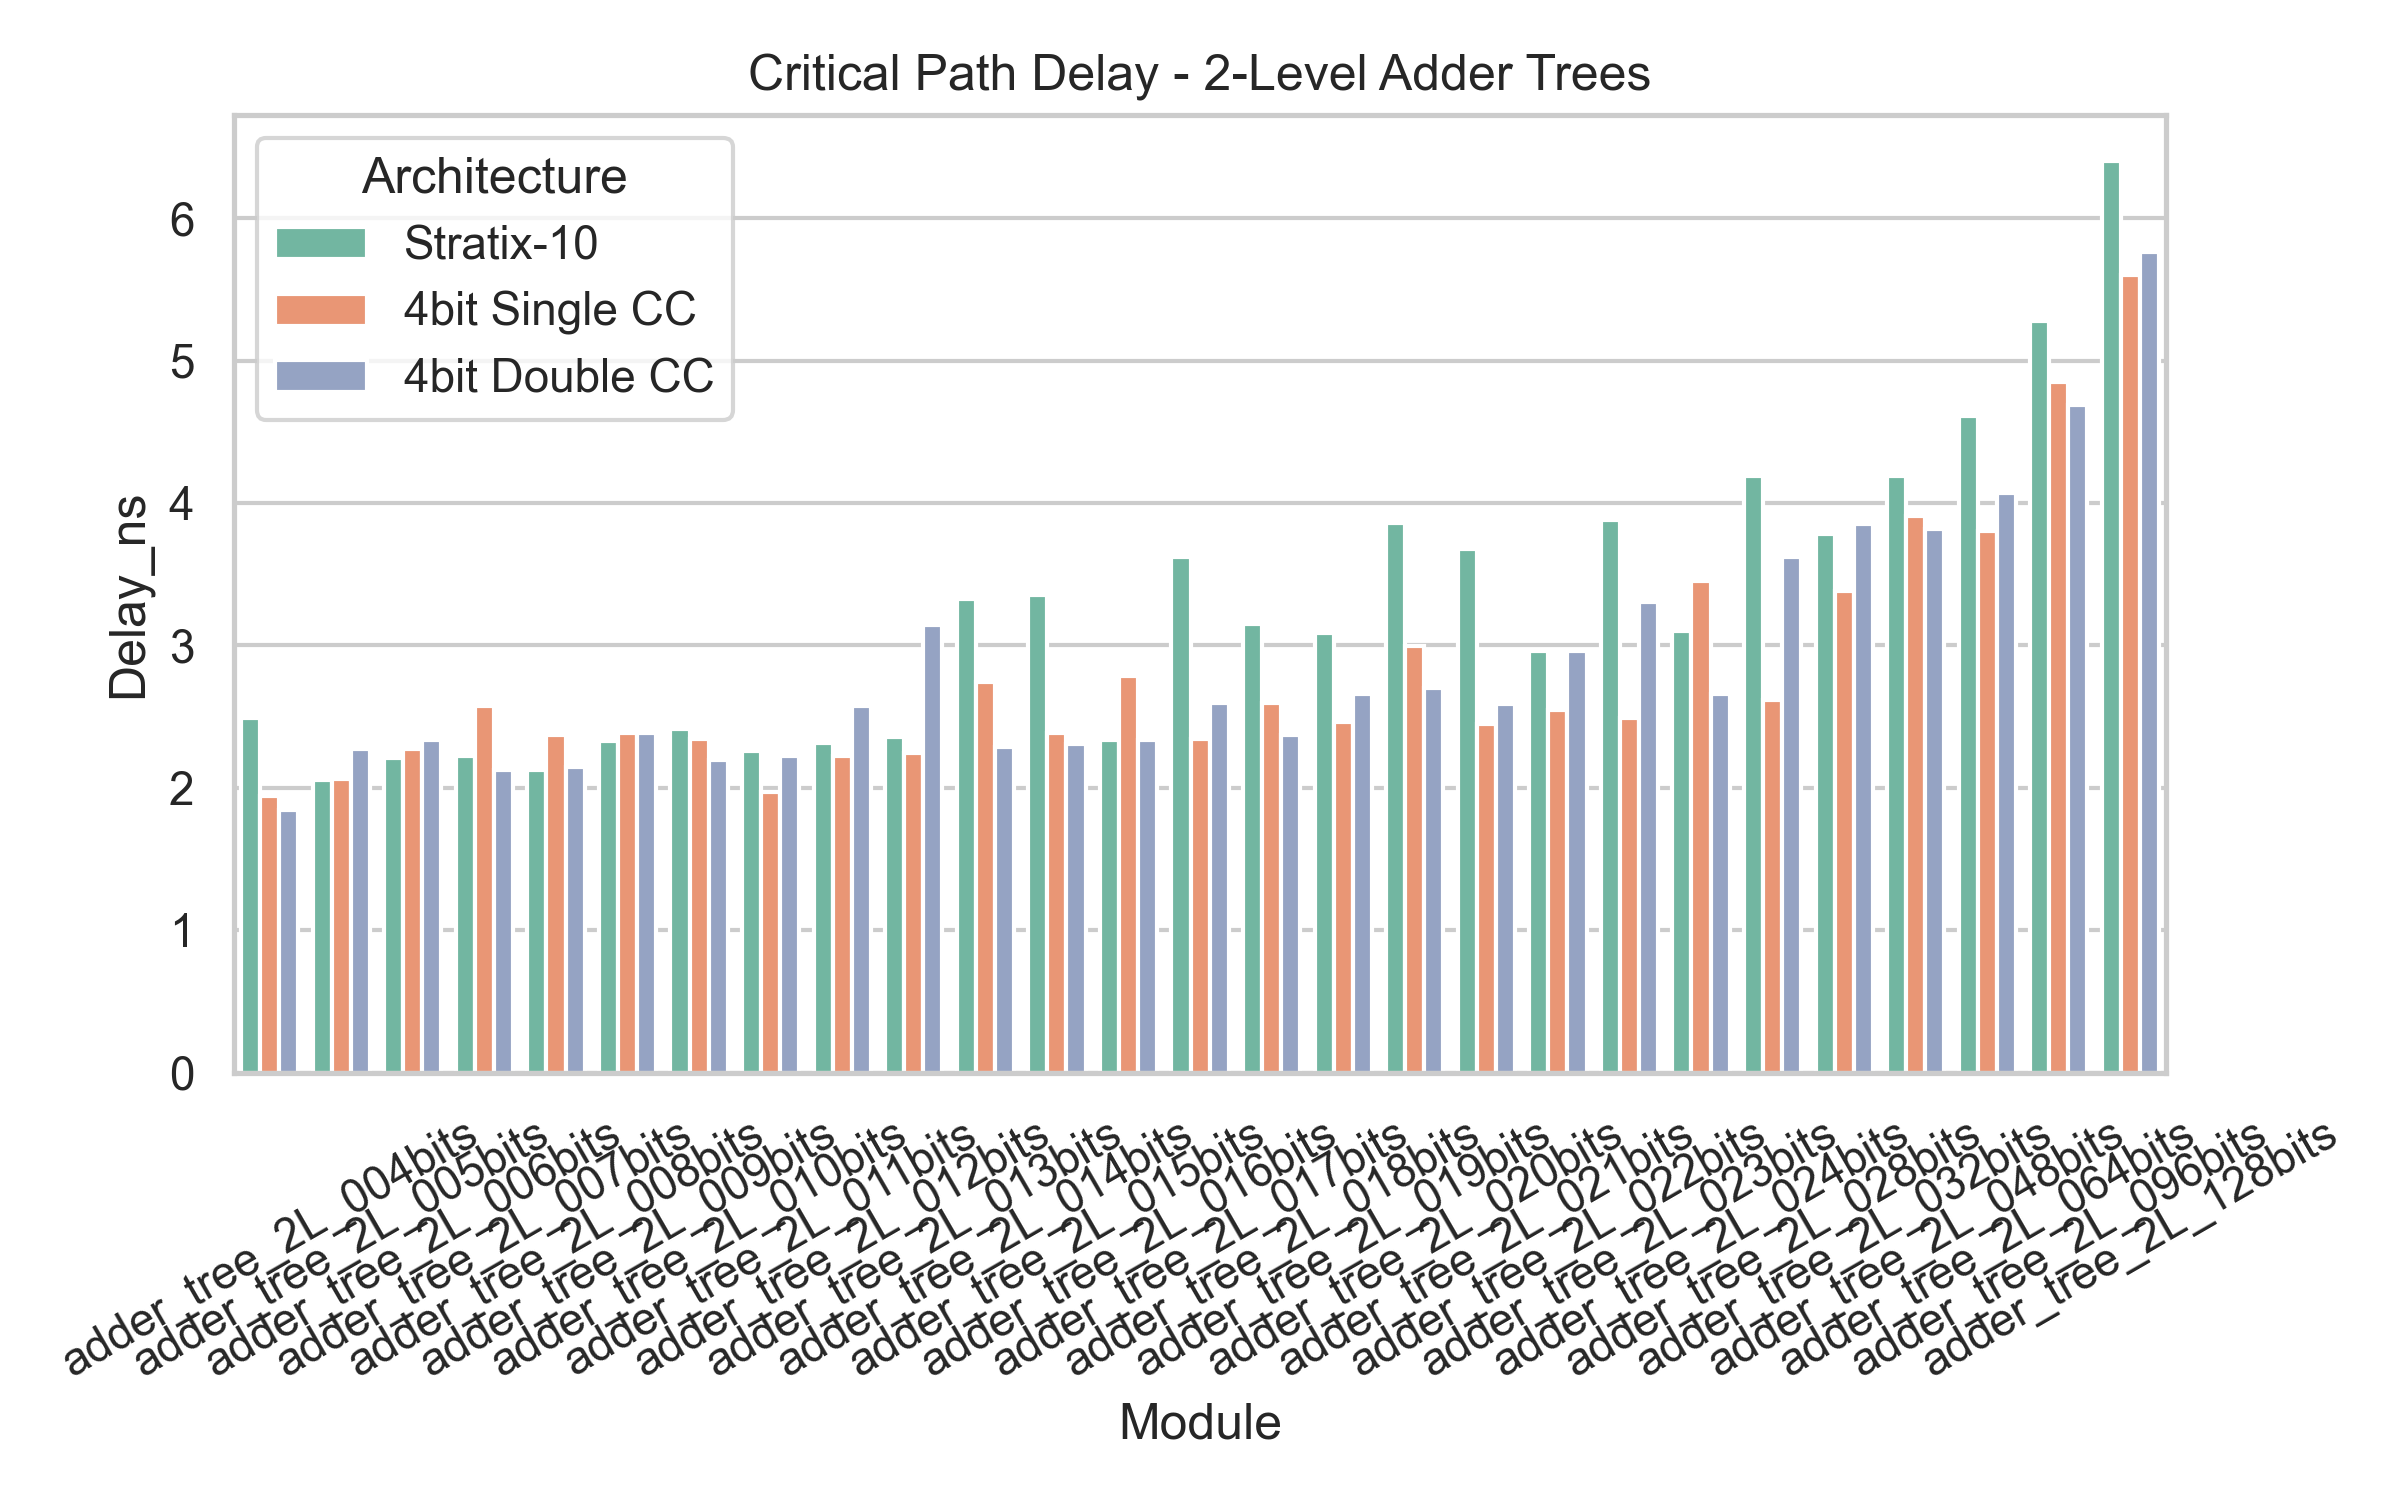
\includegraphics[scale = 0.75]{Figures/adder_trees_2lvl_delay_bar_plt.png}}
	\caption{Critical Path Delays of 2-Level Adder Trees across Bitwidths}
	\label{fig:critical-path-delays-of-2-level-adder-trees-across-bitwidhts}
\end{figure}

For small operand sizes (e.g., 4 to 16 bits), all three architectures show comparable performance, indicating minimal carry chain depth. However, as the operand width grows beyond 64 bits, the benefit of specialized arithmetic routing becomes more apparent, particularly in the Double Carry Chain, which maintains a shallower critical path thanks to its dual-path propagation. This validates the architectural benefit of embedding multiple carry chains in performance-critical datapaths.

\subsection{Area in Adder Trees}
Fig.\ref{fig:Area-(MWTA)-Consumption-of-3-Level-Adder-Trees-across-Architectures} illustrates the area consumption of 3-level adder trees across the three architectures. All architectures show an expected exponential increase in area as operand bit-width increases. However, the difference in area between architectures remains relatively modest for small to mid-sized adders. Notably, the 4-bit Double Carry Chain tends to consume slightly more area than the Single Carry variant, a trade-off resulting from its more complex internal logic structure and wider data paths. Stratix-10, despite being a highly capable general-purpose FPGA, does not show superior area efficiency in this context, suggesting its resources are optimized for broader flexibility rather than arithmetic compactness.

\begin{figure}[H]
	\centerline{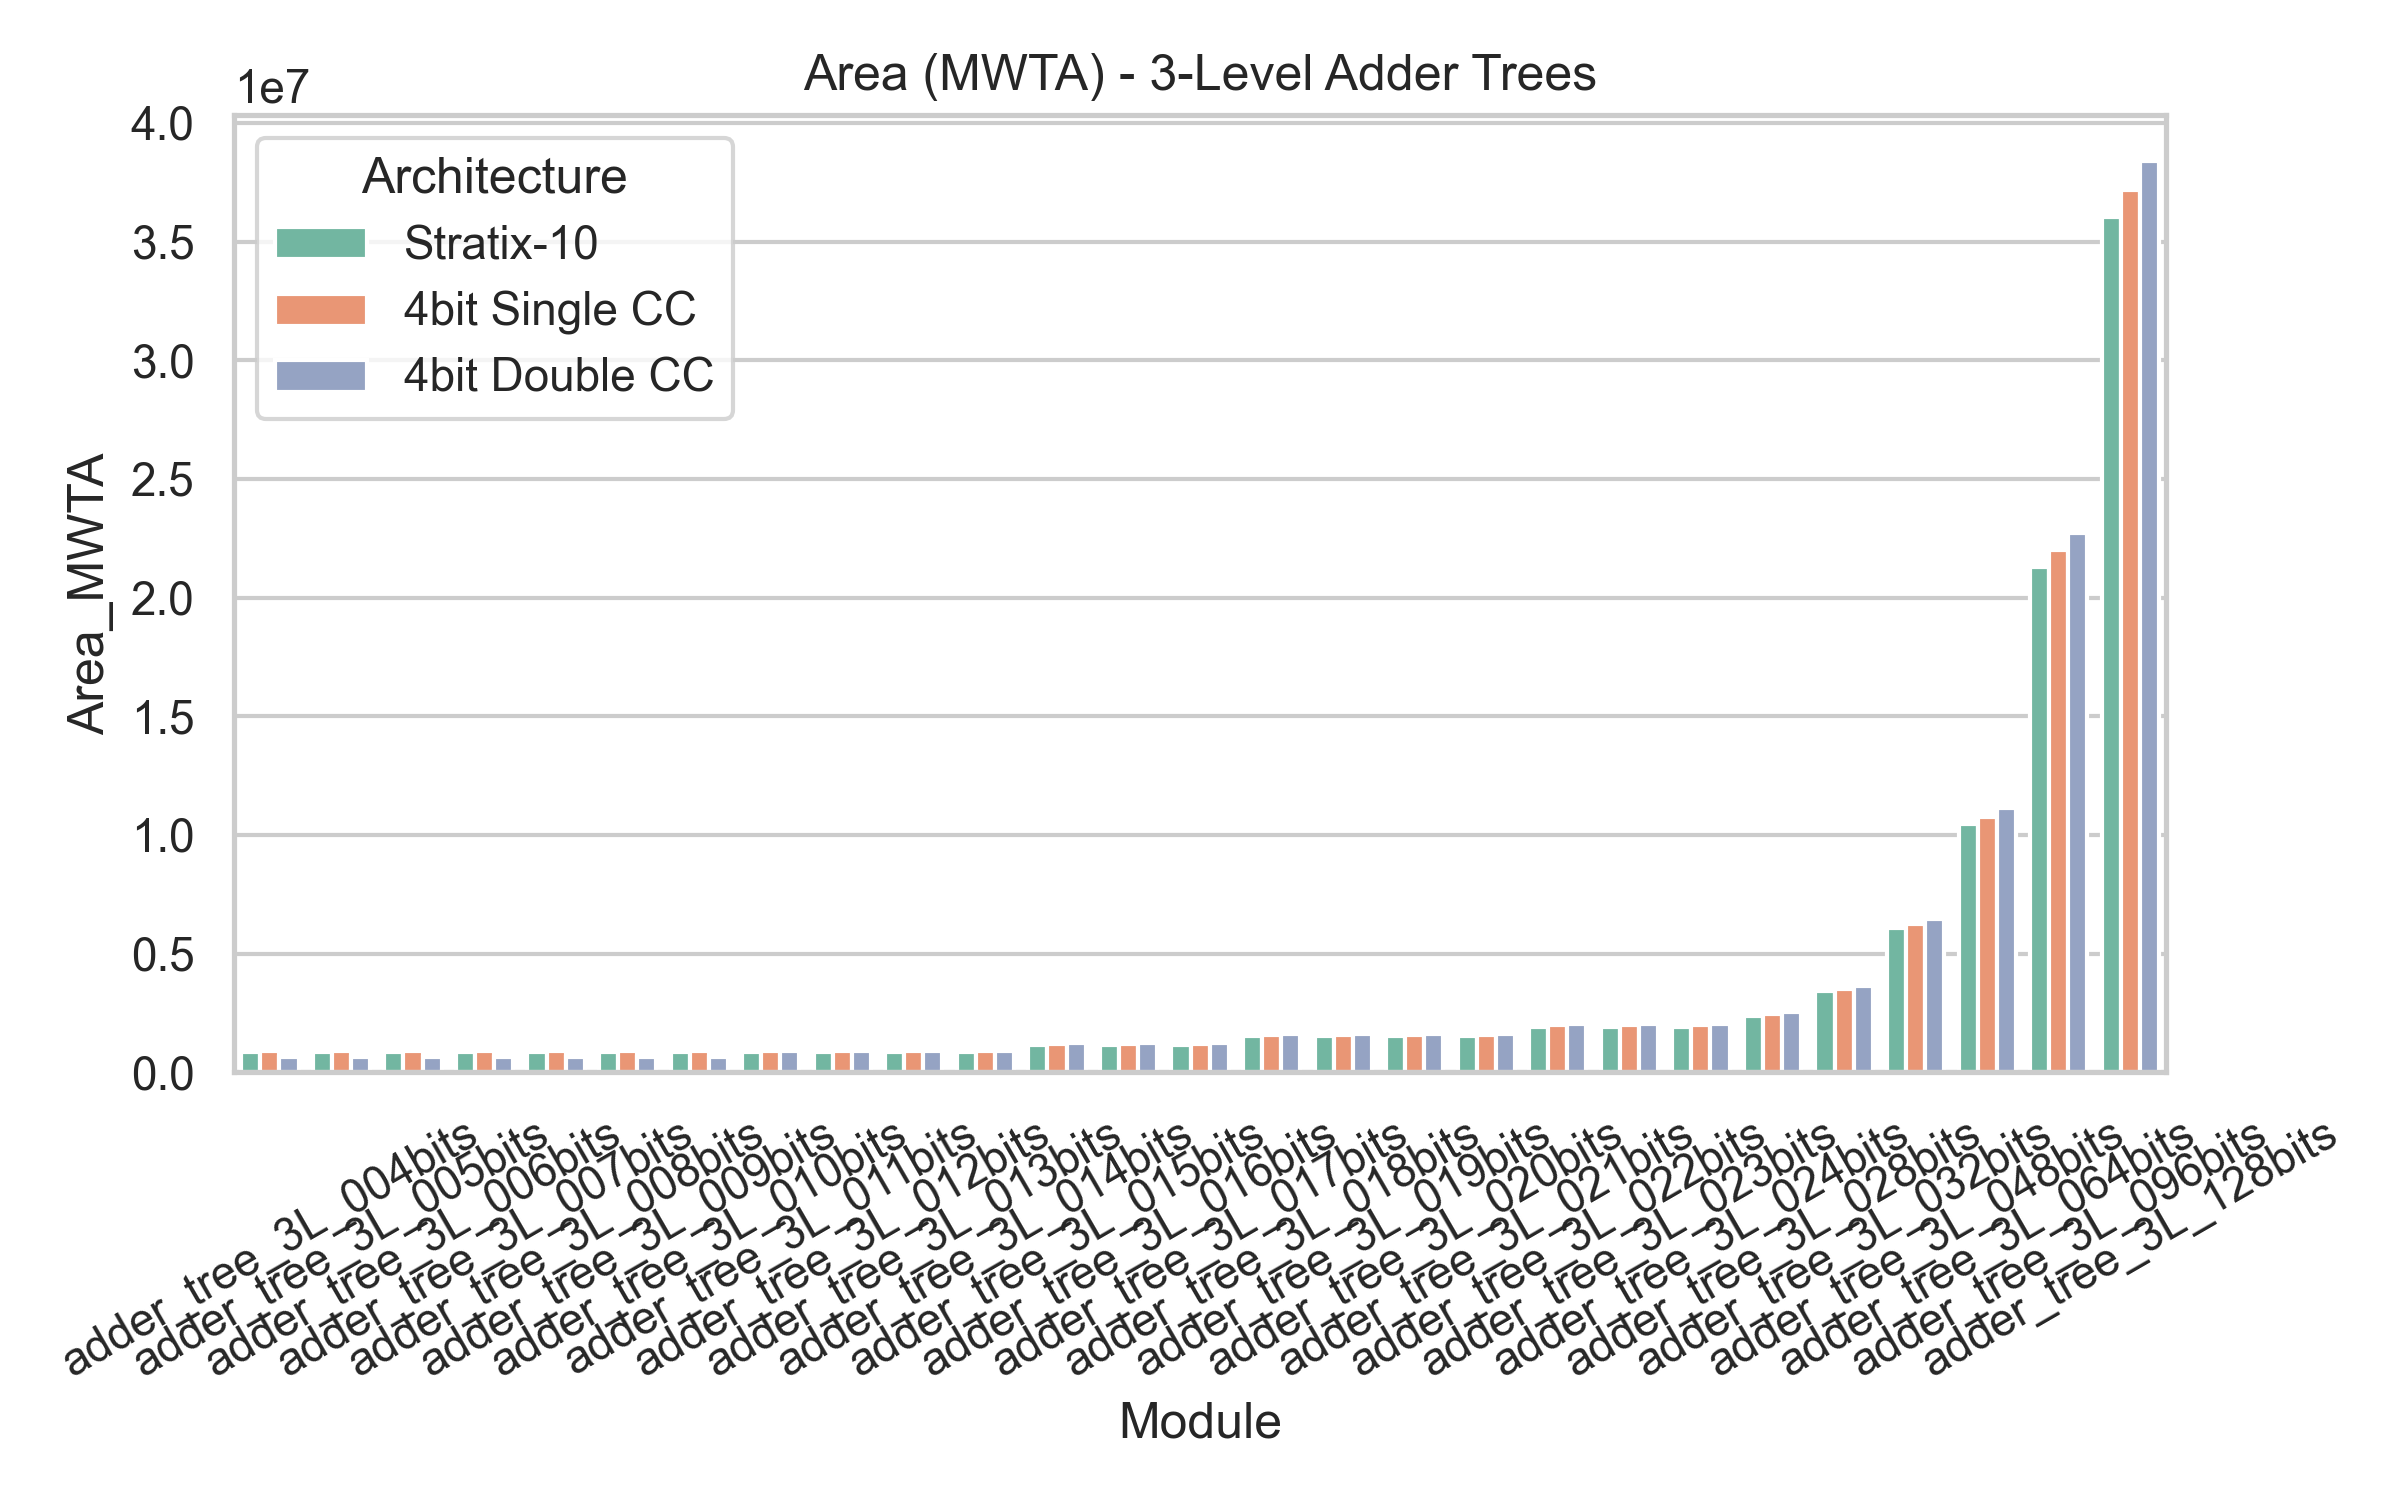
\includegraphics[scale = 0.75]{Figures/adder_trees_3lvl_area_bar_plt.png}}
	\caption{Area (MWTA) Consumption of 3-Level Adder Trees across Architectures}
	\label{fig:Area-(MWTA)-Consumption-of-3-Level-Adder-Trees-across-Architectures}
\end{figure}

This observation reinforces the utility of custom, narrow-precision FPGA fabrics for ML-centric arithmetic workloads, where area efficiency and delay optimization often outweigh the need for generalized functionality.

\subsection{Delay vs Area in FIR Filters}
Fig.\ref{fig:Critical Path Delay vs Area (MWTA) for Wallace Tree based FIR Filters} presents a delay vs area scatter plot for pipelined FIR filters implemented with Wallace Tree multipliers. The data reveals distinct performance clusters for each architecture. In lower-area designs (e.g., filters with fewer taps or lower bit-widths), all three architectures demonstrate similarly low delay (~1–2 ns), indicating minimal routing pressure and simple datapaths. However, as complexity increases, Stratix-10 shows tighter delay control for medium-area FIRs, likely due to its optimized DSP and routing fabric.

\begin{figure}[H]
	\centerline{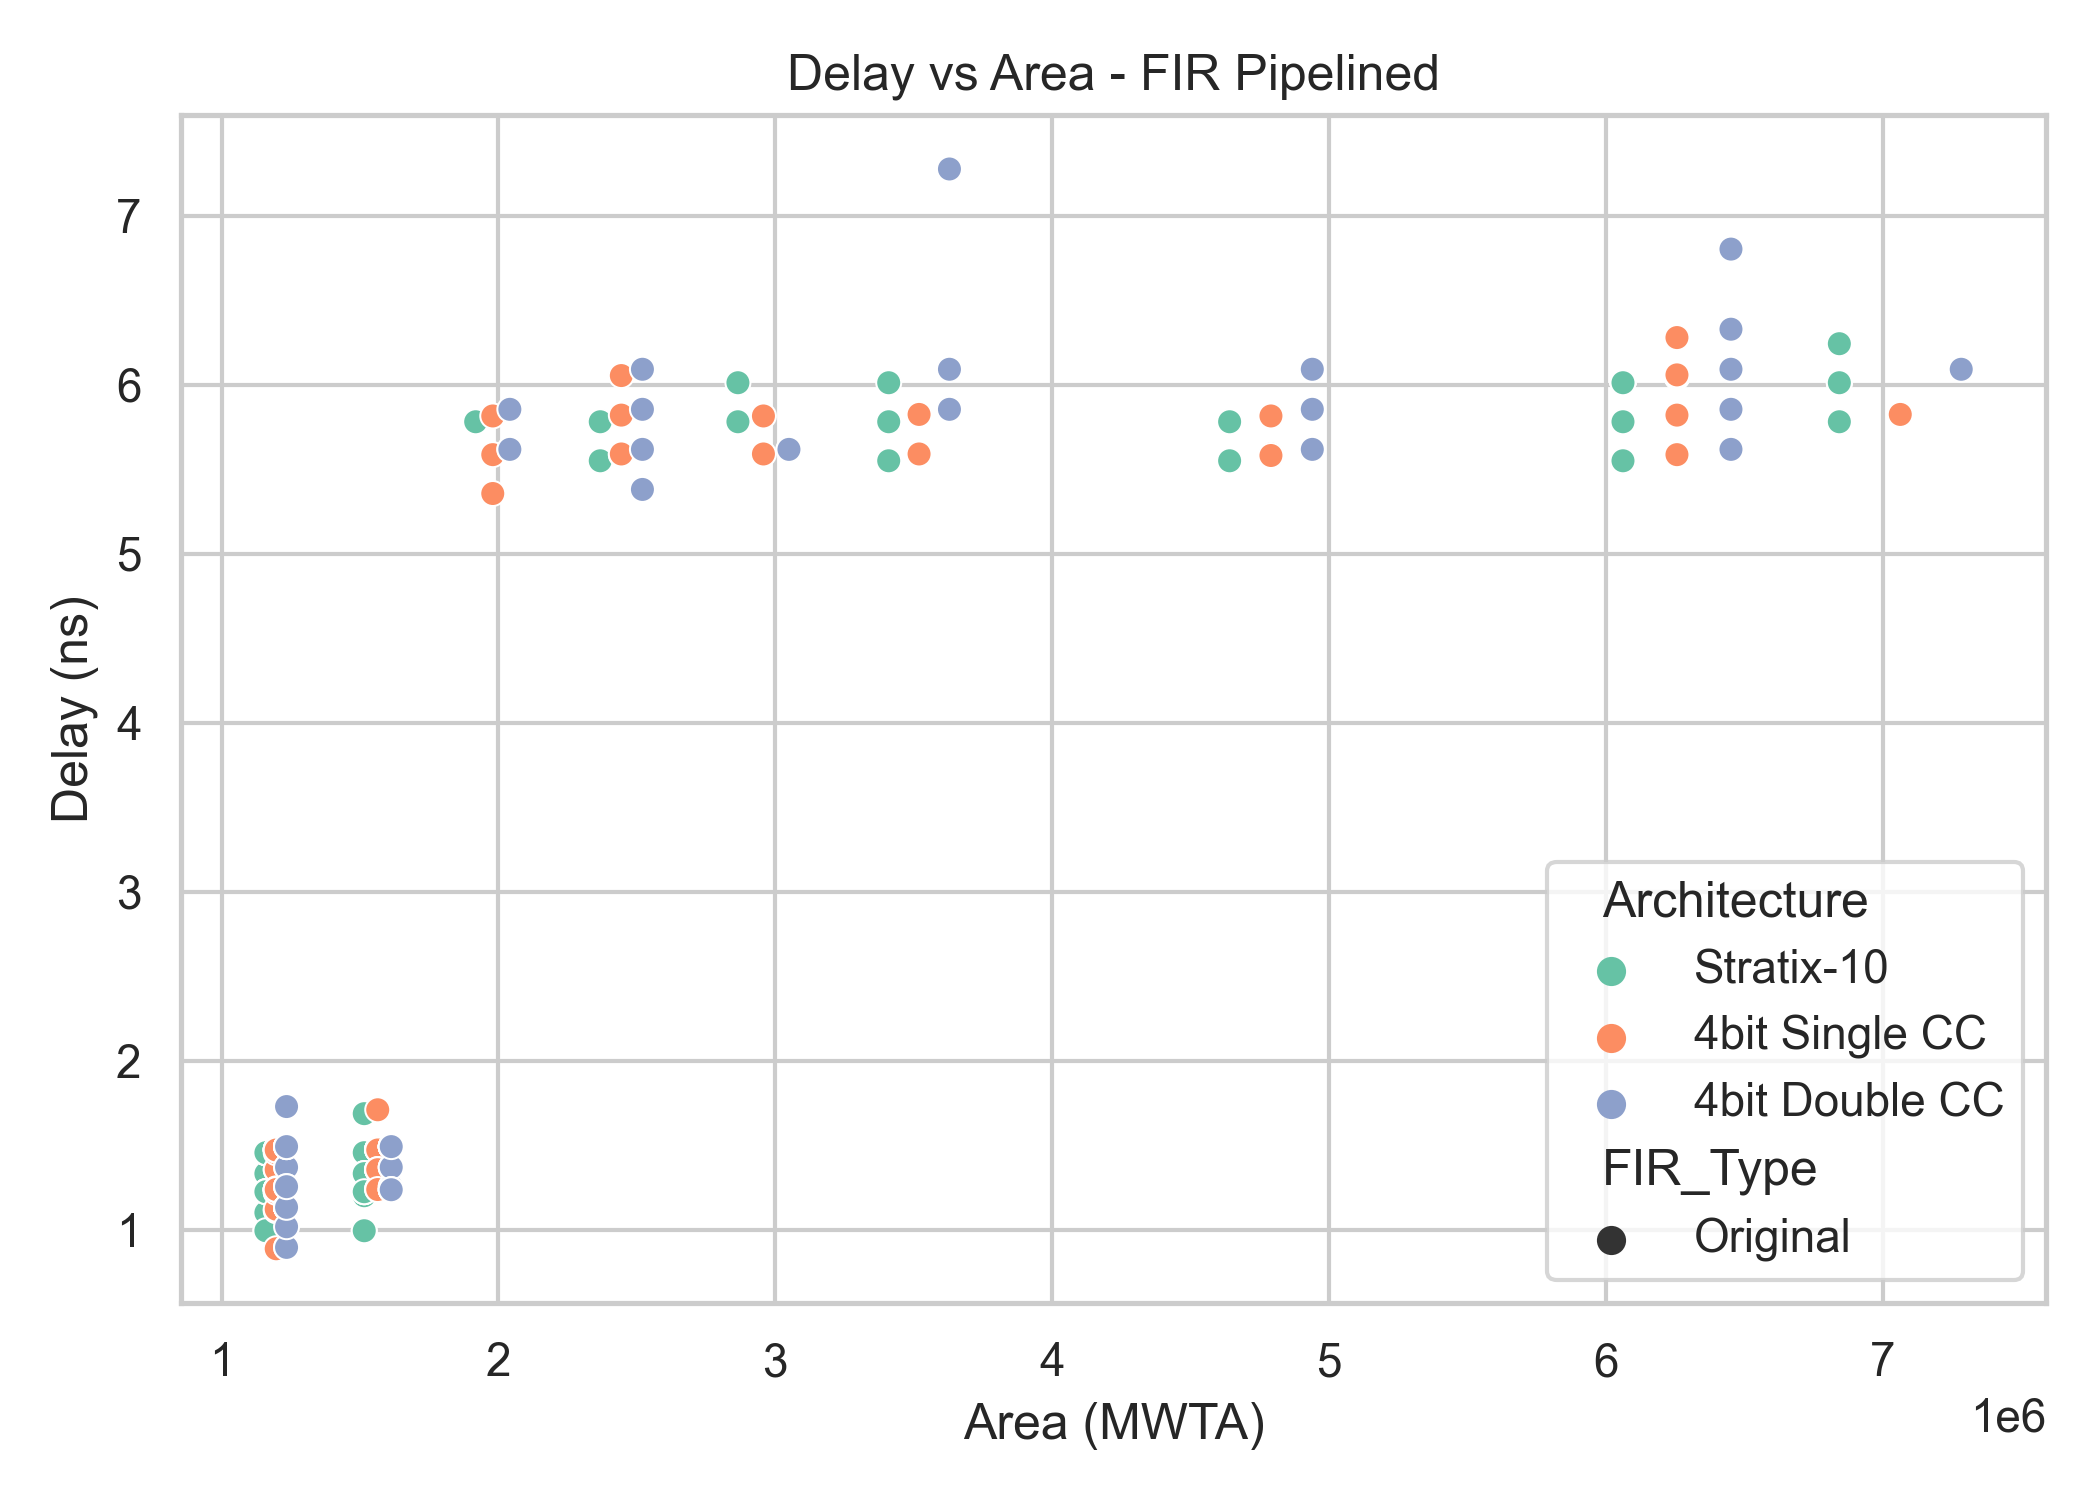
\includegraphics[scale = 0.75]{Figures/fir_pipelined_wallace_delay_area_plt.png}}
	\caption{Critical Path Delay vs Area (MWTA) for Wallace Tree based FIR Filters}
	\label{fig:Critical Path Delay vs Area (MWTA) for Wallace Tree based FIR Filters}
\end{figure}

Interestingly, in larger FIR designs, the 4-bit Single Carry Chain often outperforms Stratix-10 in delay, while maintaining area efficiency. The Double Carry Chain generally uses more area but occasionally yields better delay, reflecting its architectural strength in wide, parallel multiplications. These results demonstrate that specialized carry chain architectures can rival or even surpass commercial FPGAs in delay-area efficiency for structured, low-bitwidth arithmetic pipelines.

\subsection{Delay-Area Product of Unpipelined Wallace Tree based FIR Filters}
The delay-area product analysis of unpipelined FIR filter implementations across three distinct architectures reveals significant performance disparities and scaling characteristics, as shown in Fig.\ref{fig:Delay-Area Product Analysis of Wallace-Tree Unpipelined FIR Filters}.

\begin{figure}[H]
	\centerline{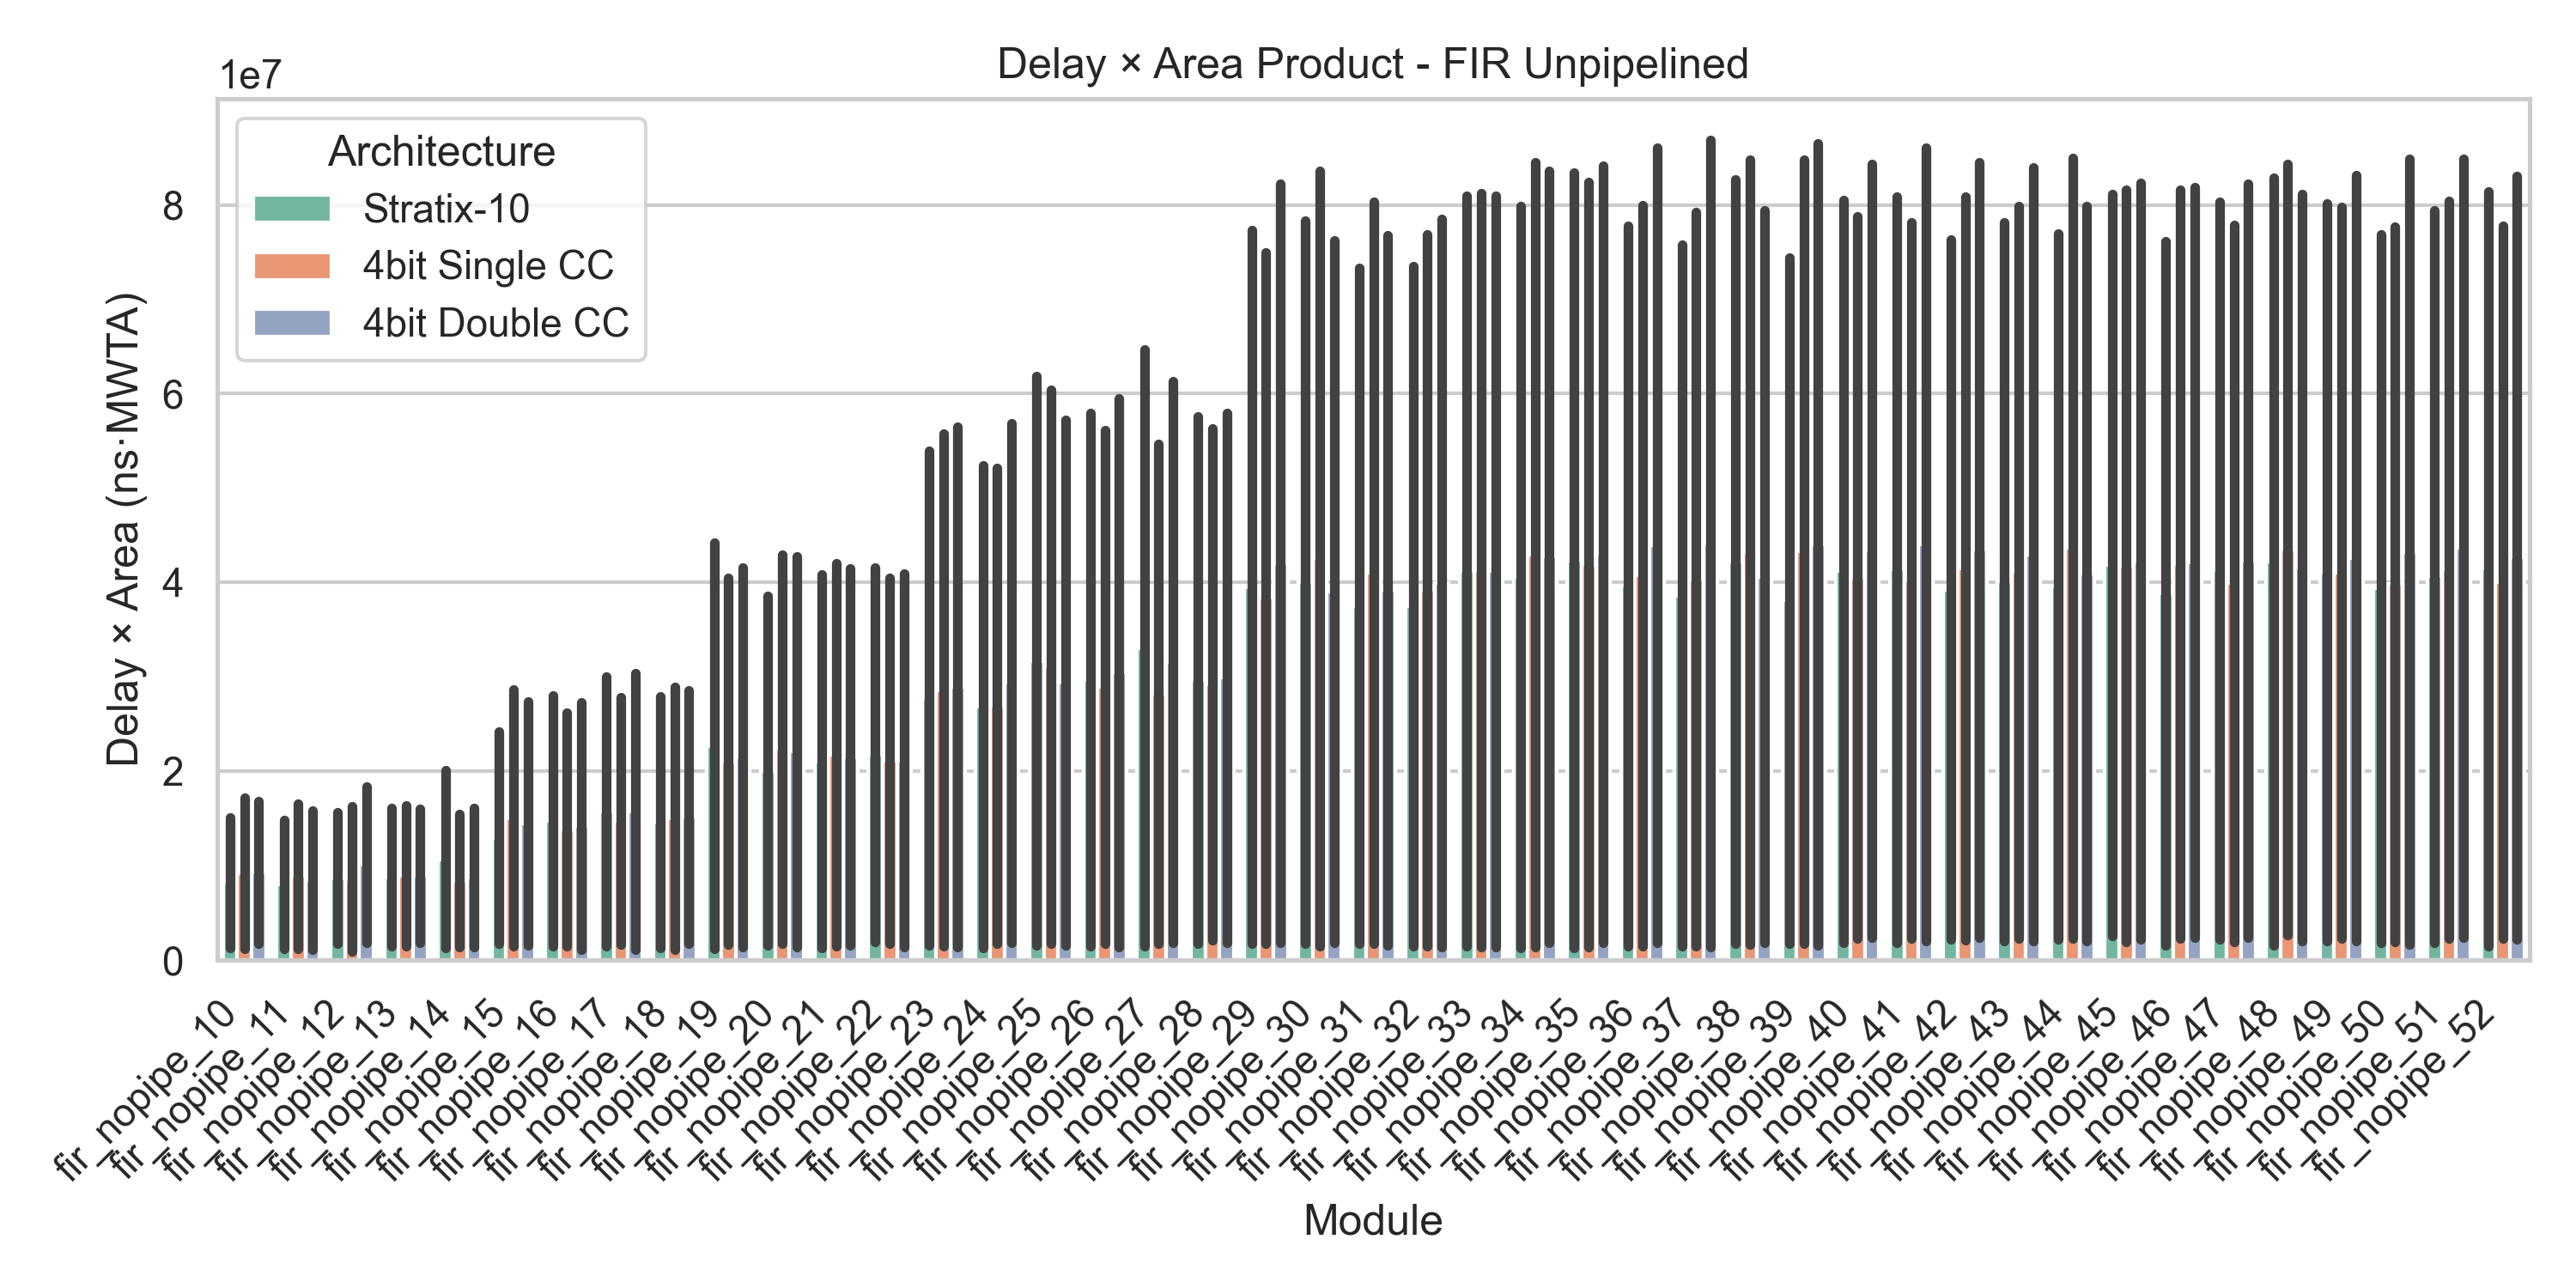
\includegraphics[scale = 0.75]{Figures/fir_unpipelined_wallace_delay_area_prod_plt.png}}
	\caption{Delay-Area Product Analysis of Wallace-Tree Unpipelined FIR Filters}
	\label{fig:Delay-Area Product Analysis of Wallace-Tree Unpipelined FIR Filters}
\end{figure}

The Stratix-10 architecture demonstrates superior efficiency throughout the entire range of filter sizes, consistently achieving the lowest delay-area products with values ranging from approximately 1.5e6 to 8e6 ns·MWTA across modules fir-nopipe-10 through fir-nopipe-52. In contrast, both 4-bit implementations exhibit substantially higher delay-area products, with the 4-bit Single CC architecture showing moderate performance degradation and the 4-bit Double CC architecture displaying the poorest efficiency metrics. All three architectures demonstrate approximately linear scaling behavior with increasing filter complexity, though a notable discontinuity occurs around modules 28-30, suggesting a critical threshold in design complexity. The performance gap between architectures remains relatively constant across different module sizes, with Stratix-10 maintaining approximately 80-90\% lower delay-area products compared to the 4-bit implementations. These results indicate that for unpipelined FIR filter applications, the Stratix-10 FPGA architecture provides substantially better area-delay efficiency, while the 4-bit Double CC approach offers no advantage over the Single CC configuration and should be avoided for this class of implementations.

\subsection{Peak Operational Frequency Analysis}
The top 5 operating frequencies achieved across all benchmarks are summarized in Table 5.1. Notably, the highest frequency — 647.22 MHz — is achieved on the 4-bit Double Carry Chain architecture running a pipelined FIR filter with 12 taps. This aligns with expectations, as the pipelined structure limits combinational depth per stage, while the double carry design accelerates propagation. Interestingly, the 4-bit Single Carry Chain outperforms Stratix-10 in three out of the five cases, demonstrating that targeted low-bitwidth arithmetic architectures can be more frequency-efficient than general-purpose high-end FPGAs in certain domains.

\begin{table}[htb]
	\centering
	\fontsize{10}{12}\selectfont
	\caption{Peak Operational Frequencies}
	\label{tab:peak-operational-frequencies}
	\begin{tabular}{|p{3cm}|c|c|c|}
		%\hline
		%\multicolumn{4}{|c|}{Country List} \\
		\hline
		\textbf{Module}& \textbf {4-Bit Double CC} & \textbf {4-Bit Single CC} & \textbf{Stratix-10}\\
		\hline
		fir-nopipe-11 & 609.25 MHz & 545.15 MHz & 553.98 MHz\\\hline
		fir-pipe-14 & 447.12 MHz & 652.84 MHz & 544.12 MHz\\\hline
		fir-pipe-12 & 647.22 MHz & 489.85 MHz & 494.61 MHz\\\hline
		fir-pipe-27 & 576.59 MHz & 493.45 MHz & 544.12 MHz\\\hline
		fir-pipe-10 & 530.43 MHz & 538.97 MHz & 540.52 MHz\\\hline
		\end{tabular}
\end{table}

These frequency results reinforce the architectural trade-offs: while Stratix-10 offers predictable performance across a wide range of designs, custom carry chain architectures can be tuned to outperform it in narrow, arithmetic-intensive workloads — particularly when pipelining and bit-width optimization are applied.

\section{FPGA Implementation of Manojavam}
This section presents the performance and resource utilization of the Manojavam PCA accelerator when implemented on a Xilinx Artix-7 XC7A35T FPGA using Vivado 2024.1 ML Edition. We report on post-synthesis and post-implementation metrics including logic utilization (LUTs, FFs, DSPs, and BRAMs), maximum achieved clock frequency, power consumption, and timing slack. These results demonstrate how the RTL design maps onto mid-range FPGA fabric, highlighting throughput, energy efficiency, and timing closure for the whole architecture.

\subsection{Resource Consumption}
The FPGA resource utilization of the Manojavam accelerator, synthesized and implemented on the Artix-7 XC7A35T device, is summarized in Table.\ref{tab:manojavam-resource-consumption}.

\begin{table}[htb]
	\centering
	\fontsize{10}{12}\selectfont
	\caption{Manojavam's Resource Consumption}
	\label{tab:manojavam-resource-consumption}
	\begin{tabular}{|p{3cm}|c|c|c|}
		%\hline
		%\multicolumn{4}{|c|}{Country List} \\
		\hline
		\textbf{Resource}& \textbf {Used} & \textbf {Available} & \textbf{Utilization (\%)}\\
		\hline
		LUT & 9796 & 20800 & 47.10\%\\\hline
		FF & 23077 & 41600 & 55.47\%\\\hline
		BRAM & 30.5 & 50 & 61.00\%\\\hline
		DSP & 64 & 90 & 71.11\%\\\hline
	\end{tabular}
\end{table}

This resource profile reflects the architectural demands of Manojavam, which integrates multiple compute-intensive and memory-aware subsystems. The LUT and flip-flop usage—at approximately 47\% and 55\%, respectively—indicates balanced deployment of logic resources, with sufficient margin available for further modular expansion or integration of debugging logic.

BRAM consumption is moderately high at 61\%, consistent with the design’s use of L1 private and shared caches, staging buffers, and operand tile storage for block streaming. This level of memory usage validates the effectiveness of the memory hierarchy and suggests that the accelerator makes full use of the available on-chip memory without exhausting it.

The most saturated resource is the DSP slice count, with 71.11\% of the available multipliers in use. This is directly attributed to the matrix multiplication engine and its 8 systolic arrays, each employing DSP-based MAC units for dense arithmetic. The relatively high DSP usage is a strong indicator that the design is compute-dense and optimized for throughput, making full use of the device's parallel arithmetic capabilities.

In summary, Manojavam fits comfortably within the Artix-7 fabric, striking a balance between compute intensity and architectural scalability. The current resource utilization confirms that the design remains extensible while still exercising the FPGA in a realistic deployment scenario.

\subsection{Power Consumption}
The total power consumption of the Manojavam accelerator on the Artix-7 XC7A35T FPGA is measured at 1.271 W, with the power breakdown across various subsystems detailed below:

\begin{table}[htb]
	\centering
	\fontsize{10}{12}\selectfont
	\caption{Manojavam's Power Consumption}
	\label{tab:manojavam-power-consumption}
	\begin{tabular}{|p{3cm}|c|c|}
		%\hline
		%\multicolumn{4}{|c|}{Country List} \\
		\hline
		\textbf{Power Domain}& \textbf {Power (W)} & \textbf {Percentage of Power}\\
		\hline
		Clocks & 0.036 & 2.83\%\\\hline
		Signals & 0.051 & 4.01\%\\\hline
		Logic & 0.037 & 2.91\%\\\hline
		BRAM & 0.001 & 0.08\%\\\hline
		DSP & 0.036 & 2.83\%\\\hline
		I/O & 1.034 & 81.37\%\\\hline
		Total & 1.271 & 100\%\\\hline
	\end{tabular}
\end{table}

The power profile reveals that I/O activity dominates overall power dissipation, accounting for over 81\% of total power. This is expected, as the design involves continuous tile streaming and operand transfers between the host and the accelerator through external interfaces. Such communication-intensive behavior is inherent to block-streaming architectures, especially when external data sources and sinks are involved.

The internal logic, clocking network, and DSP slices each consume less than 3\% of total power, which highlights the energy efficiency of the compute core. Notably, the DSP slice power (0.036 W) is remarkably low considering that 71\% of DSPs are active, suggesting that the systolic MAC units are operating with low switching activity or short critical paths—benefiting from pipelined execution and localized operand reuse.

Memory power (BRAM) is almost negligible at 0.001 W, which indicates that the cache hierarchy is well-localized and not incurring excessive access toggling. This aligns with the design’s emphasis on temporal locality, where operand tiles are reused before being written back, minimizing memory energy per operation.

The low dynamic power across logic, signal, and clock networks further reinforces that the architecture is streamlined and well-pipelined, with minimal unnecessary toggling. Overall, these figures demonstrate that Manojavam is compute-efficient and memory-efficient, with the majority of power attributed to I/O, which could be optimized in future iterations through embedded memory, DMA interfaces, or tighter system integration.

In summary, Manojavam exhibits a high-performance yet power-conscious architecture, where internal compute blocks operate with minimal overhead, and the primary power bottleneck stems from external communication—an expected but optimizable characteristic in FPGA deployments.

\subsection{Timing Report and Summaries}
The FPGA implementation of Manojavam achieved a maximum operational frequency of 200 MHz after placement and routing on the Artix-7 XC7A35T FPGA. This clock rate reflects the ability of the design to maintain high-throughput performance while satisfying strict timing constraints across the datapath, control, and memory subsystems.

The post-implementation timing analysis yielded the following key results, displayed in Table.\ref{tab:manojavam-timing-report}.

\begin{table}[htb]
	\centering
	\fontsize{10}{12}\selectfont
	\caption{Manojavam's Timing Report}
	\label{tab:manojavam-timing-report}
	\begin{tabular}{|p{3cm}|c|}
		%\hline
		%\multicolumn{4}{|c|}{Country List} \\
		\hline
		\textbf{Timing Metric}& \textbf {Value}\\
		\hline
		Operational Frequency & 200 MHz\\\hline
		Worst Negative Slack (WNS) & 0.203 ns\\\hline
		Worst Hold Slack (WHS) & 0.105 ns\\\hline
		Worst Pulse Width Slack (WPWS) & 1.250 ns\\\hline
	\end{tabular}
\end{table} 

The Worst Negative Slack (WNS) of 0.203 ns indicates that the critical paths in the design meet timing with a narrow but acceptable margin. This confirms that the design is operating within the safe frequency envelope dictated by its longest combinational delay paths. The Worst Hold Slack of 0.105 ns also confirms that short-path timing constraints are met, preventing hold violations and ensuring reliable data transfer between pipeline stages.

A Worst Pulse Width Slack of 1.250 ns further validates that clock signals maintain proper pulse widths, ensuring stable triggering of sequential elements throughout the design. These results, taken together, demonstrate that the Manojavam accelerator closes timing at 200 MHz, with headroom to account for minor PVT (process, voltage, temperature) variations.

The ability to achieve this clock rate on a mid-range FPGA, while also supporting a complex systolic matrix engine and hierarchical memory system, highlights the architectural regularity and timing-friendly layout of the design.

\subsection{Accelerator Floorplanning}
The physical floorplanning of Manojavam on the Artix-7 FPGA played a critical role in achieving its high operational frequency and low power consumption. All major subsystems of the accelerator—namely the 8 systolic arrays, cache hierarchy, controller hierarchy, and the Jacobian unit—were carefully positioned in proximity to the modules they interact with most heavily. This strategic placement minimized routing congestion and reduced signal delays across high-activity interconnects.

The floorplan was not left to automatic placement alone; instead, manual partitioning and logic grouping were applied to tightly cluster compute and memory blocks, enabling highly localized data movement. For instance, each systolic array was physically adjacent to its associated private cache and accumulator, while the shared LHS cache was placed centrally for low-latency broadcasting. This layout was instrumental in supporting efficient pipelined streaming, fast operand reuse, and precise timing closure across the entire design.

To the best of our knowledge, Manojavam is the first PCA accelerator to be floorplanned and deployed with such architectural precision, especially on a mid-range FPGA. This meticulous approach directly contributed to the accelerator’s 200 MHz operational frequency and 1.2 W power envelope—metrics that outperform prior art, which often suffer from thermal bottlenecks or timing failure due to unoptimized physical layouts.

\begin{figure}[H]
	\centerline{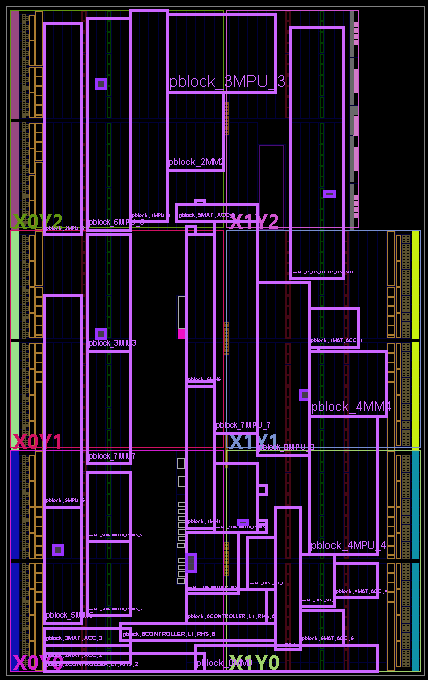
\includegraphics[scale = 1]{Figures/fpga_floorplaned.png}}
	\caption{FPGA Floorplanning of Manojavam}
	\label{fig:FPGA Floorplanning of Manojavam}
\end{figure}

The floorplan layout, shown in Fig.\ref{fig:FPGA Floorplanning of Manojavam}, visually demonstrates the regularity and modularity of the accelerator, further validating the architectural clarity and physical design discipline of the Manojavam system.

\subsection{Comparative Runtime Analysis of PCA on CPU, GPU, and Manojavam Accelerator}
To evaluate the practical benefits of Manojavam in a real-world PCA pipeline, synthetic datasets of dimension $1000xD$, where $D \in {4, 8, 16, 32, 64, 128, 256, 512, 1024}$, were generated using Python. Each dataset was processed through two key stages of the PCA pipeline: matrix multiplication (MM) to compute the covariance matrix, and singular value decomposition (SVD) for eigendecomposition. Execution time for both stages was recorded over 30 independent trials for three platforms:
\begin{enumerate}
	\item CPU : Intel Core i7\cite{chap5-1}
	\item Nvidia A100 (Ampere Architecture)\cite{chap5-2}
	\item Manojavam Accelerator
\end{enumerate}

The average runtime of each stage was recorded, and the total PCA runtime (MM + SVD) was computed. Results were visualized using line plots on logarithmic x-scales to highlight trends across increasing dimensionality.

\subsubsection{Matrix Multiplication (MM) Comparison}
In the MM runtime plot, as shown in Fig.\ref{fig:Execution Time Analysis for Matrix Multiplication}, the Manojavam accelerator shows a consistent linear increase as the feature dimensionality grows, which appears as a straight upward-sloping line on the log-scale graph. This is expected given the tiled 4×4 matrix multiplication strategy with fixed hardware resources and streaming operands. In contrast, both CPU and GPU exhibit nearly flat trends, indicating negligible increases in runtime even as dimensions grow.

\begin{figure}[H]
	\centerline{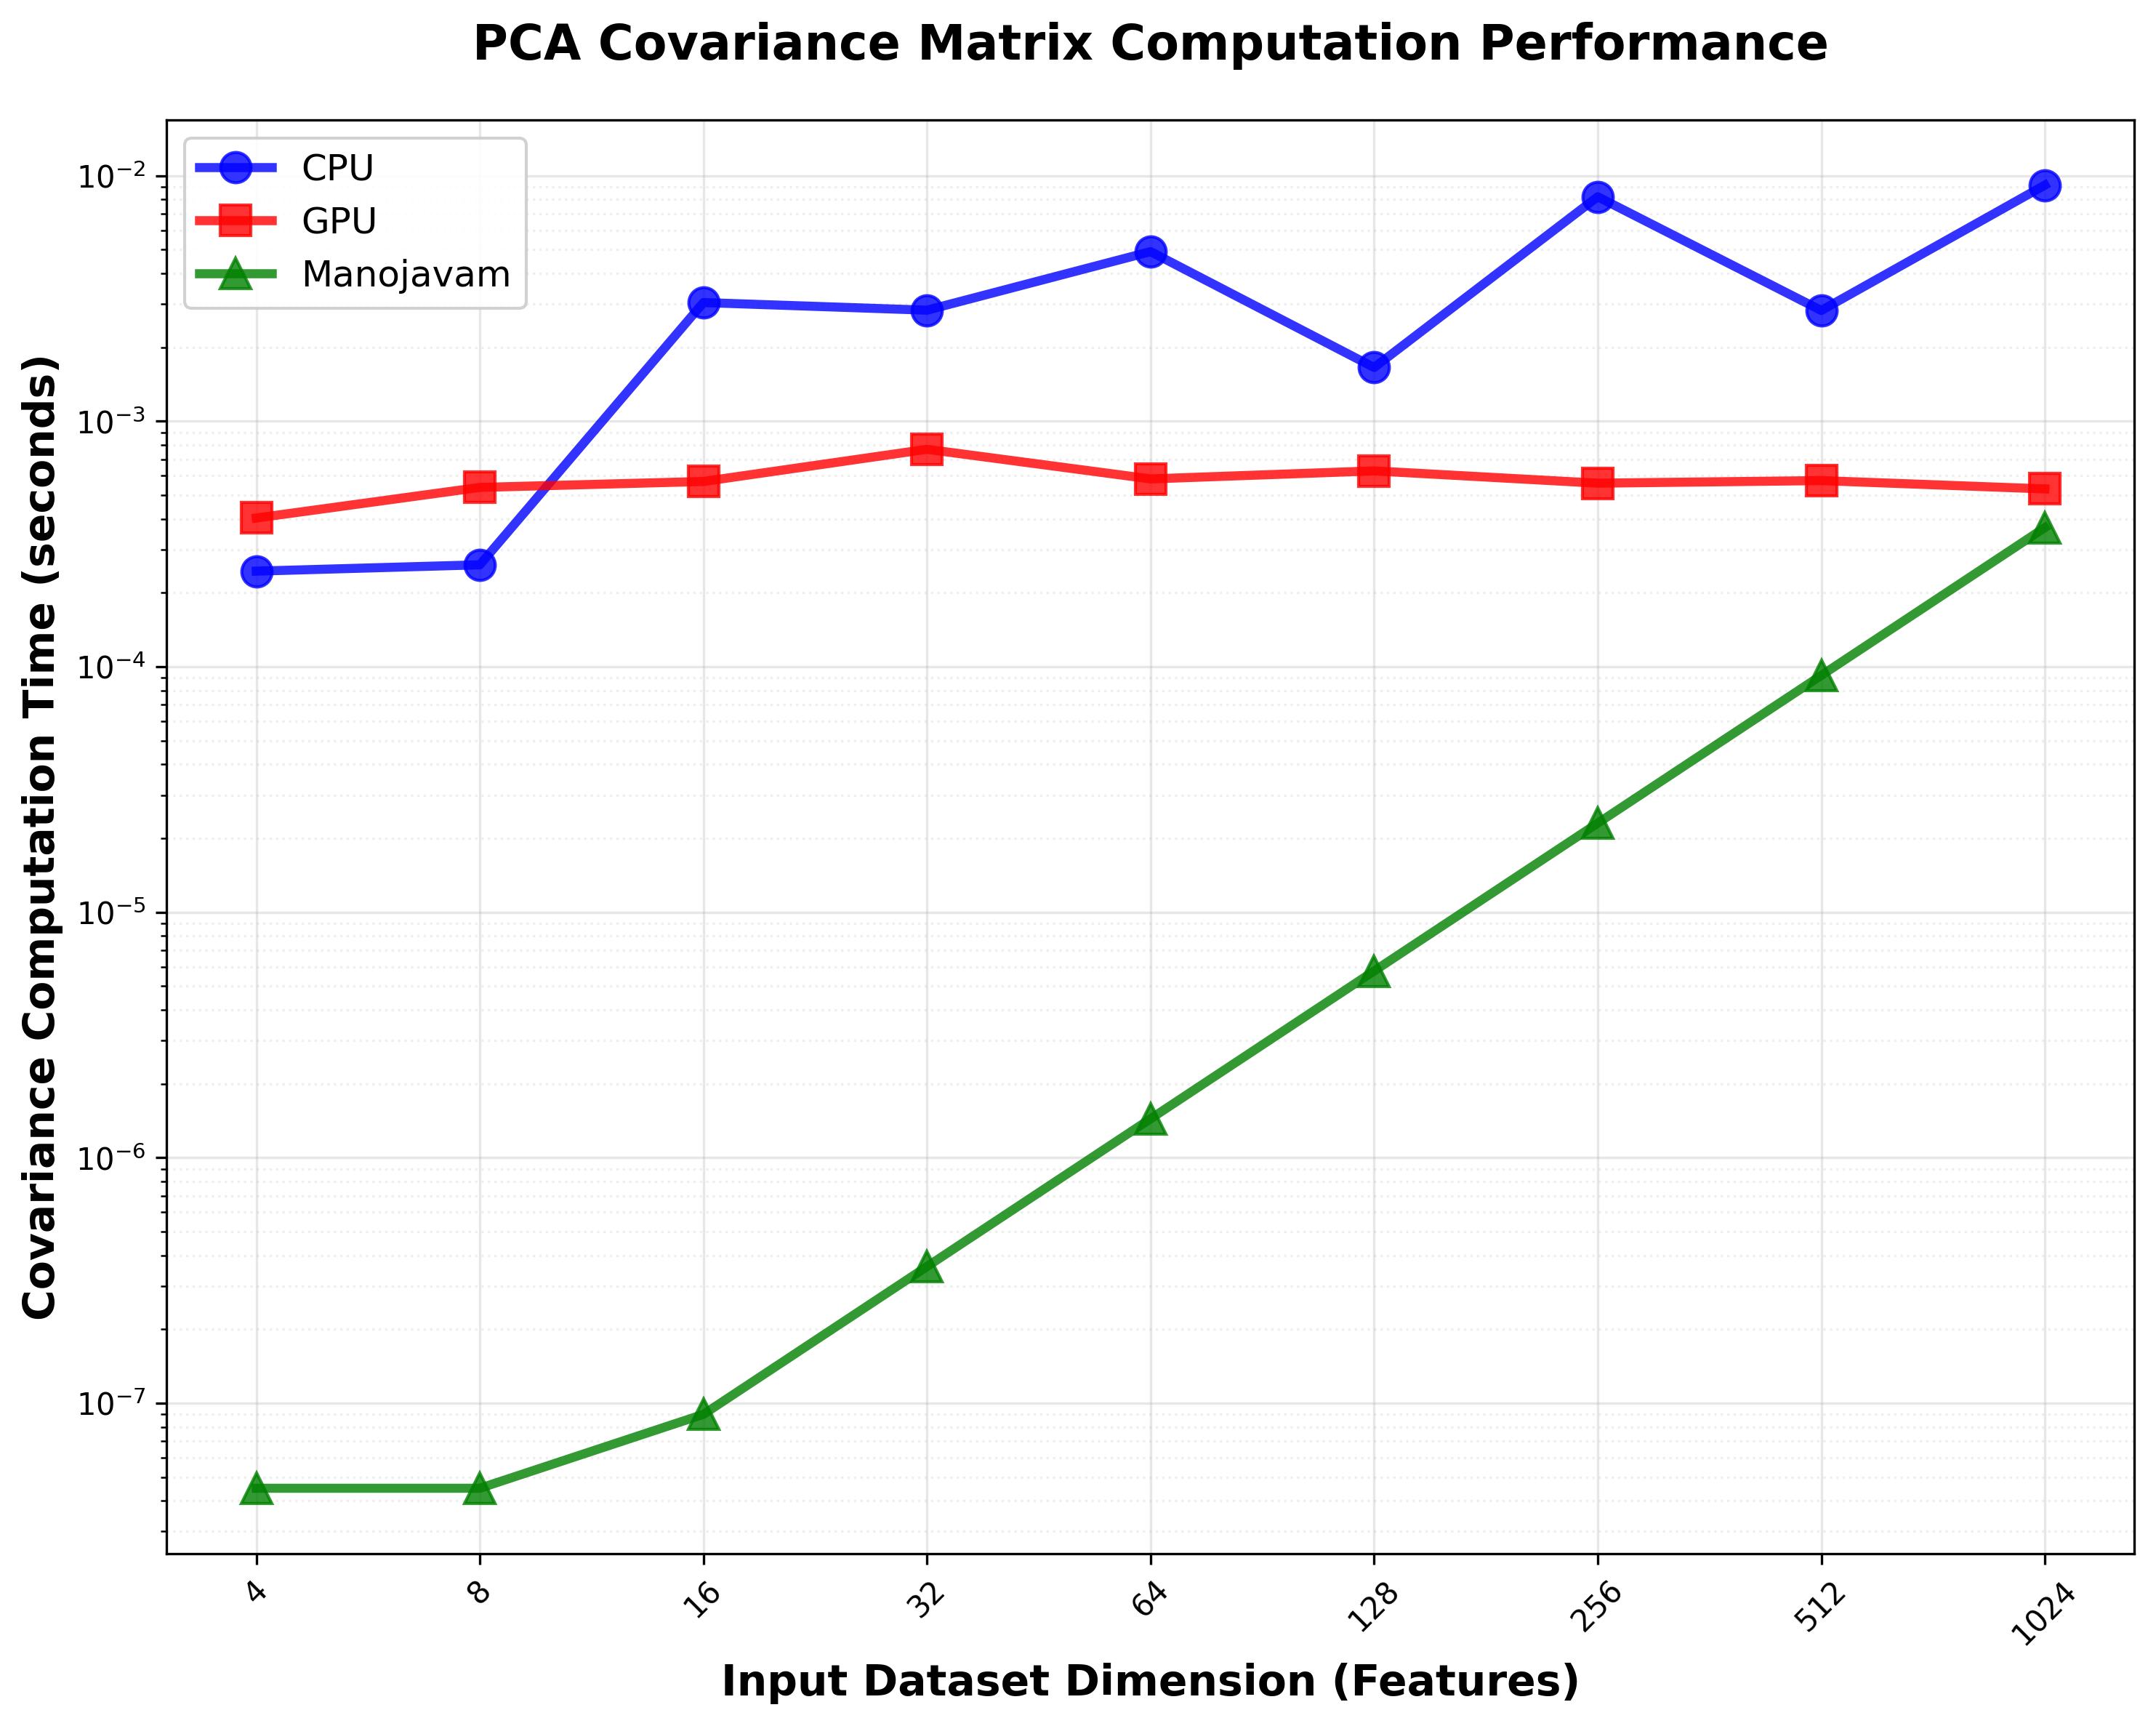
\includegraphics[scale = 0.50]{Figures/covariance_performance.png}}
	\caption{Execution Time Analysis for Matrix Multiplication}
	\label{fig:Execution Time Analysis for Matrix Multiplication}
\end{figure}

This flat trend is due to the use of highly optimized BLAS-backed matrix multiplication libraries (e.g., NumPy on MKL for CPU and cuBLAS for GPU), which leverage massive parallelism, hardware-level acceleration, and cache reuse. While Manojavam does not outperform the CPU or GPU in raw MM runtime, the predictable scaling behavior of its MM engine reflects hardware-deterministic execution, useful in real-time or bounded-latency systems.

\subsubsection{Singular Value Decomposition (SVD) Comparison}
In the SVD runtime plot, all three platforms show linear growth trends with dimensionality, indicating similar algorithmic complexity. However, the Manojavam accelerator consistently achieves the lowest SVD runtime, followed by the GPU, and then the CPU. This ordering holds across all dataset sizes.

\begin{figure}[H]
	\centerline{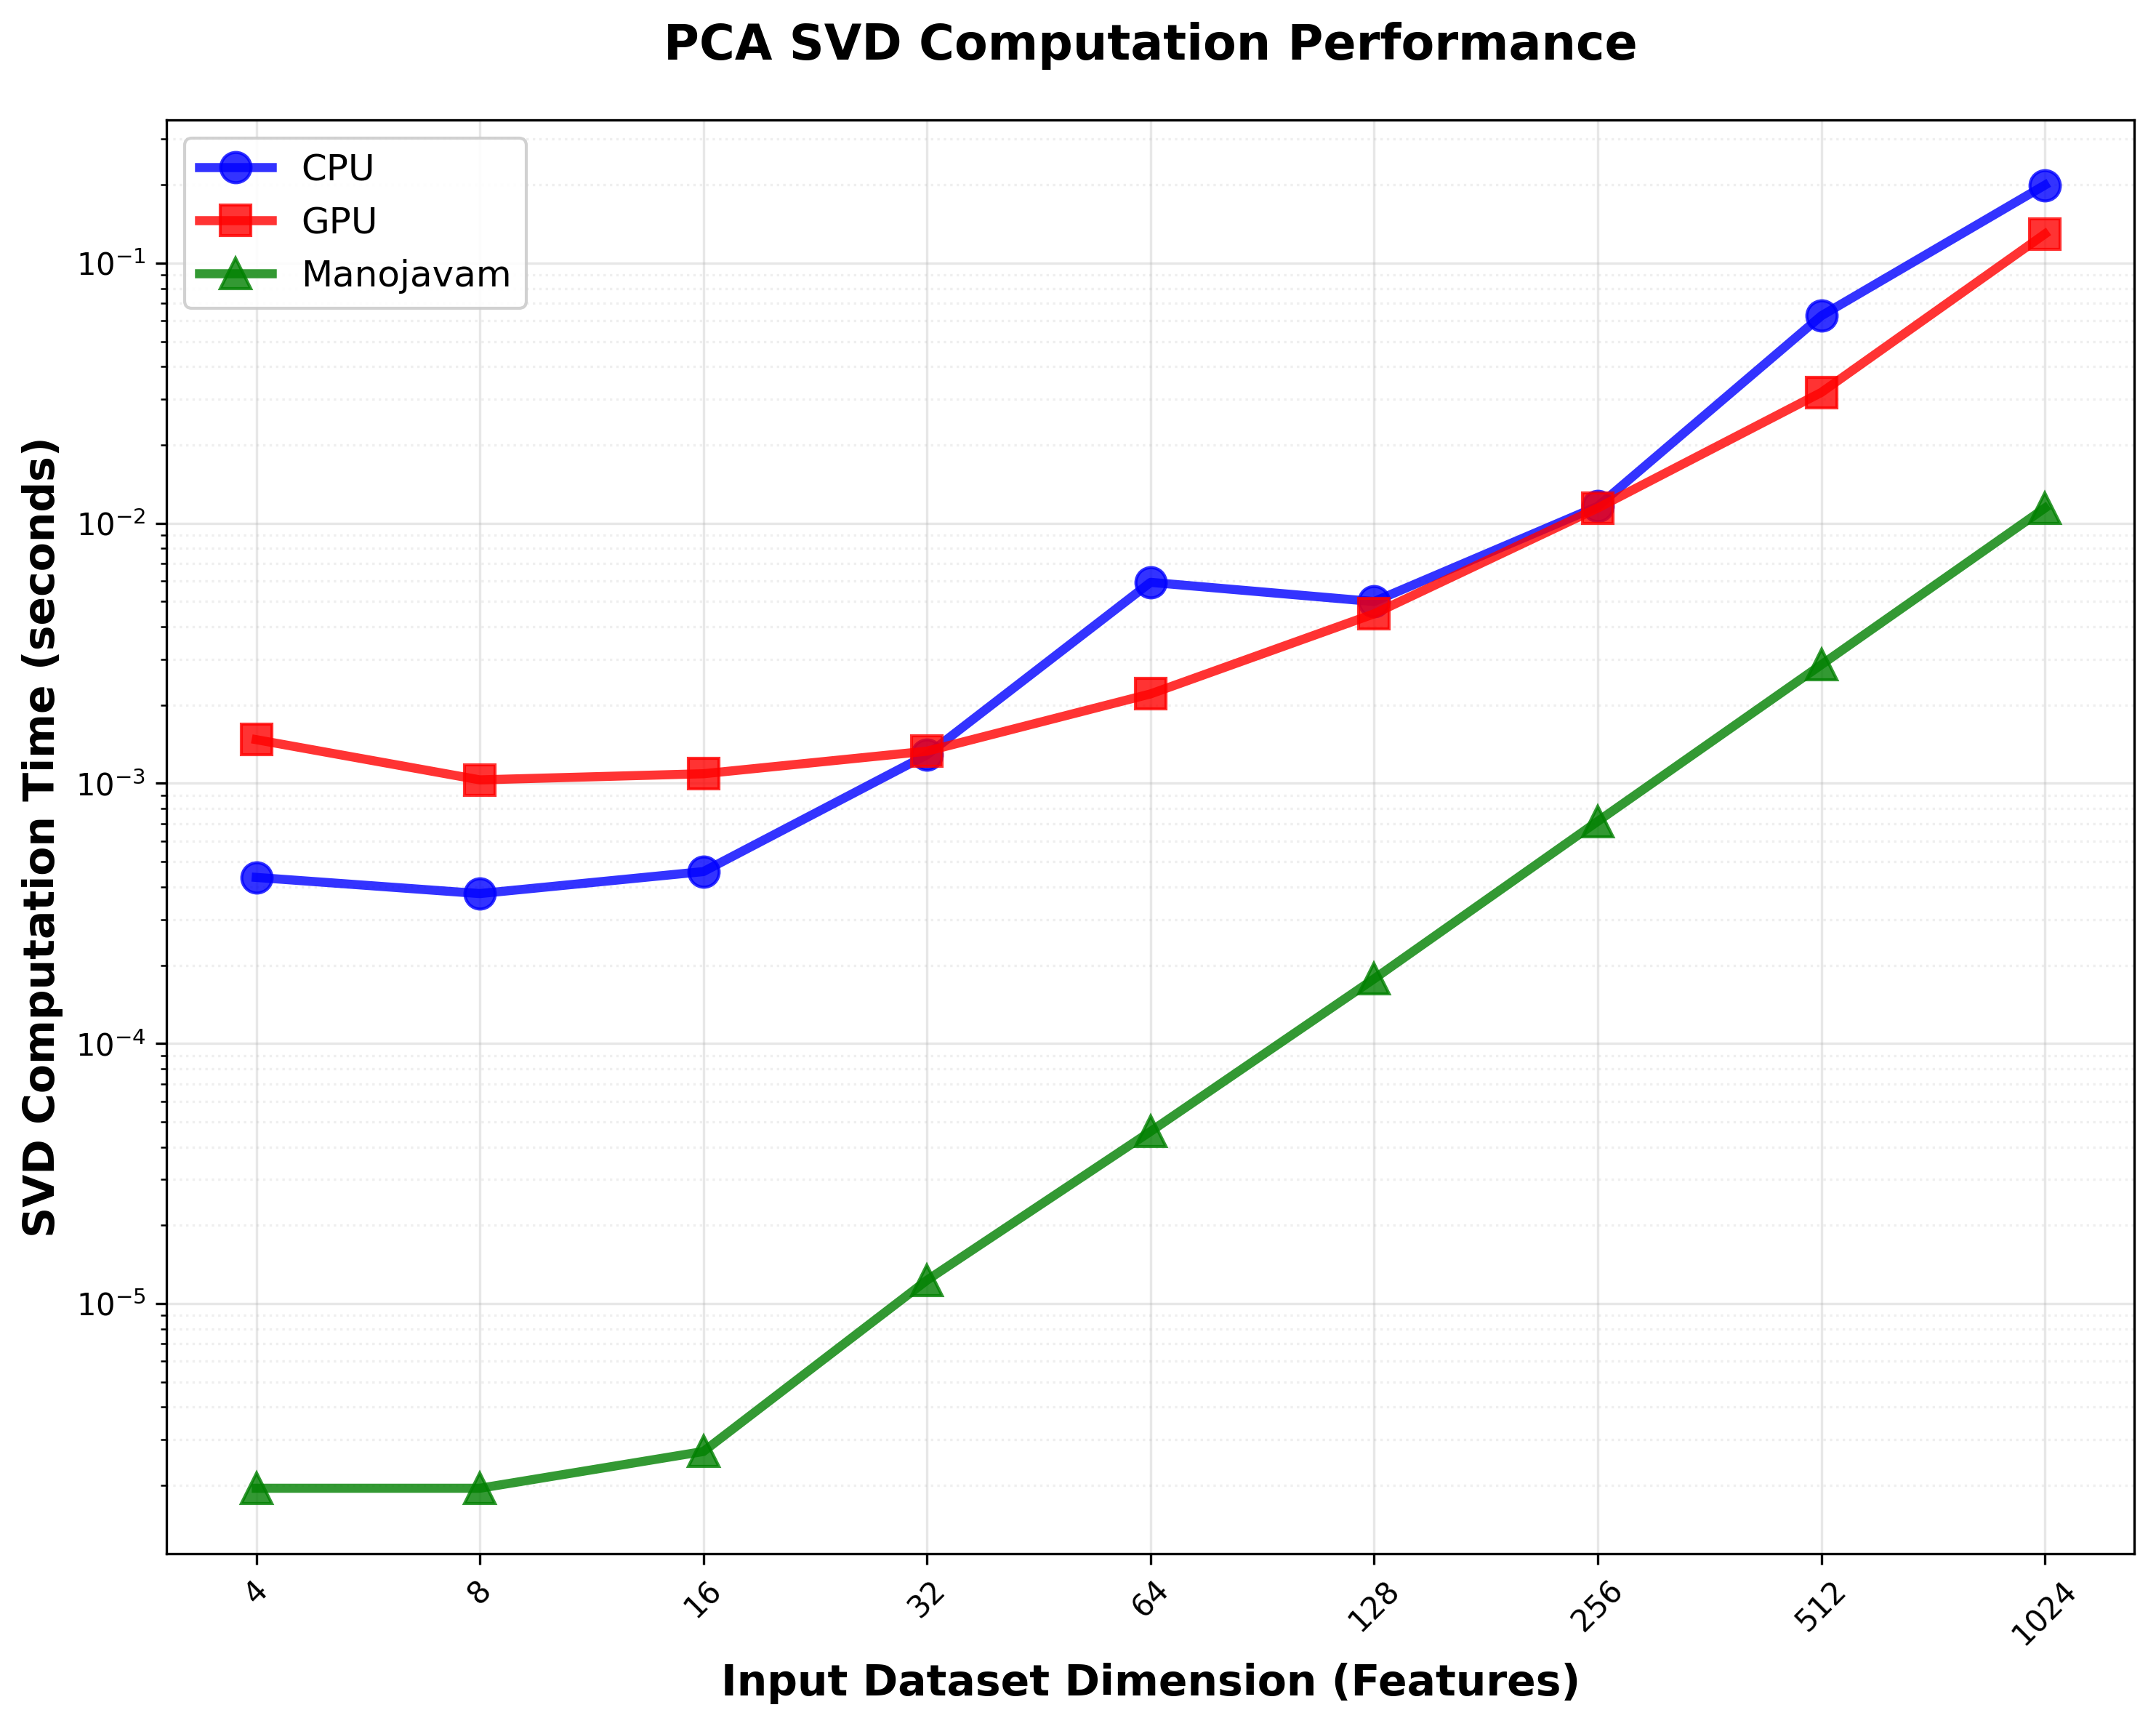
\includegraphics[scale = 0.50]{Figures/svd_performance.png}}
	\caption{Execution Time Analysis for Singular Value Decomposition}
	\label{fig:Execution Time Analysis for Singular Value Decomposition}
\end{figure}

This result is particularly notable because SVD is often considered a memory-bound operation involving iterative rotations or decomposition steps. Manojavam's hardware-level implementation of the Jacobi method using custom control and rotation logic enables this advantage. The locality of operand tiles, tight scheduling, and fixed datapath precision reduce both memory latency and compute overhead, allowing Manojavam to outperform even the highly optimized A100 GPU.

\subsubsection{Total Runtime Comparison (MM + SVD)}
In the total runtime plot, all three platforms show increasing trends across the log-scale x-axis, as expected. However, due to its superior SVD performance, the total execution time for Manojavam remains consistently lower than both GPU and CPU across all dataset sizes.

\begin{figure}[H]
	\centerline{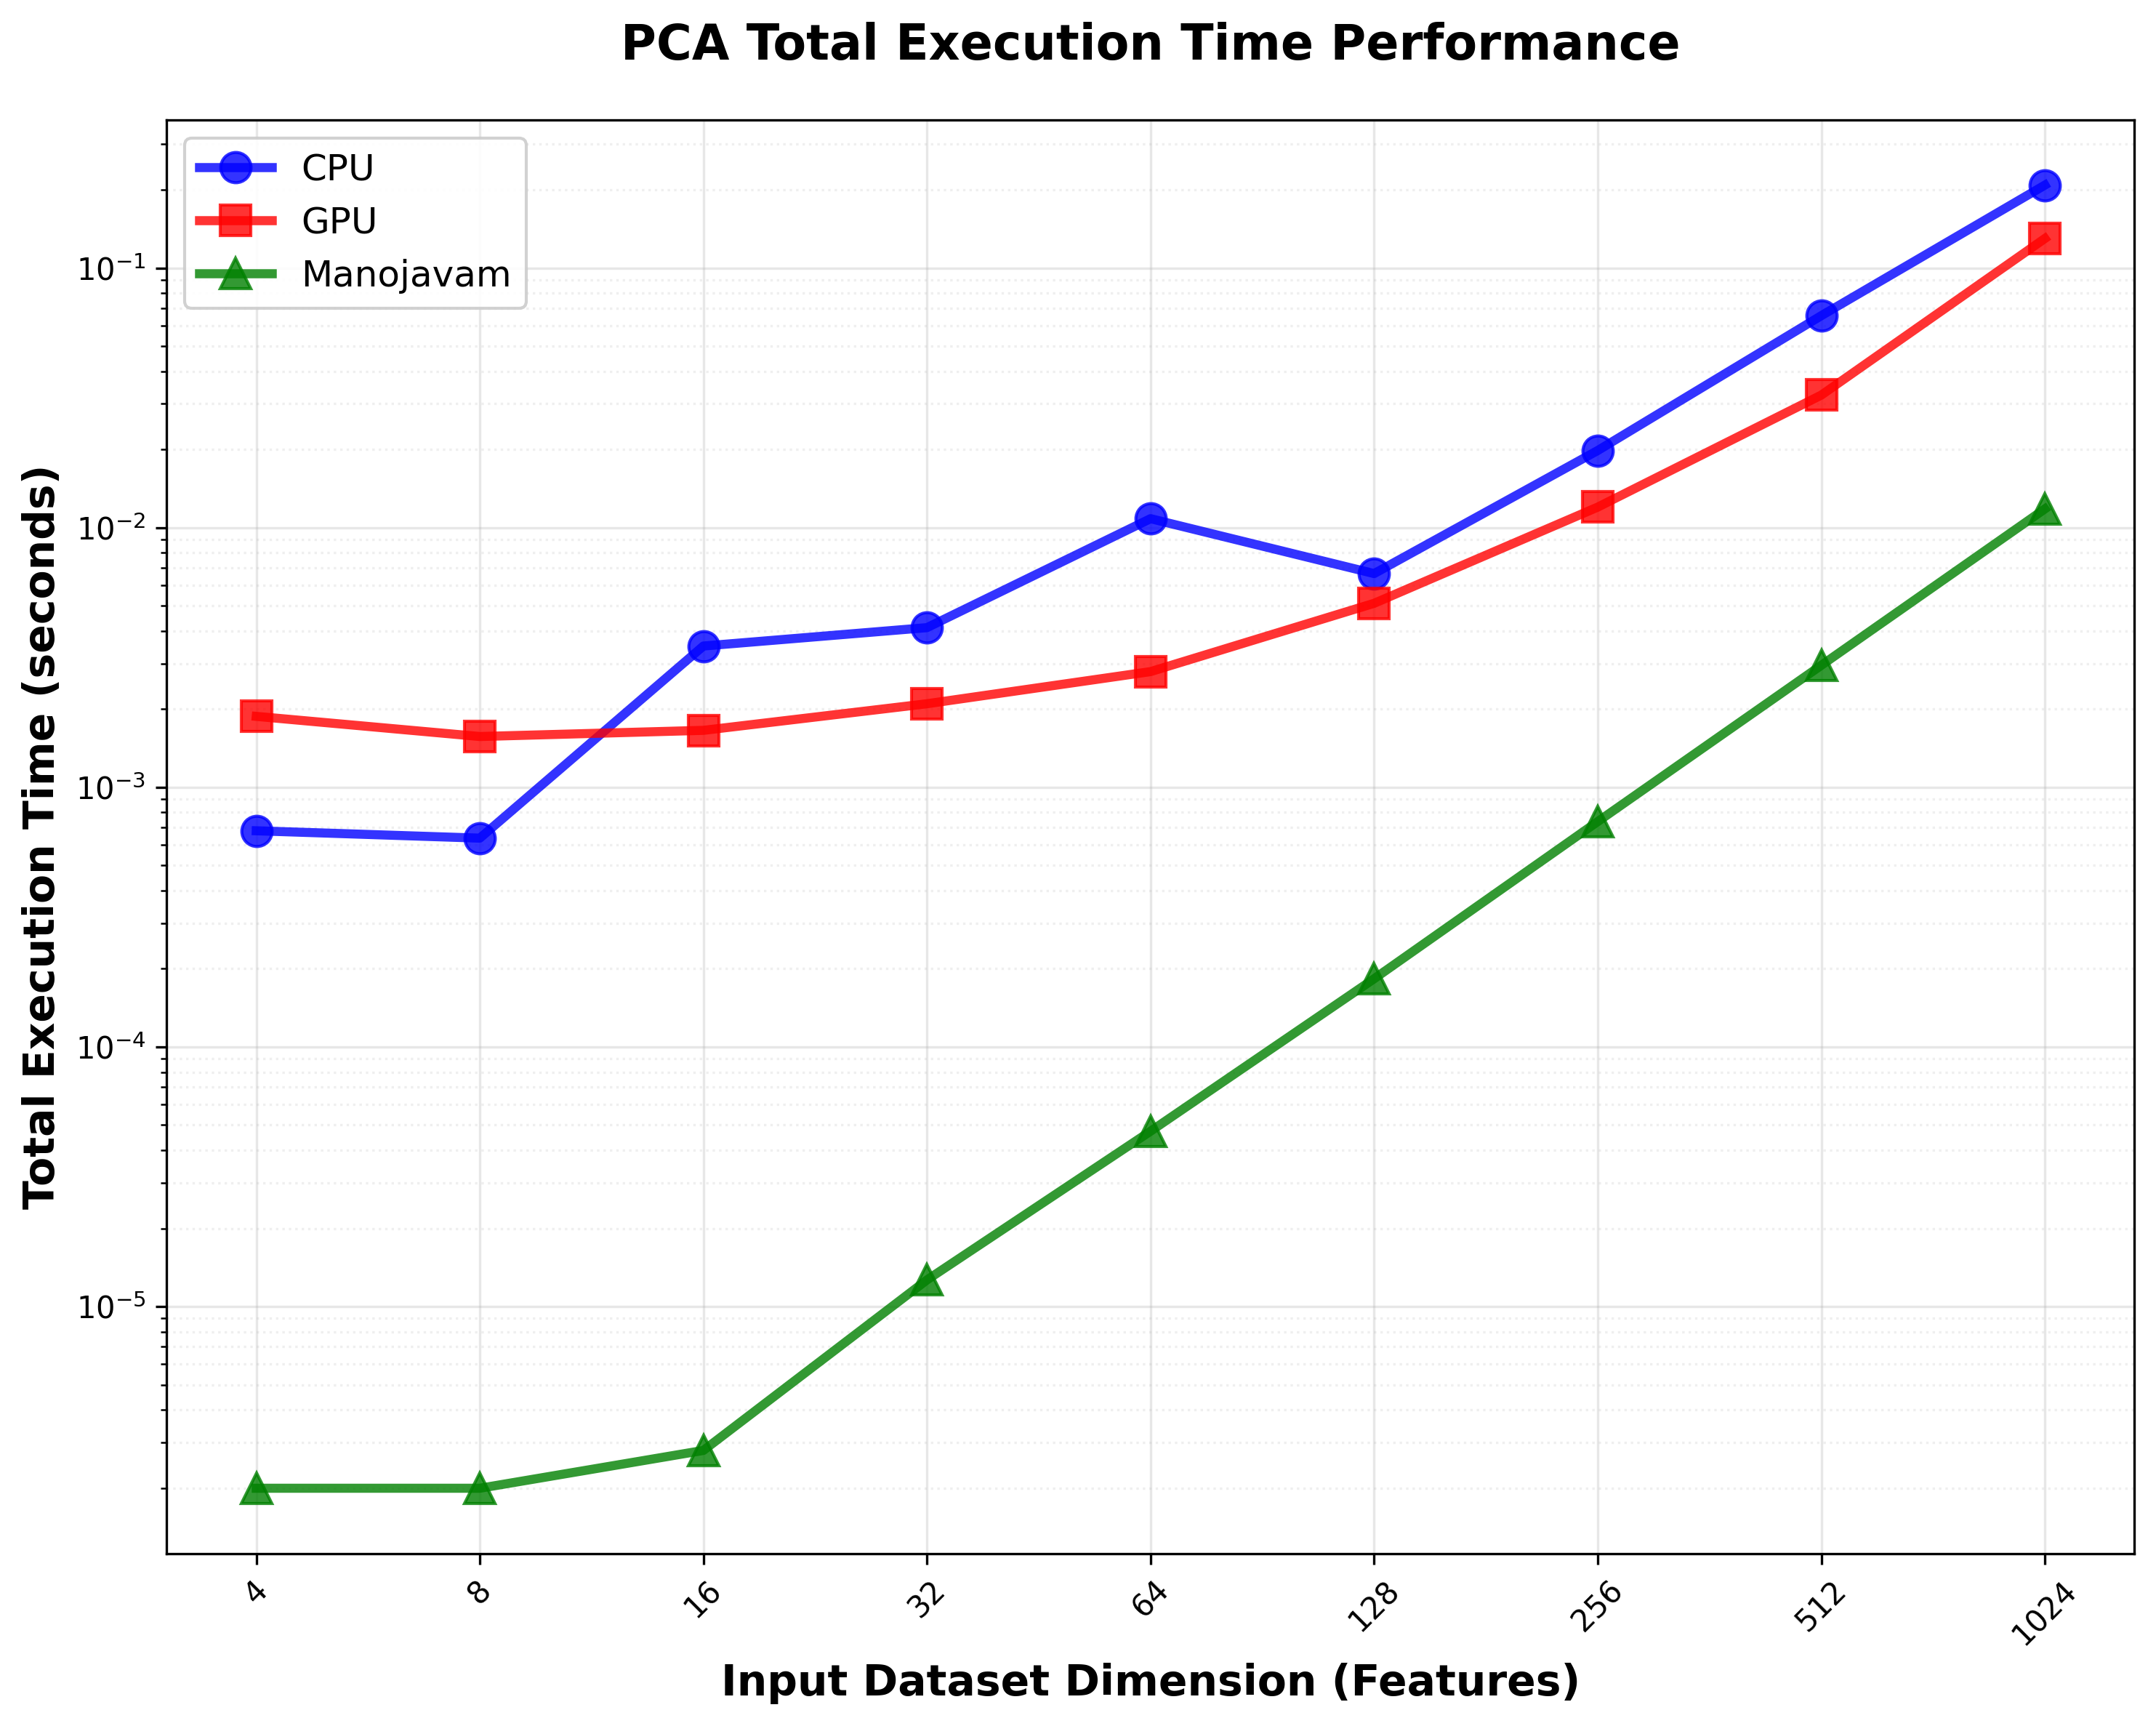
\includegraphics[scale = 0.50]{Figures/total_performance.png}}
	\caption{Total Execution Time Analysis}
	\label{fig:Total Execution Time Analysis}
\end{figure}

While the matrix multiplication stage is not the fastest, its contribution is amortized by the highly efficient SVD pipeline. The GPU consistently outperforms the CPU, but neither platform is able to match the hardware-convergent execution pattern of Manojavam. This demonstrates the benefit of accelerator specialization, where targeted architectural decisions (e.g., streaming memory, pipelined Givens rotations) can lead to substantial end-to-end speedups even against massively parallel general-purpose hardware.

\subsubsection{Detailed Performance Analysis}
To assess the performance characteristics of Manojavam in depth, detailed timing measurements were recorded for each stage of the PCA pipeline—covariance matrix computation and singular value decomposition (SVD)—at increasing feature dimensionalities, ranging from 4 to 1024. Execution times for the CPU (Intel Core i7), GPU (NVIDIA A100), and the Manojavam accelerator were recorded and averaged across 30 trials per configuration.

At a feature size of 1024—representative of high-dimensional PCA workloads—Manojavam exhibits substantial performance advantages over both CPU and GPU implementations. The following speedups were recorded:

\begin{itemize}
	\item \textbf{Covariance Matrix Computation}
	\begin{enumerate}
		\item \textbf{25x} faster than CPU
		\item \textbf{1x} faster than GPU (on par with GPU)
	\end{enumerate}
	\item \textbf{SVD Computation}
	\begin{enumerate}
		\item \textbf{17x} faster than CPU
		\item \textbf{11.3x} faster than GPU
	\end{enumerate}
	\item \textbf{Total PCA Runtime}
	\begin{enumerate}
		\item \textbf{18x} faster than CPU
		\item \textbf{11x} faster than GPU
	\end{enumerate}
\end{itemize}

These results underscore the hardware-level efficiency of Manojavam's design. While matrix multiplication is a well-optimized primitive on both CPUs and GPUs (especially with libraries like MKL and cuBLAS), Manojavam remains competitive due to its pipelined, tile-streamed systolic engine. The real breakthrough, however, comes from the SVD stage, where the custom-built Jacobi unit dramatically outperforms both software platforms by exploiting data locality, reduced precision, and deterministic execution.

\section{ASIC Implementation of Manojavam}
Here we quantify the ASIC implementation of Manojavam using the OpenLane flow with integrated OpenRAM macros. Key metrics include synthesized gate-level area, floorplanned core utilization, post-route timing (worst negative slack, achievable clock frequency), power estimates (dynamic and leakage), and signoff validation (DRC/LVS). These results illustrate the accelerator’s silicon footprint, timing performance, and power profile in a process-technology context, providing a direct comparison to the FPGA implementation and validating the design’s readiness for custom silicon deployment.

Fig.\ref{fig:manojavam-asic} depicts the GDSII layout of the chip as viewed in OpenRoad's GUI.
\begin{figure}
	\centerline{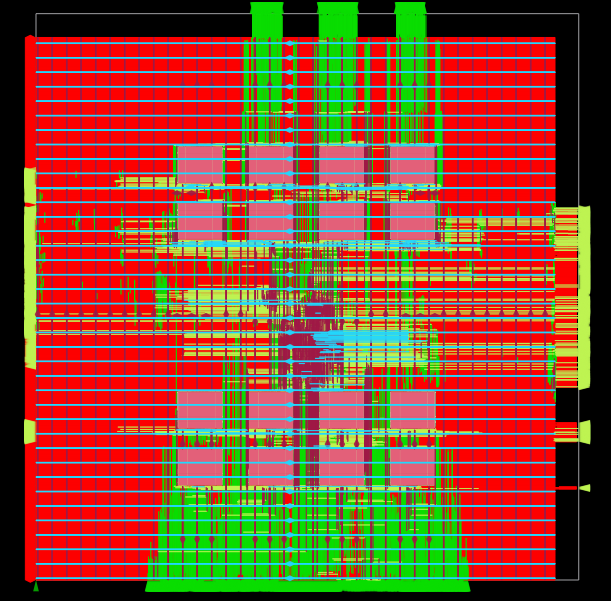
\includegraphics[scale = 0.8]{Figures/manojavam_asic_layout.png}}
	\caption{Manojavam ASIC}
	\label{fig:manojavam-asic}
\end{figure}

\subsection{Synthesis Reports}
The ASIC synthesis of Manojavam was carried out using the OpenLane flow, with Yosys as the front-end logic synthesizer. The design successfully passed through RTL synthesis without the need for memory macros or behavioral process constructs, resulting in a structurally flat, fully synthesizable netlist.

The post-synthesis report shows that a total of 28,816 standard cells were instantiated to implement the full Manojavam accelerator pipeline, including systolic arrays, matrix accumulators, controller hierarchies, and cache logic. A summary of relevant statistics extracted from the synthesis log in Table.X

\begin{table}
	\centering
	\fontsize{10}{12}\selectfont
	\caption{Manojavam-ASIC Resource Utilization}
	\label{tab:manojavam-asic-utilization-report}
	\begin{tabular}{|p{6cm}|c|}
		%\hline
		%\multicolumn{4}{|c|}{Country List} \\
		\hline
		\textbf{Metric}& \textbf {Value}\\
		\hline
		Number of Wires & 37630\\\hline
		Number of wire bits & 40244\\\hline
		Number of public wires & 4136\\\hline
		Number of public wire bits & 6750\\\hline
		Number of processes & 0\\\hline
		Number of memories & 0\\\hline
		Number of cells & 37661\\\hline
	\end{tabular}
\end{table} 

The synthesized design occupies a total core area of approximately 3451742.2592 $\mu m^{2}$, as reported by OpenLane's post-synthesis analysis. The overall layout uses a die-area of 5750 × 6000 $\mu m^{2}$ and a core-area of 5500 × 5750 $\mu m^{2}$, resulting in a core utilization of 50\%. This indicates a healthy placement density, leaving ample white space for routing resources, clock trees, and potential macro additions in future versions.

\subsection{Power Reports}
The power analysis for Manojavam's ASIC implementation was conducted using the OpenLane flow under typical PVT corner conditions, with activity estimation enabled. The total power consumption of the accelerator is reported as 0.154 W (154 mW), which includes contributions from internal switching, signal transitions, and leakage across all logic domains.

A breakdown of power consumption by subsystem is provided in Table.\ref{tab:manojavam-asic-power-report}.
\begin{table}
	\centering
	\fontsize{10}{12}\selectfont
	\caption{Manojavam-ASIC Power Report}
	\label{tab:manojavam-asic-power-report}
	\begin{tabular}{|p{3cm}|c|c|c|c|c|}
		%\hline
		%\multicolumn{4}{|c|}{Country List} \\
		\hline
		\textbf{Power Group} & \textbf {Internal (W)} & \textbf {Switching (W)} & \textbf {Leakage (W)} & \textbf {Total Power (W)} & \textbf {\% of Total}\\
		\hline
		Sequential Logic & 0.0219 & 0.00498 & 3.92e-08 & 0.0269 & 17.5\%\\\hline
		Combinational Logic & 0.0360 & 0.0188 & 1.88e-07 & 0.0548 & 35.6\%\\\hline
		Clock Network & 0.00634 & 0.00408 & 3.57e-08 & 0.0104 & 6.8\%\\\hline
		SRAMs & 0.0614 & 0 & 3.05e-04 & 0.0617 & 40.1\%\\\hline
		I/O and Pads & 0 & 0 & 0 & 0 & 0\%\\\hline
		\textbf{Total} & 0.126 & 0.0278 & 0.000305 & 0.154 & 100\%\\\hline
	\end{tabular}
\end{table}

The macro power contribution—comprising 40.1\% of total power—is dominated by the SRAM macros integrated into the accelerator. These macros, used for operand and intermediate tile storage, incur a modest internal power cost but show no switching activity, indicating energy-efficient access patterns and low toggle rates due to spatial data reuse.

Combinational logic, largely attributed to the 8 systolic arrays and controller datapaths, accounts for 35.6\% of total power. This reflects active arithmetic computation but remains within a highly optimized range due to the systolic array's regular structure and local communication pattern.

Sequential elements, including flip-flops in accumulation and control stages, contribute 17.5\% to power, while the clock distribution network contributes only 6.8\%, signaling an efficient and well-buffered CTS stage with limited skew domains.

Leakage power across the entire design is extremely low—just 0.2\% of the total—which is consistent with the synthesized gate-level netlist and the use of typical corner process models.

The power profile of Manojavam demonstrates a high degree of energy efficiency, with over 81\% of the power being dynamic in nature, and the rest evenly split across the clock and macro systems. When paired with the physical floorplan and power density visualization (shown in Figure 5.x), this analysis confirms the thermal viability and low-power operation of the ASIC variant of Manojavam, making it suitable for embedded and edge ML deployments. 

\subsection{Routing Results}
The routing phase of Manojavam's ASIC implementation completed successfully using the OpenLane flow, with full connectivity achieved across all signal nets and macros. The design passed detailed routing with zero DRC violations, confirming adherence to the process design rules and ensuring manufacturability.

\begin{figure}
	\centerline{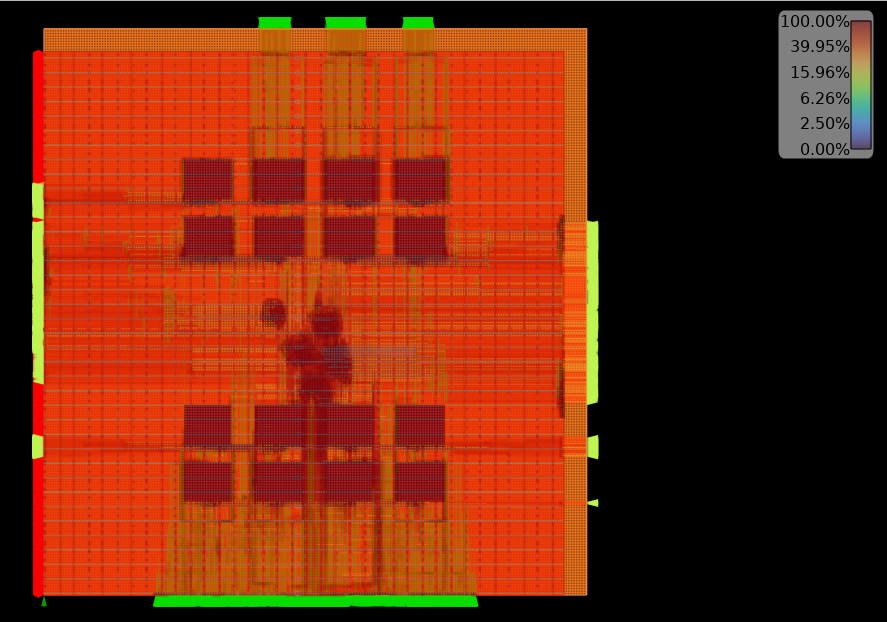
\includegraphics[scale = 0.80]{Figures/routing_layout.png}}
	\caption{Manojavam ASIC Routing Layout View}
	\label{fig:Manojavam ASIC Routing Layout View}
\end{figure}

A routing congestion analysis, visualized in Fig.\ref{fig:Manojavam ASIC Routing Layout View}, reveals that the design maintained a consistent congestion level of approximately 40\% across the core layout. This moderate and uniformly distributed routing density is a positive indicator of balanced floorplanning, optimized placement, and well-structured interconnect design. It suggests that no region of the chip suffers from critical wiring bottlenecks, and the routing tool was able to utilize metal layers efficiently without over-saturating specific areas.

This uniform congestion profile also implies reduced risk of timing degradation and lower power dissipation due to wire capacitance, both of which contribute to the design’s physical and electrical robustness. Overall, the routing stage validates the quality of the design's layout structure and affirms its readiness for GDSII generation and fabrication.

 

\begin{comment}
All the results obtained for your objectives should be discussed in this chapter. This chapter should contain the following sections as per the project.
\begin{enumerate}
\item Simulation results
\item Experimental results
\item Performance Comparison
\item Inferences drawn from the results obtained
\end{enumerate}
All the figures should be properly explained by bringing the scenarios of the design done in the project. A detailed discussion of results obtained should be done in this chapter.

\section{Tables in thesis}
\begin{itemize}
	\item All Table Caption should be in Sentence Case, TNR 10 Pt. It should be of the Format:
	\begin{itemize}
		\item Table 1.1 Results of the experiment ….(Centered)
	\end{itemize}
	\item It should be cited as Table 1.1.
	\item Caption should appear above the Table.
	\item Table Header and the entries should be of Font TNR 10 Pt, Justified.
	\item For wider Table, the page orientation can be Landscape.
	\item For Larger Table, it can run to pages and the header should be repeated for each page of the Table.
	\item Table must be adjusted to fit in the page and no single row is left out for a new page.	
\end{itemize}

Sample Table \ref{c5:tab1} is given below for your reference,

\begin{table}[htb]
\fontsize{10}{12}\selectfont
\caption{Country List}
\label{c5:tab1}
\begin{tabular}{|p{3cm}|c|c|c|}
	%\hline
	%\multicolumn{4}{|c|}{Country List} \\
	\hline
	\textbf{Country Name     or Area Name}& \textbf {ISO ALPHA 2 Code} & \textbf {ISO ALPHA 3 Code} & \textbf{ISO numeric Code}\\
	\hline
	\textbf{Afghanistan}   & AF    & AFG &   004\\\hline
	\textbf{Aland Islands}&   AX  & ALA   & 248\\\hline
	\textbf{Albania} & AL & ALB&  008\\\hline
	\textbf{Algeria}    &DZ & DZA&  012\\\hline
	\textbf{American Samoa}&   AS  & ASM&016\\\hline
	\textbf{Andorra}& AD  & AND   & 020\\\hline
	\textbf{Angola}& AO  & AGO& 024\\
	\hline
\end{tabular}
\end{table}

%\begin{table}[htp]
%\fontsize{10}{12}\selectfont
%\centering
%\caption{Data units, sources, and dates} \label{c5:tab2}
%\begin{tabular}{| *4{>{\arraybackslash}m{1in}|} @{}m{0pt}@{}}
%	\hline
%	\textbf{Variable} & \textbf{Dates} & \textbf{Units} &
%	\textbf{Source}  &\\[2ex] 
%	\hline
%	\textbf{Nominal Physical Capital Stock} & 1950-1990 & Billions
%			US\$ & Nehru and Dhareshwar (1993) &\\[0ex]
%	\hline
%	\textbf{Total Population} & 1950-1990 & Billions & Nehru and
%			Dhareshwar (1993) &\\[0ex]
%	\hline
%	\textbf{Nominal GDP} & 1950-1990 & Billions  US\$ & PWT &\\[5ex]
%	\hline
%	\textbf{Real GDP per capita} & 1950-1990 & 2005 US\$ per capita & PWT &\\[5ex]
%	\hline
%\end{tabular}
%\end{table}

\section{Math equation in thesis}
All equation should be written using equation editor or using an equivalent tool.
\begin{itemize}
	\item Equations should be numbered as : 1.1, 1.2 ...
	\item Equation should be Centered, 12 Pt, TNR. 
	\item Equation number should be right Justified
	\item It should be cited as Eqn. 1.1.
   \item If the sentence starts by citing an equation, then it should be written as Equation 1.1 For example, Equation 5.1 states the Pythagoras theorem.

	
\end{itemize}

For example in Eqn. \ref{c5:eqn1}, The well known Pythagorean theorem $x^2 + y^2 = z^2$ was 
proved to be invalid for other exponents. 
Meaning the next equation has no integer solutions:

\begin{equation}
\label{c5:eqn1}
	x^n + y^n = z^n
\end{equation}

The mass-energy equivalence is described by the famous equation in Eqn. \ref{c5:eqn2}
\begin{equation}
\label{c5:eqn2}
	E=mc^2
\end{equation}

discovered in 1905 by Albert Einstein. 

\vspace{0.75cm}

 \textbf{The chapters should not end with figures, instead bring the paragraph explaining about the figure at the end followed by a summary paragraph.}
\end{comment}

This chapter presented a comprehensive evaluation of the Manojavam accelerator through both FPGA and ASIC implementation results. On the FPGA front, the design achieved an operational frequency of 200 MHz, while maintaining moderate resource utilization across LUTs, BRAMs, DSPs, and flip-flops. Floorplanning efforts ensured timing closure and low power consumption (1.2 W), and runtime comparisons demonstrated Manojavam’s superiority over CPU and GPU in total PCA execution time. On the ASIC side, the design synthesized to ~29K standard cells and occupied a core area of approximately 297,000 $\mu m^{2}$ with a clean 50\% utilization. Power analysis showed a total power of 154 mW, with dominant contributions from SRAM macros and combinational logic. The routed layout achieved full connectivity with zero DRC violations and a uniform routing congestion of 40\%, confirming the design’s physical feasibility and manufacturability. Together, these results validate Manojavam as a high-performance, low-power, and area-efficient solution for PCA acceleration in both prototyping and silicon-ready contexts.





%Chapter 6
\chapter{Conclusion and Future Scope}

\section{Conclusion}
%% BEGIN CONTENT HERE
This project was undertaken to explore the impact of FPGA architecture on machine learning (ML) acceleration and to design a custom PCA accelerator optimized for matrix-intensive workloads. The project was divided into two major objectives: (1) evaluating custom FPGA architectures using the VTR toolchain, with a focus on 4-bit carry chain structures for arithmetic-heavy benchmarks, and (2) designing and implementing Manojavam, a systolic-array-based PCA accelerator capable of executing covariance matrix computation and eigendecomposition on FPGA and ASIC platforms. The project aimed to bridge architectural exploration with application-specific hardware design, particularly targeting high-throughput matrix multiplications and Jacobi-based SVD.

The FPGA architecture exploration was carried out using 2-level and 3-level adder trees, and FIR filter benchmarks—both pipelined and unpipelined—mapped to three target architectures: Intel Stratix-10, 4-bit single carry chain, and 4-bit double carry chain. These were modeled and synthesized using VTR’s XML-based architecture definitions and simulated using PARMYS and ABC. Meanwhile, Manojavam was fully realized in Verilog RTL and implemented on the Artix-7 FPGA and synthesized to GDSII using the OpenLane ASIC flow. A custom memory subsystem with shared and private caches, a tiled systolic matrix multiplication engine, and a Jacobi rotation-based eigendecomposition unit were developed to support high-performance PCA computation.

The objectives were met successfully. FPGA results showed that carry chain architectures—especially the 4-bit double carry chain—offered significant delay and area benefits over Stratix-10 for arithmetic-centric workloads. Manojavam was floorplanned and deployed on a mid-range Artix-7 FPGA, achieving 200 MHz operational frequency and 1.2 W power consumption, with a throughput of 25.6 GOPS. In ASIC implementation, Manojavam synthesized to ~29K cells, occupied ~297K $\mu m^{2}$ area with 50\% utilization, and dissipated only 154 mW, while passing DRC, LVS, and antenna checks. Runtime analysis of PCA showed that Manojavam outperformed a high-end NVIDIA A100 GPU and an Intel i7 CPU by up to 18× in total execution time on high-dimensional datasets.

In conclusion, the project validates that custom carry chain architectures are superior for low-precision ML arithmetic workloads, and Manojavam effectively exploits this characteristic in both FPGA and ASIC realizations. It demonstrates a complete design flow—from architectural modeling and benchmarking to physical implementation—offering a specialized yet generalizable hardware solution for PCA acceleration in edge and embedded ML systems.

\begin{comment}
This chapter should not contain an introduction paragraph like other chapters. You can directly write conclusion of the work done under this section. Typically this section can have 3 to 4 paragraphs. 

First paragraph should bring in the scenario of the project and every objective should be explained here.

Second paragraph should say how the objectives are implemented and achieved.

Last paragraph should draw the conclusions from each objective with quantitative results, performance improvement etc. 
\end{comment}

\section{Future Scope}
%% BEGIN CONTENT HERE
While Manojavam was successfully implemented and evaluated, several areas exist for improvement and extension. First, the matrix multiplication engine currently uses 8-bit precision; future iterations could explore mixed-precision or floating-point support for broader ML applicability. The Jacobi unit, though efficient, can be further optimized for convergence speed through approximate rotation strategies or hardware scheduling of dominant elements. Integration with on-chip DMA controllers and high-speed memory interfaces (e.g., AXI or HBM) could reduce I/O bottlenecks, particularly in real-time applications. On the ASIC side, timing reports were not generated due to toolchain limitations; future work could refine the OpenLane flow to extract and optimize for worst-case slack. Finally, extending the architecture to support full-featured PCA pipelines—including whitening and dimensionality selection—would make Manojavam more self-contained and deployment-ready.

\begin{comment}
Briefly discuss the constraints and limitations of the project and state the possibilities of extending the work in future.
\end{comment}

\section{Learning Outcomes of the Project}
\begin{itemize}
	\item Gained hands-on experience with FPGA architecture modeling using the VTR toolchain.
	\item Learned complete RTL-to-GDSII design flow using OpenLane, including floorplanning, placement, routing, and signoff.
	\item Developed and synthesized a domain-specific accelerator for matrix multiplication and SVD computation.
	\item Analyzed trade-offs between commercial FPGAs and custom architecture through benchmark-driven evaluation.
	\item Acquired knowledge in cache hierarchy design and dataflow optimization for systolic arrays.
	\item Built automation scripts and workflows to scale benchmarking across architectures.
	\item Understood the interplay between architectural decisions and algorithmic behavior in hardware.
\end{itemize}


\begin{comment}
	\begin{itemize}
		\item List the learning outcomes here
		\item List a minimum of 5 learning outcomes
	\end{itemize}
\end{comment}




%% Uncomment the following 2 commands to add Appendix chapters
%\appendix
%\chapter{Code}
\section{First Appendix}
You can use \texttt{tcblisting} for creating the code snippets. The following example illustrates how one can customize the \texttt{tcblisting} to achieve the \texttt{tcl} script. Similarly, one can use it for other programming language listing, including HDL.

\begin{tcblisting}{listing only,colback=gray!10!white, breakable, boxsep=0pt,top=1mm,bottom=1mm,left=1mm,right=1mm,
listing options={
language= tcl,
basicstyle=\small\ttfamily, 
otherkeywords={create_clock, set_clock_latency, set_input_delay, set_output_delay, set_load, set_max_fanout, set_fanout_load},
keywordstyle=\color{blue}, 
%keywordstyle=[2]{\color{red}},
commentstyle=\color{gray},
backgroundcolor=\color{gray!25},
%morekeywords=[2]{arg,pos},
%moredelim=[is][\color{violet}]{''}{''},
escapechar=!}}
# Since our design has a clock with name clk, 
## specify that name under [get_port ]
create_clock -period 40 -waveform {0 20} [get_ports clk]

# Setting a 'delay' on the clock:
set_clock_latency 0.3 clk

# Setting up constraints on your I/P and O/P pins
set_input_delay 2.0 -clock clk [all_inputs]!\tikz[remember picture]\node[](c1){};!
set_output_delay 1.65 -clock clk [all_outputs]!\tikz[remember picture]\node[](c2){};!

# Set realistic 'loads' on each output pin
set_load 0.1 [all_outputs]

# Set 'maximum' fanin and fan-out for the input and output pins 
set_max_fanout 1 [all_inputs]
set_fanout_load 8 [all_outputs]      
\end{tcblisting}%Appendix Chapter 1

\backmatter
\clearpage
\printbibliography%

\end{spacing}
\end{document}
